\documentclass[11pt]{amsart}
\usepackage[T1]{fontenc}
\usepackage{lmodern,microtype,amsmath,amssymb,amsthm,mathtools,mathrsfs}
\usepackage[margin=1in]{geometry}
\usepackage{booktabs,longtable,array,xcolor,tikz}
\usepackage{float}
\usetikzlibrary{arrows.meta,decorations.pathreplacing}
\definecolor{cellblue}{RGB}{31,75,115}
\usepackage[hidelinks]{hyperref}
\hypersetup{pdftitle={Nonunique selection for two-dimensional Euler with finite-Lp vorticity},pdfauthor={Tao Tao and Haiqi Zhang}}
\newtheorem{theorem}{Theorem}[section]
\newtheorem{lemma}[theorem]{Lemma}
\newtheorem{proposition}[theorem]{Proposition}
\newtheorem{corollary}[theorem]{Corollary}
\newtheorem{problem}[theorem]{Problem}
\theoremstyle{remark}
\newtheorem{remark}[theorem]{Remark}
\numberwithin{equation}{section}
\newcommand{\norm}[1]{\left\lVert#1\right\rVert}
\newcommand{\R}{\mathbb R}
\newcommand{\C}{\mathbb C}
\newcommand{\T}{\mathbb T}
\newcommand{\dd}{\,\mathrm d}
\setlength{\emergencystretch}{2em}
\title[Nonunique selection for two-dimensional Euler]{Nonunique selection for two-dimensional Euler\\
with vorticity in a prescribed finite $L^p$ space}
\author[T.~Tao]{Tao Tao}
\address{School of Mathematics, Shandong University,
Jinan 250100, P.~R.~China}
\email{taotao@sdu.edu.cn}
\author[H.~Zhang]{Haiqi Zhang}
\address{School of Mathematics, Shandong University,
Jinan 250100, P.~R.~China}
\email{ZHQAQ2024@outlook.com}
\date{}
\begin{document}

\begin{abstract}
We study nonuniqueness for the unforced incompressible Euler equations
on the square two-dimensional torus with vorticity uniformly bounded in
a prescribed finite $L^p$ space. The construction starts from a stationary
sum of concentric, zero-circulation, two-interface vortices. A nonstationary
ancient orbit of one vortex provides a fourth angular mode; a bilateral
moment transform selects a strength ratio for which that mode seeds the
next larger vortex. We give the contour-space spectral reduction,
continuous passage through a geometric exit section, separated-field
estimates, and a finite-stage induction with constants independent of
the number of scales. Strong compactness preserves a fixed departure
from the stationary datum. For each $1<p<\infty$, the resulting datum
admits an uncountable family of distinct weak solutions with
$L^\infty_tL^p_x$ vorticity. An auxiliary exponent greater than two gives
Lipschitz continuity in time with values in $L^2$ and conservation of
kinetic energy. All parameters, including the datum, may depend on $p$.
\end{abstract}

\maketitle

\tableofcontents

\section{Introduction}\label{sec:introduction}
\subsection{The question and its mathematical context}
The two-dimensional incompressible Euler equations on
$\T^2\coloneqq(\R/2\pi\mathbb Z)^2$ are
\begin{equation}\label{intro:euler}
 \partial_tu+\operatorname{div}(u\otimes u)+\nabla\pi=0,
 \qquad \operatorname{div}u=0,
 \qquad \omega\coloneqq\partial_1u_2-\partial_2u_1.
\end{equation}
Here $u$ is the velocity, $\pi$ the pressure, and $\omega$ the scalar
vorticity; the torus carries ordinary Lebesgue measure, of total mass
$4\pi^2$. For smooth solutions,
\begin{equation}\label{intro:transport}
 \partial_t\omega+u\cdot\nabla\omega=0,
 \qquad u=K_{\T^2}*\omega
\end{equation}
when the velocity has mean zero. The normalization of $K_{\T^2}$ is
specified in Section~\ref{sec:preliminaries}.

Yudovich's theorem \cite{Yudovich1963} gives global existence and
uniqueness for bounded vorticity. The central mechanism is a
logarithmic modulus of continuity of velocity whose reciprocal satisfies
the Osgood divergence criterion. On the torus, every mean-zero initial
vorticity in $L^p$, $1<p<\infty$, admits a global weak solution with
vorticity bounded in $L^\infty_tL^p_x$ \cite{DiPernaMajda1987}.
The corresponding fixed-exponent estimates do not supply that
uniqueness argument.
The distinction concerns a bound throughout positive times, rather
than regularity of the initial datum alone.

For the forced equation, Vishik's theorem and subsequent proofs give
nonuniqueness with simultaneous $L^1$ and $L^q$ vorticity bounds for
every prescribed $q>2$ \cite{VishikI,VishikII,VishikBook,CFMS}.
Interpolation gives the corresponding bound for any prescribed
$1<p<\infty$. These are results for one common prescribed force.
For the unforced equation, Bru\`e and Colombo \cite{BrueColombo2023}
constructed solutions with weak-$L^1$ vorticity, and Bru\`e, Colombo,
and Kumar \cite{BCK2024} obtained $L^\infty_tL^p_x$ vorticity for
some $p>1$. Mengual's theorem \cite{Mengual2024} imposes finite-$L^p$
vorticity on the initial datum; it does not impose the same bound at
positive times. None of these statements is used here as a theorem
giving the unforced, arbitrary-prescribed-exponent conclusion below.

We use the following velocity formulation. A divergence-free
$u\in C([0,T];L^2(\T^2;\R^2))$ with $u(0)=u_0$ is a weak solution if
\begin{equation}\label{intro:weak}
 \int_0^T\!\!\int_{\T^2}
 \bigl[u\cdot\partial_t\varphi+
       (u\otimes u):\nabla\varphi\bigr]\,dx\,dt
 +\int_{\T^2}u_0\cdot\varphi(0,x)\,dx=0
\end{equation}
for every divergence-free
$\varphi\in C_c^\infty([0,T)\times\T^2;\R^2)$.
The matrix contraction is $A:B\coloneqq\sum_{i,j}A_{ij}B_{ij}$.

\subsection{Main results and the meaning of nonunique selection}
\begin{theorem}[Nonunique selection at a prescribed finite exponent]
\label{main}
For every $T>0$ and $p\in(1,\infty)$, there exist
\[
 u_0\in L^2(\T^2;\R^2)\cap W^{1,p}(\T^2;\R^2),\qquad
 u^{(1)},u^{(2)}\in C([0,T];L^2(\T^2;\R^2))
\]
such that
\[
 \operatorname{div}u_0=0,\qquad \int_{\T^2}u_0\,dx=0,\qquad
 u^{(1)}(0)=u^{(2)}(0)=u_0,
\]
each $u^{(i)}$ satisfies \eqref{intro:weak} and
$\operatorname{div}u^{(i)}=0$ in distributions, and
\[
 \max_{i\in\{1,2\}}
 \|\operatorname{curl}u^{(i)}\|_{L^\infty(0,T;L^p(\T^2))}<\infty,
 \qquad
 \int_0^T\|u^{(1)}(t)-u^{(2)}(t)\|_{L^2(\T^2)}^2\,dt>0.
\]
\end{theorem}

The two selections are a stationary solution and a nonstationary limit
of finite patch solutions whose data approach the same stationary
datum. Every finite approximation has bounded vorticity and its own
unique Yudovich evolution. Its $L^\infty$ vorticity bound is not uniform
in the number of scales. The limit is controlled in one fixed finite
exponent, so Yudovich uniqueness is not being invoked for it.

\begin{corollary}
\label{intro:refinement}
For every $T>0$ and $p\in(1,\infty)$, there exist
$q>\max\{p,2\}$, a datum $u_0$ as in Theorem~\ref{main}, an
uncountable set $I$, and weak Euler solutions
$(u^\theta)_{\theta\in I}$ on $[0,T]\times\T^2$ such that
\[
 u^\theta(0)=u_0\quad(\theta\in I),\qquad
 \sup_{\theta\in I}
 \|\operatorname{curl}u^\theta\|_{L^\infty(0,T;L^q(\T^2))}<\infty,
\]
\[
 u^\theta\in W^{1,\infty}(0,T;L^2(\T^2;\R^2)),\qquad
 \frac12\|u^\theta(t)\|_2^2=\frac12\|u_0\|_2^2
 \quad(\theta\in I,\ 0\le t\le T),
\]
and
\[
 \theta\ne\theta'\ \Longrightarrow\
 \int_0^T\|u^\theta(t)-u^{\theta'}(t)\|_2^2\,dt>0.
\]
\end{corollary}

In fact the proof fixes an auxiliary exponent
$q>\max\{p,2\}$ and obtains a uniform $L^q$ vorticity bound.
It does not produce one datum simultaneously for all finite exponents.
Energy conservation is a consequence of this auxiliary regularity;
the nonuniqueness mechanism is the selection of an evolution from a
stationary datum, rather than a choice of energy profile.

\subsection{The construction and its principal ideas}
The elementary cell and its scale parameters are
\begin{equation}\label{intro:definitions}
 a\coloneqq\sqrt{3/5},\qquad
 W\coloneqq\tfrac52\mathbf1_{B_a}-\tfrac32\mathbf1_{B_1},\qquad
 A_j\coloneqq A_0b^{-j},\qquad r_j\coloneqq R\rho^j .
\end{equation}
Here $B_r\coloneqq\{x\in\R^2:|x|<r\}$,
$0<b<1/4$, and $\rho>0$ is chosen much smaller than $b$.
The cell has value $1$ on $B_a$, value $-3/2$ on $B_1\setminus B_a$,
and zero elsewhere. Its circulation vanishes because
$(5/2)a^2-3/2=0$. Its velocity is tangential and vanishes outside
$B_1$; its exact profile is displayed in Figure~\ref{fig:cell}.

\begin{figure}[H]
\centering
\begin{tikzpicture}[x=3.1cm,y=1.15cm,>=Latex,font=\small]
 \draw[->] (-.08,0)--(1.5,0) node[right] {$r$};
 \draw[->] (0,-1.75)--(0,1.5) node[above] {$W(r)$};
 \draw[very thick,cellblue] (0,1)--(.77459667,1);
 \draw[very thick,cellblue] (.77459667,-1.5)--(1,-1.5);
 \draw[very thick,cellblue] (1,0)--(1.38,0);
 \draw[densely dashed,gray] (.77459667,-1.55)--(.77459667,1.06);
 \draw[densely dashed,gray] (1,-1.55)--(1,.15);
 \node[below] at (.77459667,0) {$a$};
 \node[above right] at (1,0) {$1$};
 \node[left] at (0,1) {$1$};
 \node[left] at (0,-1.5) {$-3/2$};
 \begin{scope}[xshift=6.0cm,yshift=-.8cm,y=3cm]
  \draw[->] (-.05,0)--(1.45,0) node[right] {$r$};
  \draw[->] (0,-.06)--(0,.64) node[above] {$v_\theta(r)$};
  \draw[very thick,cellblue] (0,0)--(.77459667,.38729833);
  \draw[very thick,cellblue,domain=.77459667:1,samples=50]
       plot (\x,{.75*(1/\x-\x)});
  \draw[very thick,cellblue] (1,0)--(1.34,0);
  \draw[densely dashed,gray] (.77459667,0)--(.77459667,.38729833);
  \node[below] at (.77459667,0) {$a$};
  \node[below] at (1,0) {$1$};
 \end{scope}
\end{tikzpicture}
\caption{Exact radial profiles of the isolated stationary cell:
$v_\theta(r)=r/2$ for $0\le r\le a$,
$v_\theta(r)=\tfrac34(r^{-1}-r)$ for $a\le r\le1$,
and $v_\theta(r)=0$ for $r\ge1$. The indicator coefficients are
$(g_1,g_2)=(5/2,-3/2)$. These are exact closed-form profiles.}
\label{fig:cell}
\end{figure}

The circular cell has an expanding fourth angular mode with rate
\[
 \sigma\coloneqq\frac{9\sqrt{15}}{100},\qquad
 \lambda_*\coloneqq\sigma-\frac34i.
\]
The finite-dimensional mode computation is related to
\cite[Section~3]{CFMS}; here the full contour-space spectral splitting
is established before applying the invariant-manifold theorem of
\cite{CFL2003}. It gives an ancient patch orbit $\Omega_*(s)$ tending
to $W$ as $s\to-\infty$. A geometric section defined by the
inner-domain fourth moment fixes its time origin.

The physical quantity that communicates with a larger vortex is
\begin{equation}\label{intro:moment-transform}
 N(s)\coloneqq\int_{\R^2}(x_1-ix_2)^4\Omega_*(s,x)\,dx,
 \qquad F(z)\coloneqq\int_\R e^{-zs}N(s)\,ds,
 \quad 0<\Re z<\sigma.
\end{equation}
The ancient tail is exponentially small and nonzero to leading order;
the positive-time moment grows at most polynomially. These facts make
$F$ holomorphic and nontrivial. A strength ratio $b$ outside a discrete
exceptional set makes $F(b(\sigma+5i/4))\ne0$. The argument uses the
entire isolated orbit to select $b$, and only a fixed finite observation
window in the coupled construction.

The stationary datum is
\begin{equation}\label{intro:datum}
 \omega_0\coloneqq\sum_{j\ge0}A_jW(x/r_j),\qquad
 u_0\coloneqq K_{\T^2}*\omega_0.
\end{equation}
The condition $\rho^{2/q}<b$ makes the series absolutely convergent in
$L^q$. To construct a different evolution, truncate at scale $N$,
replace the innermost circular cell by
$A_N\Omega_*(-S_b,x/r_N)$, and evolve this finite signed patch datum
by its unique bounded-vorticity solution. The inner cell seeds its
parent, which then seeds its own parent. Figure~\ref{fig:cascade}
records the order and the clocks. Smaller scales have larger strengths
and shorter physical activation times.

\begin{figure}[H]
\centering
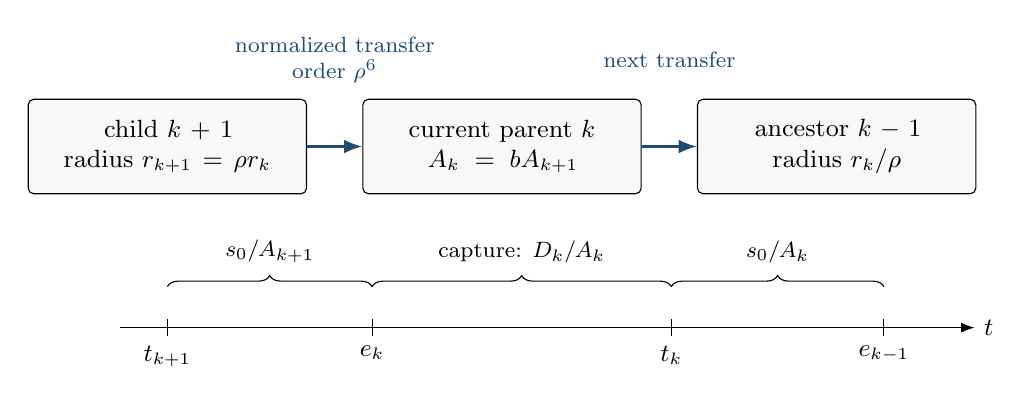
\begin{tikzpicture}[>=Latex,font=\small,
 box/.style={draw,rounded corners=2pt,align=center,minimum height=12mm,
             text width=33mm,fill=cellblue!4}]
 \node[box] (c) at (0,0) {child $k+1$\\radius $r_{k+1}=\rho r_k$};
 \node[box] (p) at (4.25,0) {current parent $k$\\$A_k=bA_{k+1}$};
 \node[box] (a) at (8.5,0) {ancestor $k-1$\\radius $r_k/\rho$};
 \draw[->,thick,cellblue] (c)--(p);
 \draw[->,thick,cellblue] (p)--(a);
 \node[align=center,font=\footnotesize,text=cellblue] at (2.125,1.1)
 {normalized transfer\\order $\rho^6$};
 \node[font=\footnotesize,text=cellblue] at (6.375,1.1) {next transfer};
 \draw[->] (-.6,-2.3)--(10.25,-2.3) node[right] {$t$};
 \draw (0,-2.19)--(0,-2.41) node[below] {$t_{k+1}$};
 \draw (2.6,-2.19)--(2.6,-2.41) node[below] {$e_k$};
 \draw (6.4,-2.19)--(6.4,-2.41) node[below] {$t_k$};
 \draw (9.1,-2.19)--(9.1,-2.41) node[below] {$e_{k-1}$};
 \draw[decorate,decoration={brace,amplitude=4pt}]
 (0,-1.78)--node[above=5pt,font=\footnotesize] {$s_0/A_{k+1}$} (2.6,-1.78);
 \draw[decorate,decoration={brace,amplitude=4pt}]
 (2.6,-1.78)--node[above=5pt,font=\footnotesize] {capture: $D_k/A_k$} (6.4,-1.78);
 \draw[decorate,decoration={brace,amplitude=4pt}]
 (6.4,-1.78)--node[above=5pt,font=\footnotesize] {$s_0/A_k$} (9.1,-1.78);
\end{tikzpicture}
\caption{A finite cascade runs from larger indices to smaller indices.
$t_j$ is the geometric exit of cell $j$,
$e_k\coloneqq t_{k+1}+s_0/A_{k+1}$ is its parent's entrance, and
$D_k\coloneqq A_k(t_k-e_k)=6\sigma^{-1}\log(1/\rho)+O(1)$.
The timeline is schematic and is not drawn to scale.}
\label{fig:cascade}
\end{figure}

There are three points at which a formal instability calculation is
insufficient. First, the growing parent response has a retarded
normalization: an inherited homogeneous component must be estimated,
rather than set to zero. The weighted entrance invariant makes the
parent displacement $O(\rho^{12})$, while the new seed is of order
$\rho^6$. Second, all already activated descendants act on the current
contours. Their support and absolute moments, rather than their contour
norms, give the required forcing bound. Third, a period-map estimate
alone cannot control a crossing between consecutive periods. A
pointwise contour-space forcing estimate supplies a continuous
first-exit argument. These estimates close simultaneously with
constants independent of the finite truncation.

The total capture time is summable because
$\sum_{j\ge0}A_j^{-1}=A_0^{-1}/(1-b)$. A fixed fourth-moment test at
the outer exit detects a nonzero change in the total velocity. Uniform
$W^{1,q}$ bounds and $L^2$ time-Lipschitz bounds then yield convergence
in $C_tL^2_x$, which preserves that departure. Delaying this
nonstationary evolution at the stationary datum gives the family in
Corollary~\ref{intro:refinement}.

\subsection{Dependencies, organization, and notation}
Section~\ref{sec:preliminaries} collects the background tools and
normalizations. Section~\ref{part:bv} supplies bounded-vorticity
realizations and common transport of finite labels.
Section~\ref{part:pc} establishes the unstable cell and local capture;
Section~\ref{part:nt} selects a nonzero transfer.
Sections~\ref{part:cs}--\ref{part:ib} derive support, weighted and
interaction estimates. Sections~\ref{part:re} and~\ref{part:fi} prove
the response estimate and close the finite induction.
Section~\ref{part:cp} proves the main results by compactness.
The final editorial appendices record the changes and the outcome of
the mathematical issue check.
Figure~\ref{fig:dependencies} summarizes the dependencies among these steps.

\begin{figure}[H]
\centering
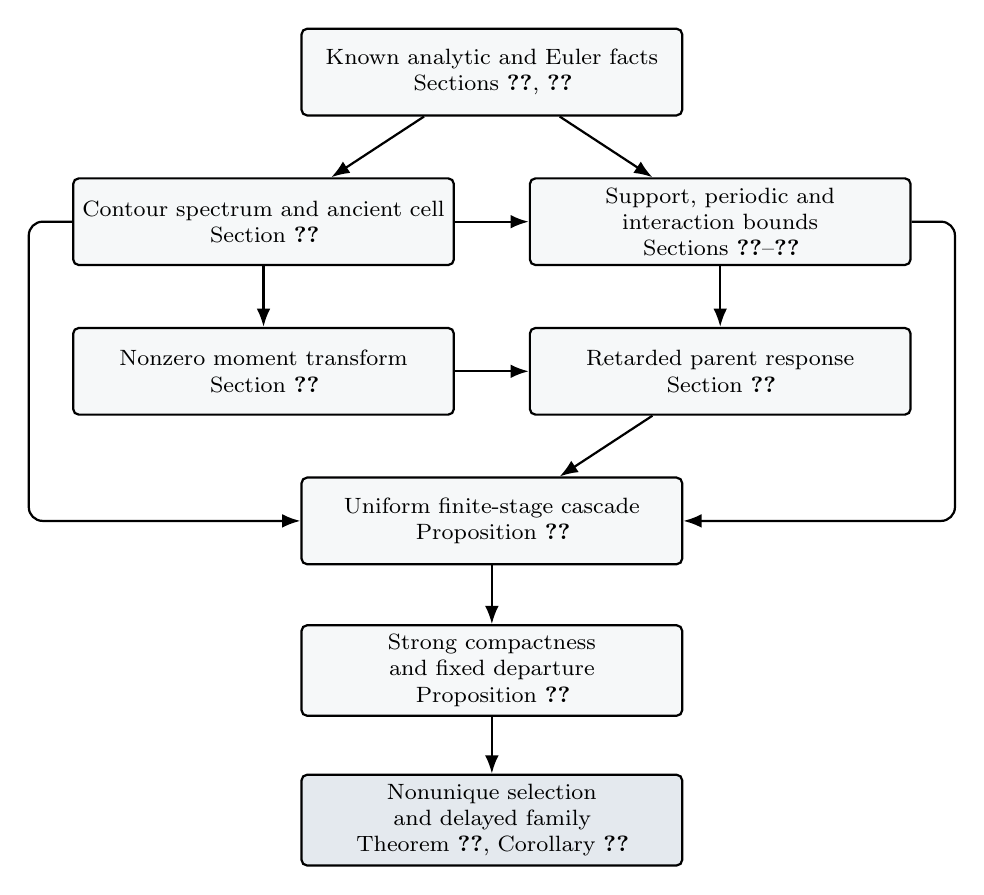
\begin{tikzpicture}[>=Latex,font=\footnotesize,
 dep/.style={draw,rounded corners=2pt,align=center,text width=46mm,
             minimum height=11mm,fill=cellblue!4},
 every path/.style={thick}]
 \node[dep] (pre) at (0,0) {Known analytic and Euler facts\\Sections~\ref{sec:preliminaries}, \ref{part:bv}};
 \node[dep] (cell) at (-2.9,-1.9) {Contour spectrum and ancient cell\\Section~\ref{part:pc}};
 \node[dep] (inter) at (2.9,-1.9) {Support, periodic and interaction bounds\\Sections~\ref{part:cs}--\ref{part:ib}};
 \node[dep] (trans) at (-2.9,-3.8) {Nonzero moment transform\\Section~\ref{part:nt}};
 \node[dep] (response) at (2.9,-3.8) {Retarded parent response\\Section~\ref{part:re}};
 \node[dep] (finite) at (0,-5.7) {Uniform finite-stage cascade\\Proposition~\ref{fi:finite}};
 \node[dep] (limit) at (0,-7.6) {Strong compactness and fixed departure\\Proposition~\ref{cp:limit}};
 \node[dep,fill=cellblue!12] (main) at (0,-9.5) {Nonunique selection and delayed family\\Theorem~\ref{main}, Corollary~\ref{intro:refinement}};
 \draw[->] (pre)--(cell); \draw[->] (pre)--(inter);
 \draw[->] (cell)--(inter);
 \draw[->] (cell)--(trans); \draw[->] (trans)--(response);
 \draw[->] (inter)--(response);
 \draw[->,rounded corners=5pt] (cell.west)--++(-.55,0) |- (finite.west);
 \draw[->] (response)--(finite);
 \draw[->,rounded corners=5pt] (inter.east)--++(.55,0) |- (finite.east);
 \draw[->] (finite)--(limit); \draw[->] (limit)--(main);
\end{tikzpicture}
\caption{The main proof dependencies. The weighted estimate is
conditional on its stated mild-system hypotheses; the interaction
section derives that system for the actual finite Euler solutions.
The simultaneous induction then verifies the hypotheses needed by
the response and capture results.}
\label{fig:dependencies}
\end{figure}

\begingroup\small
\setlength{\tabcolsep}{5pt}
\begin{longtable}{@{}p{.21\textwidth}p{.73\textwidth}@{}}
\caption{Frequently used notation; local definitions appear before use.}
\label{tab:notation}\\
\toprule Symbol & Meaning \\ \midrule
\endfirsthead
\toprule Symbol & Meaning (continued) \\ \midrule
\endhead
\bottomrule\endfoot
$\T,\T^2$ & $\R/2\pi\mathbb Z$ and its square, with Lebesgue measure.\\
$z,\bar z,\mathsf Rx$ & $z\coloneqq x_1+ix_2$, its conjugate, and
$\mathsf Rx\coloneqq x^\perp\coloneqq(-x_2,x_1)$.\\
$K,K_{\T^2}$ & Planar and mean-zero periodic Biot--Savart kernels.\\
$B_r,\mathsf R$ & Disk of radius $r$; a quarter turn denoted by $\mathsf R$.\\
$c^{k,\gamma}$ & Closure of smooth functions in $C^{k,\gamma}$,
$0<\gamma<1$.\\
$[f]_\gamma,\|f\|_r$ & H\"older seminorm and $L^r$ norm.\\
$p,q$ & Prescribed finite exponent and auxiliary exponent
$q>\max\{p,2\}$.\\
$a,W,g_i,d_i$ & Cell radius, cell profile, indicator coefficients
$(g_1,g_2)=(5/2,-3/2)$, and radii $(d_1,d_2)=(a,1)$.\\
$b,\rho,R,A_0$ & Strength ratio, radius ratio, outer radius, and outer strength.\\
$A_j,r_j$ & Strength $A_0b^{-j}$ and radius $R\rho^j$ at scale $j$.\\
$\omega_j,D_{j,i}$ & Transported signed label and its two enclosed domains.\\
$X,\Xi$ & Contour Banach space and fixed-area coordinate chart;
$X(t,s,a)$ denotes the particle flow when time arguments are present.\\
$q_j,Z$ & Norm of an inactive contour coordinate and its weighted maximum.\\
$\sigma,\lambda_*,P$ & Growth rate $9\sqrt{15}/100$, temporal eigenvalue
$\sigma-3i/4$, and material return period $4\pi$.\\
$\lambda,\mathfrak q$ & Expanding multiplier modulus $e^{\sigma P}$
and an adapted complementary bound, $1<\mathfrak q<\lambda$.\\
$\Omega_*,N,F$ & Ancient cell, its conjugate fourth moment, and its
bilateral transform.\\
$J_4(D)$ & Conjugate fourth domain moment $\int_D\bar z^4\,dA$.\\
$\mathcal M(z),\xi(s)$ & Normalized inner-domain moment and its coordinate on
the unstable graph; the exponent $q$ is reserved for integrability.\\
$h,\varepsilon,\Lambda$ & $C_0\rho^6$, $\rho^6$,
and $1+\log(1/\rho)$.\\
$t_k,e_k,s,\tau$ & Exit, entrance, exit-centered child time, and
entrance-centered current time.\\
$N_\rho,Y_\chi,Y_+$ & Actual normalized child moment, retarded full
parent response, and its growing component.\\
$D^+,\log_+$ & Upper right Dini derivative and
$\log_+s\coloneqq\max\{0,\log s\}$.\\
\end{longtable}
\endgroup

We identify vectors with complex numbers in moment and kernel
calculations. Throughout the paper the quarter turn is
\[
 \mathsf R\coloneqq\begin{pmatrix}0&-1\\1&0\end{pmatrix},\qquad
 \mathsf R(x_1,x_2)=(-x_2,x_1).
\] Fourfold symmetry means $\mathsf RD=D$ for sets,
$\omega(\mathsf Rx)=\omega(x)$ for scalar vorticity, and $u(\mathsf Rx)=\mathsf Ru(x)$
for velocity. A label is one fixed signed vorticity component transported
by the common finite Euler flow. Smaller indices denote larger cells.
An ancient solution is defined on every negative time.
Finite products use the maximum norm; empty maxima and sums are zero.
Constants may change from line to line. Independence of the number of
labels is claimed only in estimates where it is proved.

\section{Preliminaries and known results}\label{sec:preliminaries}
This section states the background used in the argument. The
bounded-vorticity theory, singular-integral estimates and
invariant-manifold theorem are existing results. The specific cell,
moment-transfer calculation and uniform cascade estimates are developed
in the subsequent sections.

\subsection{Biot--Savart normalization and elementary analytic tools}
For $x\ne0$ define
\[
 K(x)\coloneqq\frac{x^\perp}{2\pi|x|^2},\qquad
 G_{\R^2}(x)\coloneqq\frac1{2\pi}\log|x|.
\]
On the torus let $G_{\T^2}$ be the distribution uniquely specified by
\[
 \Delta G_{\T^2}=\delta_0-\frac1{4\pi^2},\qquad
 \int_{\T^2}G_{\T^2}=0,\qquad
 K_{\T^2}\coloneqq\nabla^\perp G_{\T^2}.
\]
The first equality specifies its Poisson equation, rather than a
pointwise function. For mean-zero $\omega\in L^r(\T^2)$,
$1<r<\infty$, the velocity $u\coloneqq K_{\T^2}*\omega$ is the unique
mean-zero divergence-free field with curl $\omega$, and
\[
 \|u\|_{W^{1,r}(\T^2)}\le C_r\|\omega\|_{L^r(\T^2)}.
\]
The derivative estimate is the Calder\'on--Zygmund bound
\cite{TaoCZ}; Poincar\'e's inequality supplies the zeroth-order term.
Lemma~\ref{bv:kernel} proves the size, logarithmic-modulus and
far-field bounds in the normalizations used here. The local periodic
decomposition and its higher cancellation are proved in
Section~\ref{cs:torussection}.

We use H\"older's inequality, Minkowski's inequality, and
\[
 \|f\|_p\le\|f\|_1^{\theta}\|f\|_q^{1-\theta},\qquad
 \frac1p=\theta+\frac{1-\theta}{q},\quad 1\le p\le q,
\]
as well as the Sobolev embedding $W^{1,q}(\T^2)\hookrightarrow
C^{0,1-2/q}(\T^2)$ for $q>2$. The latter gives in particular a
bounded continuous representative. On bounded sets, products of
$C^\gamma$ functions satisfy
$[fg]_\gamma\le\|f\|_\infty[g]_\gamma+
\|g\|_\infty[f]_\gamma$.
For a harmonic function on a disk, the interior derivative bounds
\cite[Theorem~2.4]{ABR}, after dilation, take the form
\[
 \|D^mH\|_{L^\infty(B_r)}\le C_m r^{-m}
                       \|H\|_{L^\infty(B_{2r})}.
\]
They are applied only on source-free neighborhoods of target contours.
Scalar integral Gronwall is used with nonnegative locally integrable
coefficients \cite[Lemma~2.7]{Teschl}.

\subsection{Bounded vorticity, contour flows, and invariant manifolds}
For compactly supported planar bounded vorticity of zero circulation,
or mean-zero bounded vorticity on the torus, the normalized Euler
solution is globally unique in the bounded-vorticity class. It has an
area-preserving homeomorphic flow, and its vorticity is transported by
that flow. The signed-data formulation and the precise competitor class
used here are stated and justified in Theorem~\ref{bv:wellposed}, using
\cite{Yudovich1963,CrippaStefani2024}. It follows that finitely many
overlapping or nested indicator labels are transported by one common
flow. Their coefficients are fixed; the labels are not independent
solutions of Euler.

For regular patch boundaries the material contour equation recovers
the Biot--Savart normal velocity. The local analytic formulation is
proved in Lemma~\ref{np:local-general}; Proposition~\ref{np:continuation}
proves the finite signed-family continuation required here.
The corrected version of \cite{Verdera} is a useful reference for
single-patch contour regularity. We do not infer the signed-family
statement solely from a single-patch theorem.

We use \cite[Theorem~1.2]{CFL2003} for a $C^3$ local Banach-space
diffeomorphism. In the application its inverse has invariant splitting
$E_u\oplus E_c$, contracts on the real two-dimensional space $E_u$,
and satisfies the theorem's spectral and nonresonance conditions with
$L=1$. The resulting $C^3$ local graph is unique among $C^2$ locally
invariant graphs tangent to $E_u$. Section~\ref{subsec:unstable-manifold}
checks those hypotheses explicitly after establishing an operator
spectral bound. A Fourier-mode calculation alone would not establish
that bound on the contour Banach space.

\subsection{Time regularity, energy, and strong compactness}
The following consequences are included with proofs to specify the
topology used at the end of the construction.

\begin{lemma}
\label{cp:energy}
Let $T>0$, $q>2$, and let $u$ be a weak Euler solution on
$[0,T]\times\T^2$ satisfying
\[
 u\in C([0,T];L^2(\T^2;\R^2))
       \cap L^\infty(0,T;W^{1,q}(\T^2;\R^2)).
\]
Then
\[
 u\in W^{1,\infty}(0,T;L^2(\T^2;\R^2)),\qquad
 \|\partial_tu\|_{L^\infty(0,T;L^2)}
 \le C_q\|u\|_{L^\infty(0,T;W^{1,q})}^2,
\]
and
\[
 \frac12\|u(t)\|_2^2=\frac12\|u(0)\|_2^2
 \qquad\text{for every }t\in[0,T].
\]
\end{lemma}
\begin{proof}
Sobolev embedding and the orthogonal Leray projection give
\[
 \partial_tu=-\mathbb P((u\cdot\nabla)u),\qquad
 \|\partial_tu\|_{L^\infty_tL^2_x}
 \le C_q\|u\|_{L^\infty_tW^{1,q}_x}^2 .
\]
The Hilbert-space chain rule yields
$\frac{\dd}{\dd t}\|u\|_2^2/2
=-\int u\cdot(u\cdot\nabla u)\dd x=0$.
Spatial mollification justifies the last integration by parts,
using uniform convergence and $W^{1,2}$ convergence.
\end{proof}

\begin{lemma}[Compactness with uniform time control]
\label{pre:compactness}
Let $q>2$, $0<T<\infty$, and
$(v_n)_{n\ge1}\subset C([0,T];L^2(\T^2;\R^2))$.
Assume that there exist $M,L<\infty$ such that
\[
 \sup_{n\ge1}\|v_n\|_{L^\infty(0,T;W^{1,q}(\T^2))}\le M,
 \qquad
 \|v_n(t)-v_n(s)\|_2\le L|t-s|
 \quad(n\ge1,\ s,t\in[0,T]).
\]
Then there exist $v\in C([0,T];L^2(\T^2;\R^2))$ and a strictly
increasing sequence $(n_\ell)_{\ell\ge1}\subset\mathbb N$ such that
\[
 \lim_{\ell\to\infty}\sup_{t\in[0,T]}
       \|v_{n_\ell}(t)-v(t)\|_2=0.
\]
\end{lemma}
\begin{proof}
Continuity in $L^2$ and weak compactness in $W^{1,q}$ extend the
uniform spatial bound to every $t\in[0,T]$. Since $q>2$, this also
bounds the sequence in $H^1$. For the Fourier projection $P_m$ onto
$|k|\le m$, Parseval gives
\[
 \sup_{n,t}\|(I-P_m)v_n(t)\|_2
 \le m^{-1}\sup_{n,t}\|\nabla v_n(t)\|_2\longrightarrow0.
\]
For each $m$, the curves $P_mv_n$ are bounded and equi-Lipschitz in
a finite-dimensional space. Arzel\`a--Ascoli and a diagonal extraction
give uniform convergence of every $P_mv_n$ along one subsequence.
The uniform tail bound then gives convergence in $C([0,T];L^2)$.
\end{proof}



\section{Bounded vorticity and transported domains}\label{part:bv}
\subsection{Kernel estimates and the common flow}\label{bv:section}

Write $M=\R^2$ or $M=\T^2=(\R/2\pi\mathbb Z)^2$. On the
plane let $K(x)=x^\perp/(2\pi|x|^2)$; on the torus let
$\mathcal K=\nabla^\perp G$, where
$\Delta G=\delta_0-|M|^{-1}$ and $\int_MG=0$. Put
$\mathcal K=K$ on the plane. Throughout, $u=\mathcal K*\omega$;
the torus velocity therefore has mean zero. Constants in this
section may depend on the particular finite signed datum and
on the finite time interval, including on its number of labels.

\begin{lemma}
\label{bv:kernel}
There exists $C>0$ such that every
$f\in L^1(\R^2)\cap L^\infty(\R^2)$ satisfies
\begin{align}
 \norm{K*f}_\infty
 &\le C\norm f_1^{1/2}\norm f_\infty^{1/2},\label{bv:speed}\\
 |(K*f)(x)-(K*f)(y)|
 &\le C(\norm f_1+\norm f_\infty)h(1+\log(1/h)),
 \quad h=|x-y|\in(0,\tfrac14].\label{bv:loglip}
\end{align}
For $f\in L^\infty(\T^2)$, the corresponding estimates are
\[
 \|\mathcal K*f\|_\infty\le C\|f\|_\infty,\qquad
 |(\mathcal K*f)(x)-(\mathcal K*f)(y)|
 \le C\|f\|_\infty h(1+\log(1/h)),
\]
where $h=d_{\T^2}(x,y)\in(0,1/4]$.
For each $M\in\{\R^2,\T^2\}$ and $r\in(1,\infty)$, there is
$C_r>0$ such that
\[
 \|\nabla(\mathcal K*f)\|_{L^r(M)}\le C_r\|f\|_{L^r(M)}
 \qquad(f\in L^1(M)\cap L^\infty(M)).
\]
If, in addition, $f\in L^1(\R^2)\cap L^\infty(\R^2)$,
$\operatorname{supp}f\subset B_R$ for some $R>0$, and $\int f=0$,
then
\begin{equation}\label{bv:tail}
 |(K*f)(x)|\le C|x|^{-2}\int_{\R^2}|y|\,|f(y)|\dd y
 \qquad(|x|\ge2R),
\end{equation}
and $K*f\in\bigcap_{1<r<\infty}L^r(\R^2)$.
\end{lemma}
\begin{proof}
For every $a>0$,
\[
 \|K*f\|_\infty\le C(a\|f\|_\infty+a^{-1}\|f\|_1).
\]
Minimization proves \eqref{bv:speed}. Splitting the velocity
difference into distances below $2h$, between $2h$ and $1$, and
above $1$, and using $|DK(z)|\le C|z|^{-2}$, gives
\[
 |(K*f)(x)-(K*f)(y)|
 \le C\|f\|_\infty h+C\|f\|_\infty h\log(1/h)+C\|f\|_1h.
\]
If $\int f=0$ and $|x|\ge2R$, then
\[
 (K*f)(x)=\int_{B_R}[K(x-y)-K(x)]f(y)\,\dd y,
\]
which proves \eqref{bv:tail} and the asserted $L^r$ integrability.
The derivative bound is the Calder\'on--Zygmund estimate
\cite[Corollary~2.10, p.~9]{TaoCZ}. On the torus,
$\mathcal K-K$ is smooth near zero; its derivatives are bounded
on a finite coordinate cover. The same decomposition proves the
periodic estimates.
\end{proof}

\begin{theorem}
\label{bv:wellposed}
Let $M\in\{\R^2,\T^2\}$ and let $\omega_0:M\to\R$ satisfy
\[
 \begin{cases}
 \omega_0\in L^\infty(\R^2),\quad
 \operatorname{supp}\omega_0\subset\subset\R^2,\quad \int_{\R^2}\omega_0=0,
       &M=\R^2,\\
 \omega_0\in L^\infty(\T^2),\quad \int_{\T^2}\omega_0=0,
       &M=\T^2.
 \end{cases}
\]
Set $u_0=\mathcal K*\omega_0$. There exists a global distributional
Euler solution $(u,\omega)$ with $u=\mathcal K*\omega$,
$\omega=\operatorname{curl}u$, $(u,\omega)|_{t=0}=(u_0,\omega_0)$,
and, for every $T>0$ and $r\in(1,\infty)$,
\begin{equation}\label{bv:regularity}
 \begin{split}
 u&\in C([0,T];L^2(M;\R^2))\cap C([0,T];W^{1,r}(M;\R^2)),\\
 \omega&\in C([0,T];L^r(M))\cap L^\infty([0,T]\times M).
 \end{split}
\end{equation}
There is a unique jointly continuous particle flow $X(t,s,a)$,
$s,t\ge0$, satisfying
\[
 \partial_tX(t,s,a)=u(t,X(t,s,a)),\qquad X(s,s,a)=a.
\]
Each $X(t,s,\cdot)$ is an area-preserving homeomorphism,
$X(t,s,\cdot)^{-1}=X(s,t,\cdot)$, and
\begin{equation}\label{bv:transport}
 \omega(t)=\omega_0\circ X(0,t,\cdot),\qquad
 \norm{\omega(t)}_r=\norm{\omega_0}_r
 \quad(t\ge0,\ 1\le r\le\infty).
\end{equation}
For $M=\R^2$,
\[
 \operatorname{supp}\omega_0\subset B_{R_0}
 \ \Longrightarrow\
 \operatorname{supp}\omega(t)\subset B_{R_0+Ut}\quad(t\ge0),\qquad
 U=C\|\omega_0\|_1^{1/2}\|\omega_0\|_\infty^{1/2}.
\]
For each $T>0$, $u$ is unique among distributional Euler velocities
$v=\mathcal K*\operatorname{curl}v$ with initial trace $v(0)=u_0$,
$v\in L^\infty(0,T;L^2(M;\R^2))$, and
\[
 \begin{cases}
 \operatorname{curl}v\in L^\infty(0,T;L^1(\R^2)\cap L^\infty(\R^2)),
       &M=\R^2,\\
 \operatorname{curl}v\in L^\infty((0,T)\times\T^2),&M=\T^2.
 \end{cases}
\]
For every $t_0\in\R$, these assertions hold with $0$ replaced by
$t_0$ and $t$ in the support bound replaced by $t-t_0\ge0$.
\end{theorem}
\begin{proof}
Apply \cite[Theorems~3.3 and~4.1]{CrippaStefani2024} with
$\Theta\equiv1$. The kernel bounds of Lemma~\ref{bv:kernel}
verify Assumption~2.1. Assumption~3.1 holds with $p_0=4$ and
$C_3=0$: convolution is divergence free on
$L^1\cap L^4_{\rm ul}$, and their Theorem~2.2 gives a bounded
continuous velocity. The uniqueness integral diverges and the
corresponding modulus is concave. Thus there is a unique signed
Lagrangian solution with a forward and backward Osgood flow.
Divergence-free approximation and ODE stability imply area
preservation, hence \eqref{bv:transport}. The speed bound gives
the support estimate, and \eqref{bv:tail} gives
$u\in L^\infty(0,T;L^2)$.

Approximation of $\omega_0$ in $L^r$, $r<\infty$, by compactly
supported continuous functions, together with area preservation
and continuity of the flow, yields $\omega\in C_tL^r$.
The derivative estimate gives $\nabla u\in C_tL^r$.
Young's inequality on a common support ball and \eqref{bv:tail}
outside twice that ball give $u\in C_tL^r$, $r>1$; on the torus
Young's inequality suffices. This proves \eqref{bv:regularity}.

Taking the time derivative in the vorticity formulation gives
\begin{equation}\label{bv:timemultiplier}
 \partial_tu=-\mathcal K*\operatorname{div}(u\omega),\qquad
 \|\partial_tu\|_2\le C\|u\omega\|_2.
\end{equation}
The multipliers are, up to sign,
$(\mathsf R\xi)_\ell\xi_j/|\xi|^2$, with zero torus mode set to
zero. For the Leray projection $\mathbb P$, spatial mollification
therefore gives
\[
 \operatorname{curl}\bigl(\partial_tu+\mathbb P(u\cdot\nabla u)\bigr)=0,
 \qquad
 \operatorname{div}\bigl(\partial_tu+\mathbb P(u\cdot\nabla u)\bigr)=0.
\]
The field in parentheses belongs to $L^\infty_tL^2_x$ and is
zero by the Fourier transform on $\R^2$, or by its zero mean on
$\T^2$. This proves the momentum formulation and initial trace.
Conversely, a competitor in the stated class has bounded velocity
and $\nabla u\in L^\infty_tL^2_x$. Mollification justifies taking
the curl of its momentum equation. The resulting weak vorticity
solution is Lagrangian by \cite[Remark~1.7]{CrippaStefani2024},
so their Theorem~4.1 gives uniqueness. Time translation and reversal
give the assertion for an arbitrary initial time.
\end{proof}

\begin{corollary}
\label{bv:labels}
Let $\omega_0=\sum_{j=1}^Nc_j\mathbf1_{D_j^0}$ satisfy the
hypotheses of Theorem~\ref{bv:wellposed}, where $N\in\mathbb N$,
$c_j\in\R$, and each $D_j^0\subset M$ is measurable and is bounded
if $M=\R^2$. Let $X$ be that theorem's flow and set
$D_j(t)=X(t,0,D_j^0)$. Then, for every $j$ and $t\ge0$,
\begin{equation}\label{bv:labeltransport}
 \begin{gathered}
 \mathbf1_{D_j(t)}=\mathbf1_{D_j^0}\circ X(0,t,\cdot),\qquad
 |D_j(t)|=|D_j^0|,\\
 \partial_t\mathbf1_{D_j(t)}+
        \operatorname{div}(u\mathbf1_{D_j(t)})=0
        \quad\text{in }\mathcal D'((0,\infty)\times M).
 \end{gathered}
\end{equation}
For all $a_1,\ldots,a_N\in\R$ and $t\ge0$,
\[
 \sum_{j=1}^Na_j\mathbf1_{D_j(t)}
  =\left(\sum_{j=1}^Na_j\mathbf1_{D_j^0}\right)\circ X(0,t,\cdot),
 \qquad
 D_i^0\subset D_j^0\ \Longrightarrow\ D_i(t)\subset D_j(t).
\]
If $\partial D_i^0$ and $\partial D_j^0$ are compact and disjoint,
then, for every $0<T<\infty$,
\[
 \inf_{t\in[0,T]}\operatorname{dist}(\partial D_i(t),\partial D_j(t))>0.
\]
If $\omega_0\circ\mathsf R=\omega_0$, where $\mathsf R$ is the
quarter turn, then
\[
 u(t,\mathsf Rx)=\mathsf Ru(t,x),\qquad
 X(t,s,\mathsf Ra)=\mathsf RX(t,s,a),\qquad X(t,s,0)=0.
\]
Under this symmetry assumption,
\[
 \mathsf RD_j^0=D_j^0\ \Longrightarrow\ \mathsf RD_j(t)=D_j(t)
 \quad(t\ge0).
\]
Moreover, for every $0<T<\infty$, a compact $\partial D_j^0$ with
$0\notin\partial D_j^0$ satisfies
$\inf_{t\in[0,T]}\operatorname{dist}(0,\partial D_j(t))>0$; if
$D_j^0$ is open and $0\in D_j^0$, there exists $r_{j,T}>0$ such
that $B_{r_{j,T}}\subset D_j(t)$ for all $t\in[0,T]$.
\end{corollary}
\begin{proof}
The transport identities and inclusions follow from bijectivity
and area preservation. For a test function $\phi$,
\[
 \frac{d}{dt}\int_{D_j^0}\phi(t,X(t,0,a))\,\dd a
 =\int_{D_j(t)}(\partial_t\phi+u\cdot\nabla\phi)\,\dd x,
\]
which proves the label equation. For disjoint compact initial
boundaries, continuity and injectivity of $X$ imply
\[
 \min_{\substack{t\in[0,T]\\a\in\partial D_i^0,\ b\in\partial D_j^0}}
       d(X(t,0,a),X(t,0,b))>0.
\]
Kernel covariance and uniqueness give the rotation identities;
$u(t,0)=\mathsf Ru(t,0)$ gives $u(t,0)=0$. The same compactness
argument separates each compact boundary from the fixed origin.
An open set containing the origin therefore contains a uniform
interior disk on $[0,T]$.
\end{proof}

\begin{corollary}
\label{bv:contouridentification}
Let $0<\gamma<1$, $0<T<\infty$, and $g_1,\ldots,g_N\in\R$.
For $j=1,\ldots,N$, let $z_j(t,\cdot)$ be a regular
$C^{1,\gamma}$ Jordan parametrization of $\partial D_j(t)$,
continuous in this norm for $t\in[0,T]$, with pairwise disjoint
images. Define
\[
 \omega(t)=\sum_{j=1}^Ng_j\mathbf1_{D_j(t)},\qquad
 u(t)=\mathcal K*\omega(t).
\]
Assume that $\omega(0)$ satisfies Theorem~\ref{bv:wellposed} and
that, with $n_j$ the unit normal,
\[
 \bigl(\partial_tz_j(t,\theta)-u(t,z_j(t,\theta))\bigr)
       \cdot n_j(t,\theta)=0
 \quad(j=1,\ldots,N,\ t\in[0,T],\ \theta\in\T).
\]
Then, writing $(\omega^{\rm Y},u^{\rm Y},X)$ for the solution and
flow of Theorem~\ref{bv:wellposed} with datum $\omega(0)$,
\[
 D_j(t)=X(t,0,D_j(0)),\qquad
 \omega(t)=\omega^{\rm Y}(t),\qquad u(t)=u^{\rm Y}(t)
 \quad(j=1,\ldots,N,\ t\in[0,T]).
\]
\end{corollary}
\begin{proof}
The bounded signed patch velocity has a unique area-preserving
Osgood flow. The normal-speed equation, after a tangential
reparametrization, transports each boundary and its enclosed
domain by this flow. Thus the signed sum is a Lagrangian
vorticity solution. Uniqueness in Theorem~\ref{bv:wellposed}
identifies its velocity with $u^{\rm Y}$; ODE uniqueness then
identifies every transported domain with $X(t,0,D_j(0))$.
\end{proof}

In particular, for $D_1\subset D_2$, $|D_1|=3\pi/5$ and
$|D_2|=\pi$, the datum
$(5/2)\mathbf1_{D_1}-(3/2)\mathbf1_{D_2}$ has, at every time,
\[
 \int\omega=0,\qquad \norm\omega_\infty=\tfrac32,\qquad
 \norm\omega_1=\frac{6\pi}{5}.
\]
The theorem applies separately to every complete finite signed
sum used below and supplies one common flow for all its labels.
Its bounded-vorticity constants may depend on the truncation;
no uniqueness statement is made for the infinite limit
controlled only in a prescribed finite $L^p$ space.


\section{Contour dynamics and an unstable vortex}\label{part:pc}
\subsection{The contour equation}
For a modern account of the contour Banach-space formulation see the appendix of Verdera \cite{Verdera}. We prove below the operator estimates and the finite-family continuation needed here.

Fix $0<\gamma<1$, $a^2=3/5$, $(d_1,d_2)=(a,1)$ and $(g_1,g_2)=(5/2,-3/2)$. Let
\[
 X=c^{1,\gamma}(\T;\R^2)^2,\qquad z^0_j(\theta)=d_je^{i\theta}.
\]
Here $c^{1,\gamma}$ is the little H\"older space, the closure of smooth functions in $C^{1,\gamma}$. This choice ensures strong continuity of parameter translations. The estimates below are in the ordinary H\"older norm and restrict to this closed subspace by density.
We impose $z_j(\theta+\pi/2)=iz_j(\theta)$ and restrict to the analytic codimension-two submanifold where the enclosed areas are $\pi d_j^2$. The curves are oriented counterclockwise, chord-arc, disjoint, and nested. These conditions hold in a fixed neighborhood of $z^0$. The tangent space of the area constraint consists of variations with zero mean normal component on each circle; tangential variations are unrestricted.

The local area chart may and will be chosen rotation equivariant. Indeed, for $v$ in the kernel of the two linearized area functionals, write $z_i=z_i^0+v_i+c_i(v)z_i^0$ and solve the two area equations for the real scalars $c_i(v)$ by the analytic implicit function theorem. The derivative with respect to each $c_i$ is $2\pi d_i^2\ne0$. The action $G_\vartheta z_i(\theta)=e^{i\vartheta}z_i(\theta-\vartheta)$ fixes $z^0$, preserves areas and this tangent kernel, and therefore satisfies $c_i(G_\vartheta v)=c_i(v)$ by uniqueness. This supplies an equivariant fixed-area chart without using a differentiable quotient by contour reparametrizations.

With $\nabla^\perp=(-\partial_2,\partial_1)$, the contour equation is
\begin{equation}\label{pc:F}
 \dot z_i(\theta)=F_i(z)(\theta)
 =-\frac1{2\pi}\sum_{j=1}^2g_j
 \int_0^{2\pi}\log|z_i(\theta)-z_j(\phi)|\,z'_j(\phi)\,d\phi.
\end{equation}
The minus sign gives $\dot z=iz/2$ for a positive unit disk. The velocity represented by \eqref{pc:F} is the Biot--Savart velocity of $\sum_jg_j\mathbf1_{D_j}$ on each boundary.



The needed differentiability is with respect to the initial contours.
The following operator argument provides it directly.

\begin{lemma}
\label{np:local-general}
Fix $N\in\mathbb N$, $0<\gamma<1$, and $g_1,\ldots,g_N\in\R$.
Set $E_N=C^{1,\gamma}(\T;\R^2)^N$ and
$e_N=c^{1,\gamma}(\T;\R^2)^N$. Let
$\bar z=(\bar z_1,\ldots,\bar z_N)\in E_N$ consist of Jordan
parametrizations satisfying, for some $c,d>0$,
\[
 |\bar z_i(\theta)-\bar z_i(\phi)|
       \ge c\,d_\T(\theta,\phi),\qquad
 \operatorname{dist}(\bar z_i(\T),\bar z_j(\T))\ge d\quad(i\ne j).
\]
Let $F_N$ be the planar contour field \eqref{pc:F} with the sum
taken over $j=1,\ldots,N$. There is a neighborhood $U\subset E_N$
of $\bar z$ such that
\[
 F_N\in C^\omega(U;E_N),\qquad F_N(U\cap e_N)\subset e_N,
\]
and its local flow has $C^3$ dependence on the initial state.
For fixed $N,\gamma,(g_j)$, a bound on $\|z\|_{E_N}$ and positive
lower bounds on $c,d$ give a common positive local lifespan and
common bounds on the first three state derivatives of the flow.
The $C^3$ flow conclusion and these uniform bounds also hold for
\[
 \dot z_i=F_{N,i}(z)+H(t,z_i)
\]
when $H$ is continuous in time with uniformly bounded continuous
spatial derivatives through order five on a fixed neighborhood of
the contours, and after addition of a smooth periodic kernel remainder.
\end{lemma}
\begin{proof}
Complexify the Cartesian components and put $Z^\pm=z^1\pm iz^2$.
Near the fixed reference contour, the quotients
\[
 \mathcal Q^\pm(\theta,\phi)=
 \frac{Z^\pm(\theta)-Z^\pm(\phi)}
      {\bar Z^\pm(\theta)-\bar Z^\pm(\phi)}
\]
satisfy $|\mathcal Q^\pm-1|<1/2$, where bars denote the reference.
The self-interaction logarithm extends holomorphically as
\[
 \log|\bar z(\theta)-\bar z(\phi)|
       +\tfrac12\log\mathcal Q^++\tfrac12\log\mathcal Q^-.
\]
Cross-interaction denominators are separated from zero.

For
\[
 \mathcal C_Zf(\theta)=\operatorname{pv}\int_0^{2\pi}
       \frac{Z'(\phi)f(\phi)}{Z(\theta)-Z(\phi)}\,d\phi,
\]
the kernel and its target derivative have bounds $Cd_\T^{-1}$
and $Cd_\T^{-2}$. Subtracting the principal kernel leaves
$O(d_\T^{\gamma-1})$, and $\mathcal C_Z1=\pm i\pi$.
After subtracting $f(\theta)$, the near and far contributions to
a H\"older difference of size $h$ are bounded by
\[
 C\|f\|_{C^\gamma}h^\gamma,
 \qquad Ch\|f\|_{C^\gamma}\int_{2h}^\pi r^{\gamma-2}\,dr.
\]
Consequently
\begin{equation}\label{pc:cauchyholder}
 \|\mathcal C_Zf\|_{C^\gamma}\le C\|f\|_{C^\gamma}.
\end{equation}
Differentiating the self-interaction of coefficient $g$ gives
\begin{equation}\label{pc:Fderivative}
 \partial_\theta F^\ell(z)
 =-\frac g{4\pi}\sum_{\epsilon\in\{+,-\}}
       (Z^\epsilon)'\mathcal C_{Z^\epsilon}
       \left(\frac{(z^\ell)'}{(Z^\epsilon)'}\right),\qquad\ell=1,2.
\end{equation}
The subtracted integral justifies this identity at $C^{1,\gamma}$
regularity. It also bounds the complexified field in that norm.
Line holomorphy and local boundedness give Banach-valued
holomorphy; the Cauchy coefficient formula applied to derivatives
and H\"older difference quotients bounds its first three derivatives.
Density of smooth contours restricts the field to $c^{1,\gamma}$.

The composition $z_i\mapsto H(t,z_i)$ has three bounded continuous
state derivatives under the stated $C^5$ spatial bounds. Smooth
kernel remainders are nonsingular integrals. The integral equation
and its first three variational equations give the $C^3$ local flow
and the uniform bounds by contraction and Gronwall. In the
applications, $L^1$ continuity of each separated source label gives
time continuity of the external field in these spatial norms.
\end{proof}

\begin{lemma}
\label{pc:regularity}
Let $X=c^{1,\gamma}(\T;\R^2)^2$, let
$z_j^0(\theta)=d_je^{i\theta}$, and let $F$ be given by
\eqref{pc:F}. There exists $r_*>0$ such that
$B_X(z^0,r_*)$ consists of disjoint chord-arc contours and
\[
 F\in C^3(B_X(z^0,r_*);X),\qquad
 \sup_{z\in B_X(z^0,r)}\|D^mF(z)\|_{\mathcal L^m(X;X)}<\infty
 \quad(0<r<r_*,\ m=1,2,3).
\]
The coordinate vector field in the analytic fixed-area chart has
the same $C^3$ regularity and derivative bounds on smaller chart balls.
\end{lemma}
\begin{proof}
Apply Lemma~\ref{np:local-general} to the two reference circles.
The divergence-free velocity preserves the areas, and rotation
equivariance preserves the imposed symmetry.
\end{proof}

\subsection{Continuation of finite families of interfaces}

We give the finite-patch estimates used for continuation directly.
In particular, no general striated-regularity theorem or
same-exponent mollification assertion is needed below. Write
$\mathsf R(x_1,x_2)=(-x_2,x_1)$ and
$K(x)=\mathsf R x/(2\pi|x|^2)$. Off the origin put $k=\nabla K$; thus
\[
 \nabla K=\operatorname{pv}k+\tfrac12\mathsf R\delta_0.
\]
The matrix kernel $k$ is even, homogeneous of degree $-2$, has
zero circular mean, and satisfies $|k(x)|\le C|x|^{-2}$ and
$|\nabla k(x)|\le C|x|^{-3}$.

\begin{lemma}[The two patch estimates]
\label{np:patch-estimates}
Fix $0<\gamma<1$ and let $k=\nabla K$ on $\R^2\setminus\{0\}$.
Let $D\subset\R^2$ be a bounded $C^{1,\gamma}$ Jordan domain with
a defining function $\varphi\in C^{1,\gamma}(\R^2)$ satisfying
\[
 D=\{\varphi>0\},\qquad \varphi<0\text{ on }\R^2\setminus\overline D,
 \qquad \operatorname{supp}\nabla\varphi\subset\subset\R^2.
\]
Set $A=[\nabla\varphi]_\gamma$ and
$m=\inf_{\partial D}|\nabla\varphi|>0$. Then
\begin{equation}\label{np:patch-log}
 \sup_{x\in\R^2,\,\epsilon>0}
 \left|\int_{D\setminus B_\epsilon(x)}k(x-y)\,\dd y\right|
 \le C_\gamma\left(1+|D|+\log_+\frac A m\right),
\end{equation}
and
\[
 \|\nabla(K*\mathbf1_D)\|_\infty
 \le C_\gamma\left(1+|D|+\log_+\frac A m\right).
\]
Let, separately, $\omega\in L^1(\R^2)\cap L^\infty(\R^2)$ be
compactly supported, $v=K*\omega$ with $\nabla v\in L^\infty$,
and $W\in C^\gamma(\R^2;\R^2)\cap L^\infty$ satisfy
$\operatorname{div}(\omega W)=0$ in $\mathcal D'(\R^2)$.
Then $(\nabla v)W$ has the continuous representative
\begin{equation}\label{np:patch-commutator}
 G_W(x)=\int_{\R^2}k(x-y)\omega(y)
                    \bigl(W(x)-W(y)\bigr)\,\dd y,
\end{equation}
and
\begin{equation}\label{np:patch-commutator-bound}
 \begin{split}
 [G_W]_\gamma&\le
 C_\gamma(\|\omega\|_\infty+\|\nabla v\|_\infty)[W]_\gamma,\\
 \|G_W\|_\infty&\le\|\nabla v\|_\infty\|W\|_\infty.
 \end{split}
\end{equation}
The constants $C_\gamma$ depend only on $\gamma$ and the kernel normalization.
\end{lemma}
\begin{proof}
Fix $x$, let $d=\operatorname{dist}(x,\partial D)$, and choose
$z\in\partial D$ with $|x-z|=d$. Put
\[
 n=\frac{\nabla\varphi(z)}{|\nabla\varphi(z)|},\qquad
 \ell=\min\{1,(m/A)^{1/\gamma}\},
\]
with $\ell=1$ if $A=0$. For $\rho<d$, circular cancellation gives
zero contribution. For $\rho\ge d$, Taylor's formula gives
\[
 \varphi(x+\rho\theta)=\nabla\varphi(z)\cdot(x-z+\rho\theta)
                  +O_\gamma(A\rho^{1+\gamma}).
\]
Thus $\mathbf1_D(x+\rho\theta)$ differs from the half-circle
indicator $\mathbf1_{\{n\cdot\theta>0\}}$ only where
\[
 |n\cdot\theta|\le d/\rho+C_\gamma(A/m)\rho^\gamma.
\]
Since $k$ is even with zero circular mean, its integral over a
half-circle vanishes. Hence, when $d<\ell$, the contribution of
$\max\{d,\epsilon\}<\rho<\ell$ is at most
\[
 C_\gamma\int_d^\ell
       \left(\frac d\rho+\frac A m\rho^\gamma\right)
       \frac{\dd\rho}{\rho}\le C_\gamma.
\]
For $d=0$ the first integrand is zero. The remaining contributions
are at most $C|\log\ell|+C|D|$, uniformly in the truncation.
This proves \eqref{np:patch-log}; the principal-value limit and
the term $\mathsf R\mathbf1_D/2$ give the gradient bound.

For $a_r=\mathbf1_{B_r}/(\pi r^2)$, direct radial integration gives
\[
 (K*a_r)(z)=
 \begin{cases}
 \mathsf Rz/(2\pi r^2),&|z|<r,\\
 K(z),&|z|>r.
 \end{cases}
\]
Differentiating and convolving with $\omega$ yields
\begin{equation}\label{np:disk-cancellation}
 \int_{|x-y|>r}k(x-y)\omega(y)\,\dd y
 =(a_r*\nabla v)(x)
       -\frac{\mathsf R}{2\pi r^2}\int_{B_r(x)}\omega(y)\,\dd y.
\end{equation}
All these truncations are bounded by
$\|\nabla v\|_\infty+\|\omega\|_\infty/2$.
Subtracting
$\nabla K*(\omega W)=K*\operatorname{div}(\omega W)=0$
from $(\nabla v)W$ gives \eqref{np:patch-commutator}.
For rough data, regularize $K$ first. The diagonal remainder on
$B_r(x)$ is bounded uniformly by
$C\|\omega\|_\infty[W]_\gamma r^\gamma$, so passage to the
limit identifies the integral with $(\nabla v)W$ at Lebesgue
points; the local delta term cancels.

Let $h=|x-x'|$ and $E=\R^2\setminus B_{2h}(x)$.
The near parts of the H\"older difference are bounded by
$C_\gamma\|\omega\|_\infty[W]_\gamma h^\gamma$.
On $E$, write the difference as
\[
 \begin{split}
 &\int_E[k(x-y)-k(x'-y)]\omega(y)[W(x)-W(y)]\,\dd y\\
 &\quad+[W(x)-W(x')]\int_Ek(x'-y)\omega(y)\,\dd y.
 \end{split}
\]
The first line has modulus at most
\[
 C\|\omega\|_\infty[W]_\gamma h
       \int_{2h}^\infty\rho^{\gamma-2}\,\dd\rho
 \le C_\gamma\|\omega\|_\infty[W]_\gamma h^\gamma.
\]
In the second line, replacing $E$ by
$\R^2\setminus B_{2h}(x')$ changes the integral by at most
$C\|\omega\|_\infty$. Equation~\eqref{np:disk-cancellation}
then gives the seminorm bound and continuity. Equality with
the a.e. product gives the supremum bound.
\end{proof}

\begin{proposition}
\label{np:continuation}
Fix $N\in\mathbb N$, $0<\gamma<1$, bounded Jordan domains
$D_j^0\subset\R^2$, and $g_j\in\R$ satisfying
$\sum_{j=1}^Ng_j|D_j^0|=0$. Suppose that $\partial D_j^0$ admit
pairwise disjoint regular parametrizations
$z_j^0\in c^{1,\gamma}(\T;\R^2)$. Let $X$ be the flow of
Theorem~\ref{bv:wellposed} for
$\omega_0=\sum_jg_j\mathbf1_{D_j^0}$, and define
\[
 D_j(t)=X(t,0,D_j^0),\qquad z_j(t,\theta)=X(t,0,z_j^0(\theta)).
\]
For every $0<T<\infty$ and $j=1,\ldots,N$,
\[
 z_j\in C([0,T];c^{1,\gamma}(\T;\R^2)),\qquad
 \inf_{\substack{t\in[0,T]\\\theta\ne\phi}}
 \frac{|z_j(t,\theta)-z_j(t,\phi)|}{d_\T(\theta,\phi)}>0,
\]
and, for $i\ne j$,
\[
 \inf_{t\in[0,T]}\operatorname{dist}(\partial D_i(t),\partial D_j(t))>0,
 \qquad
 D_i^0\subset D_j^0\ \Longrightarrow\ D_i(t)\subset D_j(t).
\]
For $M=\T^2$, assume that $\bigcup_j\overline{D_j^0}\subset B_r(0)$
and $B_{4r}(0)$ is an injectivity neighborhood. Define
\[
 \tau_r=\inf\left\{t\ge0:
       \bigcup_j\overline{D_j(t)}\not\subset B_r(0)\right\},
 \qquad\inf\varnothing=\infty.
\]
The same regularity and positive lower bounds hold on
$[0,\min\{T,\tau_r\}]$ for every $0<T<\infty$, including $t=\tau_r$
if $\tau_r<\infty$. All bounds may depend on $T$ and the finite initial family.
\end{proposition}
\begin{proof}
Choose defining functions $\varphi_i^0\in C^{1,\gamma}$ with
gradients supported in disjoint boundary neighborhoods and
$\inf_{\partial D_i^0}|\nabla\varphi_i^0|>0$. Such functions
follow from local graph charts, a partition of unity, and constant
extensions away from the boundaries. Along the common flow set
\[
 \varphi_i(t)=\varphi_i^0\circ X(0,t,\cdot),\qquad
 W_i=\mathsf R\nabla\varphi_i.
\]

On an existing compact contour interval,
\eqref{np:patch-log} gives a Lipschitz velocity. Its gradient has
one-sided $C^\gamma$ traces: the Cauchy layers have density
$\overline{Z'}/Z'\in C^\gamma$, and subtracting the density at a
closest boundary point gives the off-boundary derivative bound
\[
 C\int_0^C\frac{s^\gamma}{(d+s)^2}\,\dd s
       \le C_\gamma d^{\gamma-1},\qquad
 d=\operatorname{dist}(x,\partial D).
\]
Integration to the boundary gives an $O(d^\gamma)$ trace error;
comparison through a local graph gives one-sided $C^\gamma$
regularity. Separated layers and smooth remainders are smooth.
The flow Jacobian $M=D_aX(t,0,a)$ consequently satisfies, on
either side of each interface,
\[
 \dot M=\nabla u(t,X)M,\qquad M(0)=I,\qquad\det M=1,
 \qquad \mathsf R\nabla\varphi_i(t,X)=MW_i^0.
\]
Write $W_i^0=\alpha_i\partial_\theta z_i^0$, with
$\alpha_i\in C^\gamma$ nowhere zero. Since
$M_i^\pm\partial_\theta z_i^0=\partial_\theta z_i$,
the two traces of $W_i$ equal
$\alpha_i\partial_\theta z_i$ on its own boundary and vanish
on every other boundary. They therefore glue to a global
$C^\gamma$ field. These preliminary statements concern only
already existing contour intervals.

The fields $W_i$ are divergence free and tangent to every source
boundary. In particular
$\mathbf1_{D_i}W_i=\mathsf R\nabla(\varphi_i)_+$ and
$\operatorname{div}(\omega W_i)=0$ for the signed sum.
The Jacobian identity and \eqref{np:patch-commutator} give
\begin{equation}\label{np:stretching}
 (\partial_t+u\cdot\nabla)W_i=(\nabla u)W_i=G_{W_i}.
\end{equation}
Put
\[
 A_i=[W_i]_\gamma,\quad B_i=\|W_i\|_\infty,\quad
 m_i=\inf_{\partial D_i(t)}|W_i|,\qquad
 \mathcal Q=2+\sum_i(A_i+B_i+m_i^{-1}).
\]
For $v_j=g_jK*\mathbf1_{D_j}$, conservation of area and
\eqref{np:patch-log} imply
\[
 V=\sum_j\|\nabla v_j\|_\infty
 \le C\left(1+\sum_j\log_+\frac{A_j}{m_j}\right)
 \le C(1+\log\mathcal Q).
\]
Here $C$ depends on the fixed finite coefficients, areas, and
$\gamma$. Equation~\eqref{np:stretching} gives, for $s\le t$,
\[
 \begin{gathered}
 B_i(t)\le B_i(s)e^{\int_s^tV},\qquad
 m_i(t)^{-1}\le m_i(s)^{-1}e^{\int_s^tV},\\
 A_i(t)\le e^{\gamma\int_s^tV}A_i(s)
       +\int_s^t e^{\gamma\int_\tau^tV}[G_{W_i}(\tau)]_\gamma\,\dd\tau,
 \qquad [G_{W_i}]_\gamma\le C(1+V)A_i.
 \end{gathered}
\]
These are pointwise characteristic estimates. Scalar Gronwall yields
\begin{equation}\label{np:Qclosure}
 \begin{gathered}
 \|\nabla u\|_\infty\le C(1+\log\mathcal Q),\\
 \mathcal Q(t)\le\mathcal Q(s)
       \exp\left(C\int_s^t(1+\log\mathcal Q(\tau))\,\dd\tau\right),\\
 1+\log\mathcal Q(t)\le(1+\log\mathcal Q(0))e^{Ct}.
 \end{gathered}
\end{equation}

For the torus, fix an interval with all source closures in
$\overline{B_r}$. Uniform continuity of the flow permits the
initial boundary neighborhoods to be chosen so that the transported
gradient supports remain in $B_{2r}$. Extend $W_i$ by zero and the
defining functions by their exterior constants. On $B_{5r/2}$,
\[
 u_{\T}=\sum_jv_j+H,\qquad
 H(t,x)=\sum_jg_j\int_{D_j(t)}(K_{\T^2}-K)(x-y)\,\dd y.
\]
The field $H$ is smooth and divergence free, with fixed spatial
norms bounded by the conserved absolute areas. A cutoff of its
stream function extends it to a global smooth divergence-free
field agreeing with $H$ on $B_{2r}$. For this extension,
\[
 [ (\nabla H)W_i]_\gamma\le C(A_i+B_i),\qquad
 \|(\nabla H)W_i\|_\infty\le CB_i.
\]
Thus \eqref{np:Qclosure} holds with adjusted constants. Outside
$B_{2r}$, source separation bounds the torus gradient. This
argument also applies at a finite first exit, when the closures
still lie in $\overline{B_r}$.

Finally,
\[
 \partial_\theta z_i=\alpha_i^{-1}W_i(t,z_i),\qquad
 [\partial_\theta z_i]_\gamma
 \le\|\alpha_i^{-1}\|_\infty A_i\|\partial_\theta z_i\|_\infty^\gamma
       +[\alpha_i^{-1}]_\gamma B_i.
\]
Hence the material $C^{1,\gamma}$ norms stay bounded on every
finite interval. The finite integral of $\|\nabla u\|_\infty$
gives positive chord-arc and separation constants; the common
homeomorphism preserves nesting. Bounded velocity controls
positions. Lemma~\ref{np:local-general} therefore bounds the
contour vector field up to any finite endpoint. The contours are
Cauchy in $c^{1,\gamma}$ there, retain the geometric lower bounds,
and restart by the local ODE. Corollary~\ref{bv:contouridentification}
identifies this continuation with the common bounded-vorticity flow.
\end{proof}

\subsection{The linearized period map}

\begin{proposition}[Full contour-space spectral splitting]
\label{pc:spectrum}
Let $P=4\pi$, let $\mathcal F$ be the time-$P$ material contour map,
and let $X_0$ be the tangent space at $z^0$ to the fourfold-symmetric
fixed-area contour manifold. Set $L=D\mathcal F(z^0)|_{X_0}$.
There exist closed $L$-invariant real subspaces $E_u,E_c\subset X_0$
such that
\[
 X_0=E_u\oplus E_c,\qquad \dim_\R E_u=2,\qquad
 L|_{E_u}=-e^{\sigma P}I,\qquad
 \operatorname{spr}(L|_{E_c})=1,
\]
where $\sigma=9\sqrt{15}/100$ and $\operatorname{spr}$ denotes
spectral radius. For every $\mu\in(0,\sigma)$ there is $C_\mu<\infty$
such that
\[
 \|(L|_{E_c})^n\|_{\mathcal L(E_c)}\le C_\mu e^{\mu Pn}
 \qquad(n\in\mathbb N\cup\{0\}).
\]
In the relative fourth normal-mode coordinates, $E_u$ is generated
over $\R$ by the complex eigenvector and eigenvalue
\[
 v_+=(1,ia)^{\mathsf T},\qquad
 \lambda_*=\sigma-\frac34i.
\]
\end{proposition}
\begin{proof}
The circular angular velocities are $(\Omega_1,\Omega_2)=(1/2,0)$,
so $P=4\pi$ and $\mathcal F(z^0)=z^0$.
In relative normal coordinates
$r=d_j[1+\Re(\eta_je^{im\theta})]$, linearization gives
\[
 \dot\eta_m=iB_m\eta_m,\qquad
 B_m=\begin{pmatrix}
 \frac54-\frac m2&-\frac34a^{m-2}\\
 \frac54a^{m+2}&-\frac34
 \end{pmatrix}.
\]
This is the reduction of \cite[Section~3]{CFMS} with $c=2/3$,
$(r_1,r_2)=(a,1)$, and vorticity multiplied by $3/2$.
Smooth variation and density identify it with the normal derivative
on the little-H\"older space. Fourfold symmetry allows only
$m\in4\mathbb Z$; fixed areas remove the normal $m=0$ modes.
The discriminant is
\[
 (2-m/2)^2-\tfrac{15}{4}a^{2m}.
\]
For $m=4$, the temporal eigenvalues are
$\pm\sigma-3i/4$, with $\sigma=\sqrt{15}a^4/4$.
The two real multiplier pairs are $-e^{\pm\sigma P}$.
For $m\ge8$, put $d=m/2-2$ and
\[
 \Delta_m=\frac{d-\sqrt{d^2-(15/4)a^{2m}}}{2}
 =\frac{(15/4)a^{2m}}{2(d+\sqrt{d^2-(15/4)a^{2m}})}.
\]
The eigenvalues of $B_m$ are $5/4-m/2+\Delta_m$ and
$-3/4-\Delta_m$, where
\[
 0<\Delta_m\le\tfrac{15}{16}a^{16}<\tfrac14.
\]
Their time-$P$ multipliers are $-e^{\pm4\pi i\Delta_m}$,
uniformly separated from $1$.

Let $L_{\rm n}$ be the normal part of $D\mathcal F(z^0)$.
For $m\ge8$, the eigenvalue corrections are $O(a^{2m}/m)$ and
the eigenvector corrections are $O(a^{m-2}/m)$. Since both
unperturbed time-$P$ phases equal $-1$,
\[
 (L_{\rm n})_m=-I+O(a^{m-2}\operatorname{poly}(m)).
\]
Thus $L_{\rm n}+I$ is exponentially smoothing and compact on
$c^{1,\gamma}$. Away from $-1$, Fredholm's alternative and
Fourier coefficients identify its spectrum with the block
eigenvalues. Removing the expanding fourth-mode pair leaves
spectral radius one. The same argument and separation from $1$
give bounded invertibility of $L_{\rm n}-I$.

Tangential reparametrizations have multiplier $I$, so
\[
 D\mathcal F(z^0)=\begin{pmatrix}L_{\rm n}&0\\C&I\end{pmatrix}.
\]
Changing the tangential coordinate by $C(L_{\rm n}-I)^{-1}$
diagonalizes this block matrix. Hence
$X_0=E_u\oplus E_c$, $\dim_\R E_u=2$, and
\[
 D\mathcal F|_{E_u}=U=-\lambda I,\qquad\lambda=e^{\sigma P},
 \qquad\operatorname{spr}(D\mathcal F|_{E_c})=1.
\]
The spectral-radius formula gives
$\|(D\mathcal F|_{E_c})^n\|\le C_\mu e^{\mu Pn}$ for every
$0<\mu<\sigma$. A weighted supremum of these powers defines an
equivalent norm with complementary one-step bound
$\mathfrak q\in(1,\lambda)$.
\end{proof}

\subsection{The local unstable manifold}
\label{subsec:unstable-manifold}

\begin{proposition}[A strong unstable graph and its continuous invariance]
\label{pc:unstable-graph}
Let $X_0=E_u\oplus E_c$ be the splitting of
Proposition~\ref{pc:spectrum}, and let $\Xi$ be the fixed-area chart.
There exist $r>0$ and
$h\in C^3(B_{E_u}(0,r);E_c)$ with $h(0)=Dh(0)=0$ such that
\[
 \mathcal W^u=\{\Xi(\alpha+h(\alpha)):\alpha\in B_{E_u}(0,r)\}
\]
is locally invariant under $\mathcal F$ and $\mathcal F^{-1}$.
Its germ at $z^0$ is unique among $C^2$ locally invariant graphs
tangent to $E_u$. For
$G_\vartheta z_j(\theta)=e^{i\vartheta}z_j(\theta-\vartheta)$,
\[
 h(G_\vartheta\alpha)=G_\vartheta h(\alpha)
 \qquad(\vartheta\in\R,\ |\alpha|<r).
\]
Let $\Phi_t$ be the material contour flow and set
\[
 R_tz_j(\theta)=z_j(\theta-\Omega_jt),\qquad
 (\Omega_1,\Omega_2)=(1/2,0),\qquad \Psi_t=R_t\Phi_t.
\]
There exist a neighborhood $U_1$ of $z^0$ and $t_0>0$ such that
\[
 \Psi_t(\mathcal W^u\cap U_1)\subset\mathcal W^u
 \qquad(|t|\le t_0).
\]
\end{proposition}
\begin{proof}
Choose the adapted norm with $\mathfrak q<\lambda^{1/4}$.
The map $\mathcal F^{-1}$ is a $C^3$ local diffeomorphism fixing
zero. Its derivative preserves $E_u\oplus E_c$, with
\[
 D\mathcal F^{-1}|_{E_u}=-\lambda^{-1}I,\qquad
 D\mathcal F^{-1}|_{E_c}=(D\mathcal F|_{E_c})^{-1}.
\]
For \cite[Theorem~1.2]{CFL2003}, take $L=1$. Its spectral condition is
\[
 \lambda^{-2}\operatorname{Spec}(D\mathcal F|_{E_c})
       \subset\{|z|\le\lambda^{-2}\}\subset\{|z|<1\};
\]
the nonresonance conditions indexed by $2\le i\le L$ are empty,
and $L+1=2\le3$. The theorem gives the $C^3$ graph $c=h(\alpha)$,
unique among $C^2$ locally invariant graphs tangent to $E_u$.

Set $w=c-h(\alpha)$. Local invariance yields
\begin{align}\label{pc:flatten}
 \alpha^+&=U\alpha+f(\alpha,w),\\
 w^+&=\mathcal C_0w+g(\alpha,w),\nonumber
\end{align}
where $\|\mathcal C_0\|\le\mathfrak q$ and, on a $\delta$-ball,
\[
 \begin{gathered}
 g(\alpha,0)=0,\qquad Df(0)=Dg(0)=0,\\
 |f(\alpha,w)|\le C(|\alpha|+\|w\|)^2,\qquad
 \|g(\alpha,w)\|\le C(|\alpha|+\|w\|)\|w\|.
 \end{gathered}
\]
The rotation action $G_\vartheta$ fixes $z^0$, preserves the
equation and splitting, and acts on $E_u$ by the fourth angular
representation. Graph uniqueness gives the stated equivariance.

Fixed parameter shifts commute with $\Phi_t$. Hence
$\Psi_t=R_t\Phi_t$ is a strongly continuous local group fixing
$z^0$, with $\Psi_P=\mathcal F$ and
$\Psi_t\mathcal F=\mathcal F\Psi_t$. For fixed $t$, its state map
is $C^3$ and its derivative preserves $E_u$. Its image of the
graph is therefore an invariant graph tangent to $E_u$; uniqueness
identifies the germs, as in \cite[Remark~6]{CFL2003}.

To make the neighborhood uniform for $|t|\le t_0$, choose
$\mathfrak q+C\delta<\lambda_0<\lambda$. On a smaller graph,
backward iterates decay as $C\lambda_0^{-n}$. The operators $R_t$
and the local Lipschitz constants of $\Phi_t$ are uniformly
bounded for $|t|\le t_0$, so the images of these iterates have
the same decay. Their flattened complementary coordinates satisfy
\[
 \|w_0\|\le(\mathfrak q+C\delta)^n\|w_{-n}\|
       \le C\left(\frac{\mathfrak q+C\delta}{\lambda_0}\right)^n
       \longrightarrow0.
\]
Thus $w_0=0$ uniformly on one smaller neighborhood. Only state
derivatives at fixed time have been used.
\end{proof}

\subsection{The ancient orbit and its fourth moment}

\begin{proposition}[The ancient cell and its nonzero moment]
\label{pc:ancient-cell}
There exist $\delta_J>0$ and a nonstationary planar Euler vorticity
\[
 \Omega_*(s)=\tfrac52\mathbf1_{D_1(s)}-\tfrac32\mathbf1_{D_2(s)},
 \qquad s\in\R,
\]
satisfying
\[
 \partial_s\Omega_*+(K*\Omega_*)\cdot\nabla\Omega_*=0
       \quad\text{in }\mathcal D'(\R\times\R^2),
\]
such that, for every $s\in\R$,
\[
 D_1(s)\subset D_2(s),\qquad \mathsf RD_i(s)=D_i(s),\qquad
 |D_1(s)|=3\pi/5,\quad |D_2(s)|=\pi,
\]
and $\partial D_i(s)$ have regular $c^{1,\gamma}$ material
parametrizations $z_{*,i}(s)$. With
$(\Omega_1,\Omega_2)=(1/2,0)$ and
$\widetilde z_{*,i}(s,\theta)=z_{*,i}(s,\theta-\Omega_i s)$,
\[
 \|\widetilde z_*(s)-z^0\|_X\le Ce^{\sigma s}\quad(s\le0),
 \qquad |J_4(D_1(0))|=\delta_J.
\]
After fixing this time normalization and one spatial orientation, set
\[
 N(s)=\int_{\R^2}(x_1-ix_2)^4\Omega_*(s,x)\,dx.
\]
There are $c_{\rm anc}\in\C\setminus\{0\}$ and $C<\infty$ such that
\[
 N(s)=c_{\rm anc}\kappa_*e^{\lambda_*s}+O(e^{2\sigma s})
       \quad(s\to-\infty),\qquad
 |N(s)|\le C(1+s)^4\quad(s\ge0),
\]
where $\kappa_*=\pi(\tfrac52a^6-\tfrac32ia)\ne0$.
\end{proposition}
\begin{proof}
Green's formula gives the analytic, reparametrization-invariant
moment functional
\begin{equation}\label{pc:moment-functional}
 J_4(D)=\int_D\bar z^{\,4}\,\dd A(z)
       =\frac1{10i}\int_\T\overline{z(\theta)}^{\,5}z'(\theta)\,\dd\theta.
\end{equation}
Set $\mathcal M(z)=J_4(D_1)/(\pi a^6)$. For the circle variation
$r_j=d_j[1+\Re(\eta_je^{4i\theta})]$,
\[
 \delta J_4(D_j)=\pi d_j^6\eta_j.
\]
Since $v_+=(1,ia)^{\mathsf T}$, the derivative at zero of
$\alpha\mapsto\mathcal M(\Xi(\alpha+h(\alpha)))$ is the identity.
The inverse function theorem therefore parametrizes the graph by
its moment coordinate:
\[
 z(\xi)=\Xi(\alpha(\xi)+h(\alpha(\xi))),\qquad
 \mathcal M(z(\xi))=\xi,\qquad\alpha(\xi)=\xi+O(|\xi|^2).
\]
Because $\mathcal M\circ R_t=\mathcal M$, the moment coordinate
of $\Psi_tz(\xi)$ equals $\mathcal M(\Phi_tz(\xi))$.
Differentiation at time zero gives a $C^2$ finite-dimensional ODE
\[
 \xi'=D\mathcal M(z(\xi))F(z(\xi))
       =\lambda_*\xi+O(|\xi|^2),\qquad\lambda_*=\sigma-3i/4.
\]
Moreover,
\[
 \mathcal M(G_\vartheta z)=e^{-4i\vartheta}\mathcal M(z),\qquad
 (|\xi|)'=\sigma|\xi|+O(|\xi|^2)>0
\]
for sufficiently small nonzero $\xi$. Every nonzero local orbit
meets a fixed small moment circle; rotation is transitive on
that circle. ODE uniqueness identifies these orbits up to time
translation and one fixed rotation. The corresponding material
identity is
\begin{equation}\label{pc:material-identification}
 \Phi_tG_\vartheta\Psi_sz=G_\vartheta R_s\Phi_{t+s}z.
\end{equation}
Thus the material shifts and spatial rotation are constant in time.

Choose one orbit with $|J_4(D_1(0))|=\delta_J$ and fix its
orientation. Backward integration gives
$|\xi(s)|\le Ce^{(\sigma-\eta)s}$ for $0<\eta<\sigma/2$.
Since $\xi(s)\ne0$,
\[
 e^{-\lambda_*s}\xi(s)=\xi(0)
 \exp\left(-\int_s^0
       \frac{\xi'(t)-\lambda_*\xi(t)}{\xi(t)}\,\dd t\right).
\]
The integrand is $O(|\xi(t)|)$ and integrable at $-\infty$.
Hence $e^{-\lambda_*s}\xi(s)$ has a nonzero limit
$c_{\rm anc}$. It follows first that $|\xi(s)|\le Ce^{\sigma s}$,
then that the omitted integral on $(-\infty,s]$ is $O(e^{\sigma s})$.
Consequently
\[
 \xi(s)=c_{\rm anc}e^{\lambda_*s}+O(e^{2\sigma s}).
\]

The associated nested patch extends to all finite times by
Theorem~\ref{bv:wellposed} and Proposition~\ref{np:continuation}.
Transport preserves its symmetry, areas, and
\[
 \int\Omega_*=0,\qquad\|\Omega_*\|_\infty=\tfrac32,
 \qquad\|\Omega_*\|_1=\tfrac{6\pi}{5}.
\]
Its negative-time supports are bounded by the local graph.
Lemma~\ref{bv:kernel} gives bounded speed, so
$\operatorname{supp}\Omega_*(s)\subset B_{C(1+s)}$ for $s\ge0$,
and $|N(s)|\le C(1+s)^4$.
For the domains enclosed by $z(\xi)$,
\[
 \tfrac52J_4(D_1)-\tfrac32J_4(D_2)
       =\kappa_*\xi+O(|\xi|^2),\qquad
 \kappa_*=\pi(\tfrac52a^6-\tfrac32ia)\ne0.
\]
Therefore
\begin{equation}\label{pc:ancient-moment}
 N(s)=c_{\rm anc}\kappa_*e^{(\sigma-3i/4)s}+O(e^{2\sigma s}).
\end{equation}
Theorem~\ref{nt:thm:laplace} now applies to this orbit.
\end{proof}

\subsection{Forced passage near the unstable orbit}
We first give the discrete estimate in fixed-time coordinates. Its continuous geometric version is stated separately below with an explicit pointwise forcing hypothesis. They are directly applicable to a parent contour forced by separated interior vorticity: the external velocity is harmonic on a fixed neighborhood of the parent interfaces, so its $C^{2,\gamma}$ norm controls its contribution to the contour map.

Let $\varepsilon\downarrow0$. Over consecutive intervals of length $P$, assume the external velocity induces map errors bounded by
\begin{equation}\label{pc:force}
 |r^\alpha_n|+\norm{r^w_n}
 \le \varepsilon K(1+n)^M
       +\kappa_\varepsilon (|\alpha_n|+\norm{w_n}),
 \qquad
 \kappa_\varepsilon\log(1/\varepsilon)\longrightarrow0.
\end{equation}
Fixed-time variation of constants and Lemma~\ref{pc:regularity} give this map bound whenever the analogous external-velocity bounds hold on each interval. A fixed enlargement of $K$ absorbs the bounded flow over one period. The $\kappa_\varepsilon$ term allows small state-proportional outer feedback; it cannot replace a large additive error.

Suppose at the entry section
\[
 \alpha_0=\varepsilon A_0,\quad
 \norm{w_0}\le\varepsilon W_0,
 \qquad H:=|A_0|>0,
\]
and choose the entry far enough along the linear response that
\begin{equation}\label{pc:margin}
 K\sum_{n\ge0}\lambda^{-n-1}(1+n)^M\le H/16,
 \qquad W_0\le c_* H.
\end{equation}
Here $c_*>0$ is a sufficiently small fixed cone constant. Both conditions can follow from an exponentially growing response with only polynomial forcing and complementary growth strictly below $\sigma$. In an application, the convergence of the actual entry data to this response must include the entire earlier history.

We first estimate the completed period maps.

\begin{proposition}
\label{pc:capture}
Let $(\alpha_n,w_n)$ be the flattened coordinates of forced
two-interface Euler contours at times $nP$. Assume
\eqref{pc:force},
\[
 \alpha_0=\varepsilon A_0,\qquad \|w_0\|\le\varepsilon W_0,
 \qquad H=|A_0|>0,
\]
and the entrance inequalities \eqref{pc:margin}, with
$A_0,W_0,K,M$ fixed independently of $\varepsilon$.
There exist $\delta,C,\eta,\varepsilon_0>0$, depending only on
the reference patch and these fixed bounds, such that, for
$0<\varepsilon<\varepsilon_0$, the index
\[
 n_\varepsilon=\min\{n\in\mathbb N\cup\{0\}:|\alpha_n|\ge\delta\}
\]
is finite, all preceding iterates remain in the local chart, and
\[
 \left|n_\varepsilon-
        \frac{\log(1/\varepsilon)}{\log\lambda}\right|\le C,
 \qquad
 \|w_{n_\varepsilon}\|\le
        C\varepsilon^\eta+C\kappa_\varepsilon\delta.
\]
\end{proposition}
\begin{proof}
Choose $\delta$ so that
$\mathfrak q_\delta=\mathfrak q+2C\delta<\lambda^{1/2}$,
then take $\varepsilon$ so that $\kappa_\varepsilon\le C\delta$.
Under the provisional cone and amplitude bounds, the second
equation of \eqref{pc:flatten} gives
\begin{equation}\label{pc:wbound}
 \|w_n\|\le C\varepsilon\mathfrak q_\delta^n
       +C\kappa_\varepsilon|\alpha_0|\lambda^n.
\end{equation}
Here the additive and state-proportional sums satisfy
\[
 \sum_{j<n}\mathfrak q_\delta^{n-1-j}(1+j)^M
       \le C_M\mathfrak q_\delta^n,\qquad
 \sum_{j<n}\mathfrak q_\delta^{n-1-j}\lambda^j\le C\lambda^n.
\]
For the cone estimate use the sharper inequality
\[
 \lambda^{-n}\sum_{j<n}\mathfrak q_\delta^{n-1-j}(1+j)^M
       \le\sum_{j<n}\lambda^{-j-1}(1+j)^M.
\]
By \eqref{pc:margin}, the normalized additive contribution is
at most $1/8$. With $c_*\le1/32$, the initial contribution is
at most $1/16$; the remaining contribution is
$C\kappa_\varepsilon$. Thus the cone $\|w_n\|\le|\alpha_n|/4$
is strictly improved for small $\varepsilon$.

Multiplying the first equation by $U^{-n}$ and summing yields
\[
 |U^{-n}\alpha_n-\alpha_0|
 \le\frac{|\alpha_0|}{16}
       +C(\delta+\kappa_\varepsilon n)|\alpha_0|,
\]
because
\[
 \sum_{j<n}\lambda^{-j-1}|\alpha_j|^2
       \le C\delta|\alpha_0|.
\]
For $n\le C\log(1/\varepsilon)$, the right side is less than
$|\alpha_0|/2$ after fixing $\delta$ and then $\varepsilon$.
Hence
\[
 \tfrac12|\alpha_0|\lambda^n\le|\alpha_n|
       \le2|\alpha_0|\lambda^n.
\]
Start with strict, slightly wider bounds and choose the section
with room for the bounded one-step overshoot. First exit then
occurs at $n_\varepsilon=\log(1/\varepsilon)/\log\lambda+O(1)$,
within the logarithmic range just used. Substitution into
\eqref{pc:wbound} gives
\[
 \|w_{n_\varepsilon}\|
 \le C\varepsilon^{1-\log\mathfrak q_\delta/\log\lambda}
       +C\kappa_\varepsilon\delta,
\]
with exponent greater than $1/2$.
\end{proof}

\subsubsection{Passage through a geometric section}
\label{pc:continuous-section}

Proposition~\ref{pc:capture} is a statement about completed period
maps. Continuous capture uses the following additional, pointwise
hypothesis. We state it in the same fixed-area contour space, not merely
for a selected Fourier coefficient.

Use the bounded value rotations
\[
 S_t(z_1,z_2)=(e^{it/2}z_1,z_2),\qquad w=S_{-t}z,
\]
and write $w=\Xi(x)$ in the fixed-area chart. The unforced equation
becomes $\dot x=\mathcal G(t,x)$, where $\mathcal G(t,0)=0$,
$\mathcal G$ is $P$-periodic, and its first two derivatives in $x$
are uniformly bounded on one fixed chart. This follows by substituting
the bounded operators $S_t$ into the contour equation; no derivative
of a parameter-translation group is involved. A different starting
phase gives the same bounds. The exact phase identities are recorded
in \eqref{ib:phase-conjugacy}.

Let $\mathcal U(t,s)$ be the linear propagator at $x=0$ and set
$\lambda_* =\sigma-3i/4$. Its growing real two-dimensional bundle has
a complex coordinate $y(t)$ whose linear propagation is
$e^{\lambda_*(t-s)}$. Normalize it so that $y(nP)=\alpha_n$.
Write $\zeta(t)=P_c(t)x(t)$ for the complementary linear projection.
For any fixed $0<\mu<\sigma/4$, the full monodromy calculation gives
\begin{equation}\label{pc:continuous-linear}
 \norm{\mathcal U(t,s)P_c(s)}\le B e^{\mu(t-s)},\qquad
 B^{-1}\norm{x(t)}\le |y(t)|+\norm{\zeta(t)}\le B\norm{x(t)}.
\end{equation}
Here and below $B$ can be enlarged by fixed chart constants.
For completeness, $P_c(t)=\mathcal U(t,0)P_c(0)\mathcal U(0,t)$ is
periodic because $P_c(0)$ commutes with the monodromy. Choose the
embedding $\mathcal L_u(0):\C\to E_u$ with the fourth-normal-mode
normalization used for $\alpha$, and put
\[
 \mathcal L_u(t)=\mathcal U(t,0)\mathcal L_u(0)e^{-\lambda_*t},
 \qquad y(t)=\mathcal L_u(t)^{-1}(I-P_c(t))x(t).
\]
The identity $\mathcal U(P,0)|_{E_u}=-\lambda I=e^{\lambda_*P}I$
makes this frame periodic and proves the stated scalar propagation
and the equality $y(nP)=\alpha_n$. Complete-period bounds and bounded
evolution for the two remaining fractional periods give
\eqref{pc:continuous-linear}. At integer periods,
$\zeta(nP)=h(\alpha_n)+w_n$, so its difference from the flattened coordinate
is quadratic in $\alpha_n$.

Fix $M\ge0$ and $K_c\ge0$. Suppose the actual contour equation has a
continuous, contour-space-valued perturbation on its interval of
existence and satisfies
\begin{equation}\label{pc:pointwise}
 \dot x=\mathcal G(t,x)+\mathfrak f_\varepsilon(t),\qquad
 \norm{\mathfrak f_\varepsilon(t)}
 \le \varepsilon K_c(1+t)^M
       +\widehat\kappa_\varepsilon\norm{x(t)},\qquad
 \widehat\kappa_\varepsilon\log(1/\varepsilon)\longrightarrow0.
\end{equation}
The inequality is required at every time at which the local
bounds are being used. It may be verified on a provisional common
first-exit interval. $K_c$ and the local-flow constants are independent
of $\varepsilon$ and of the number of other blocks. The perturbation
preserves the fixed-area chart, as it does for the actual divergence-free
Euler external field.

Define the finite constants
\[
 I_M=\int_0^\infty e^{-\sigma s}(1+s)^M\,ds,\qquad
 S_M=\sum_{n\ge0}\lambda^{-n-1}(1+n)^M.
\]
There is a fixed $C_{\rm map}$ such that
\eqref{pc:pointwise}, on a completed period within the local envelope,
implies \eqref{pc:force} with
\begin{equation}\label{pc:pointwise-to-map}
 K=C_{\rm map}K_c,\qquad
 \kappa_\varepsilon=C_{\rm map}\widehat\kappa_\varepsilon.
\end{equation}
Indeed the Duhamel estimate on that period bounds the difference of
the forced and unforced endpoint maps by a fixed constant times the
integral of $\norm{\mathfrak f_\varepsilon}$. On a provisional
exponential envelope, $\sup_{[nP,(n+1)P]}\norm{x}$ is bounded by a
fixed multiple of $|\alpha_n|+\norm{w_n}$; the polynomial is bounded by
$(1+P)^M(1+n)^M$. The fixed change to flattened coordinates only
enlarges this constant. This deduction is used only after that period
has actually been completed.

Choose a fixed small cone aperture $\vartheta>0$ and then a fixed
constant $C_{\rm cap}$ large enough for the linear, chart, and
fractional-period bounds below. In addition to \eqref{pc:margin},
with \eqref{pc:pointwise-to-map}, impose the strict continuous margins
\begin{equation}\label{pc:continuous-margin}
 \frac{C_{\rm cap}K_c I_M}{H}<\frac{\vartheta}{16},\qquad
 \frac{C_{\rm cap}W_0}{H}<\frac{\vartheta}{16}.
\end{equation}
All these constants are fixed before choosing the entry far along the
retarded response. Exponential growth of $H$ and smaller complementary
growth allow these strengthened, fixed margins whenever $K_c$ grows
only polynomially in that entry time. Uniform strict inequalities are
preserved by a sufficiently small fixed error in normalized entry data.

We now locate the first passage through the geometric section.

\begin{proposition}
\label{pc:continuous-capture}
Let $x_\varepsilon$ satisfy \eqref{pc:pointwise} and have entrance
data $\alpha_0=\varepsilon A_0$, $\|w_0\|\le\varepsilon W_0$,
$H=|A_0|>0$. Assume \eqref{pc:margin} and
\eqref{pc:continuous-margin}, with the constants related by
\eqref{pc:pointwise-to-map}. There exist a chart radius $\delta>0$,
a section size $\delta_J>0$, and $C,\varepsilon_0>0$, independent of
$\varepsilon$, such that, for $0<\varepsilon<\varepsilon_0$,
\[
 t_\varepsilon=\inf\{t\ge0:|J_4(D_1(t))|=\delta_J\}<\infty,
 \qquad J_4(D)=\int_D\bar z^{\,4}\,\dd A(z),
\]
\[
 \left|t_\varepsilon-\sigma^{-1}\log(1/\varepsilon)\right|\le C,
 \qquad
 \left.\frac{d}{dt}|J_4(D_1(t))|\right|_{t=t_\varepsilon}>0.
\]
Let $z_\varepsilon(t)$ be the corresponding material contour pair.
There exist a spatial rotation and material parameter shifts,
constant in time, sending the canonical section contour $z_*(0)$
to a contour $\widehat z_*(0)$ such that
\begin{equation}\label{pc:continuous-reset}
 \begin{split}
 \|z_\varepsilon(t_\varepsilon)-\widehat z_*(0)\|_X
 &\le C\left[\varepsilon^{\eta_d}
  +\varepsilon K_c(1+\log(1/\varepsilon))^M
  +\widehat\kappa_\varepsilon\delta\right],\\
 \eta_d&=1-\frac{\log\mathfrak q_\delta}{\log\lambda}>\frac12.
 \end{split}
\end{equation}
The comparison uses the same rotating frame for both contours.
Set $E_\varepsilon(t)=\varepsilon H e^{\sigma t}$. On every
provisional interval $[0,t_*]\subset[0,t_\varepsilon]$ satisfying
the loose bounds \eqref{pc:continuous-bootstrap}, these bounds improve to
\[
 \tfrac34E_\varepsilon(t)\le|y(t)|\le\tfrac54E_\varepsilon(t),\qquad
 \|\zeta(t)\|\le\tfrac12\vartheta E_\varepsilon(t)
 \quad(0\le t\le t_*).
\]
The constants are uniform for $H$ in a fixed compact subset of
$(0,\infty)$ and for uniform strict entrance margins.
\end{proposition}

\begin{proof}
Use $E_\varepsilon(t)=\varepsilon H e^{\sigma t}$ from the
statement and put
$\mathcal R(t,x)=\mathcal G(t,x)-D_x\mathcal G(t,0)x$.
The $C^2$ bound gives $\|\mathcal R(t,x)\|\le C\|x\|^2$.
On any existing interval $[0,t_*]$ with
$t_*\le\sigma^{-1}\log(1/\varepsilon)+C_+$, impose
\begin{equation}\label{pc:continuous-bootstrap}
 \tfrac12E_\varepsilon(t)\le|y(t)|\le2E_\varepsilon(t),\qquad
 \|\zeta(t)\|\le\vartheta E_\varepsilon(t),\qquad\|x(t)\|\le\delta.
\end{equation}
Then $\|x(t)\|\le CE_\varepsilon(t)$,
$E_\varepsilon(t)\le C\delta$, and
$\|\zeta(0)\|\le\varepsilon W_0+C\varepsilon^2H^2$.
For every $t\le t_*$,
\begin{align}\label{pc:continuous-weighted}
 \frac1{|\alpha_0|}\int_0^t e^{-\sigma s}
       \|\mathfrak f_\varepsilon(s)\|\,ds
 &\le\frac{K_cI_M}{H}+C\widehat\kappa_\varepsilon t,\\
 \frac1{|\alpha_0|}\int_0^t e^{-\sigma s}
       \|\mathcal R(s,x(s))\|\,ds
 &\le C|\alpha_0|\int_0^t e^{\sigma s}\,ds\le C\delta.\nonumber
\end{align}
Projection of Duhamel's formula gives
\begin{equation}\label{pc:continuous-growing}
 \frac{|e^{-\lambda_*t}y(t)-\alpha_0|}{|\alpha_0|}
 \le C\left(\frac{K_cI_M}{H}+\widehat\kappa_\varepsilon t+\delta\right),
\end{equation}
and the complementary propagator gives
\begin{equation}\label{pc:continuous-complement}
 \frac{\|\zeta(t)\|}{E_\varepsilon(t)}
 \le B\left[\frac{W_0}{H}+C\varepsilon H
       +C\left(\frac{K_cI_M}{H}+\widehat\kappa_\varepsilon t+\delta\right)
       \right].
\end{equation}
The strict margins, followed by small $\delta$ and $\varepsilon$,
therefore imply
\[
 \tfrac34E_\varepsilon(t)\le|y(t)|\le\tfrac54E_\varepsilon(t),\qquad
 \|\zeta(t)\|\le\tfrac12\vartheta E_\varepsilon(t).
\]
At grid times these bounds also imply the flattened cone, since
$h(\alpha)=O(|\alpha|^2)$.

The first variation of $J_4$ on the growing bundle is
$\pi a^6\eta_1$, up to a unit material-phase factor. Consequently
\begin{equation}\label{pc:continuous-moment-comparison}
 c_J|y(t)|\le|J_4(D_1(t))|\le C_J|y(t)|,\qquad
 \|x(t)\|\le C|y(t)|.
\end{equation}
Choose $\delta_J$ so that $|J_4|\le\delta_J$ implies
$\|x\|<\delta/2$ inside the cone. Every provisional endpoint
below the section then retains strict cone and chart bounds and
extends by local existence. The two moment bounds give
\[
 \sigma^{-1}\log(1/\varepsilon)-C_-
       \le t_\varepsilon\le\sigma^{-1}\log(1/\varepsilon)+C_+.
\]
All these estimates hold on truncated intervals, including
endpoints between consecutive periods.

Let $nP<t_\varepsilon\le(n+1)P$; for a grid crossing take the
preceding grid point. Only completed periods are used in
\eqref{pc:wbound}, which gives
\[
 \|w_n\|\le C\varepsilon^{\eta_d}
       +C\widehat\kappa_\varepsilon\delta.
\]
Let $\widetilde x$ be the unforced orbit starting at $nP$ on
the unstable graph with coordinate $\alpha_n$, in the same fixed
material phase. For $0\le s\le t_\varepsilon-nP$,
\begin{equation}\label{pc:fractional-comparison}
 \begin{split}
 \|x(nP+s)-\widetilde x(s)\|
 &\le C_P\left(\|w_n\|+
       \int_0^s\|\mathfrak f_\varepsilon(nP+r)\|\,dr\right)\\
 &\le C\left[\varepsilon^{\eta_d}
       +\varepsilon K_c(1+\log(1/\varepsilon))^M
       +\widehat\kappa_\varepsilon\delta\right]\longrightarrow0.
 \end{split}
\end{equation}
The unforced orbit is a fixed rotation and material shift of the
canonical orbit. Near its section,
\[
 \frac{d}{dt}|J_4|=\sigma|J_4|+O(|J_4|^2)\ge c_*>0.
\]
Analyticity of the moment functional in the physical contours gives
\[
 \left|\frac{d}{dt}|J_4(x)|-\frac{d}{dt}|J_4(\widetilde x)|\right|
 \le C\left(\|x-\widetilde x\|+\|\mathfrak f_\varepsilon\|\right).
\]
Thus the actual slope is at least $c_*/2$ in the terminal section
band. Continuity gives the same bound at the first crossing.
The positive unforced slope bounds the difference of section times
by the right side of \eqref{pc:fractional-comparison}, proving
\eqref{pc:continuous-reset}. This comparison follows one unforced
trajectory with one fixed alignment. The constants are uniform
for $H$ in a fixed compact subset of $(0,\infty)$ and uniform
strict entrance margins.
\end{proof}

Section~\ref{part:fi} verifies \eqref{pc:pointwise} for the actual
Euler contours and applies Proposition~\ref{pc:continuous-capture}.
Its reset error depends on the current forcing and entrance margins.


\section{A nonzero fourth-moment response}\label{part:nt}
\subsection{The bilateral transform and a finite dominance time}

\begin{theorem}
\label{nt:thm:laplace}
Let $\sigma,\delta>0$, $\nu\in\R$, $d\ge0$, and
$\kappa\in\C\setminus\{0\}$. Suppose
$N\in L^1_{\rm loc}(\R;\C)$ satisfies, for some $C<\infty$,
\[
 |N(s)-\kappa e^{(\sigma+i\nu)s}|\le Ce^{(\sigma+\delta)s}
       \quad(s\le s_-),\qquad
 |N(s)|\le C(1+s)^d\quad(s\ge0),
\]
where $s_-<0$. On $S_\sigma=\{z\in\C:0<\Re z<\sigma\}$,
the integral
\[
 F(z)=\int_\R e^{-zs}N(s)\,\dd s
\]
converges absolutely and satisfies $F\in\mathcal O(S_\sigma)$ and
$F\not\equiv0$. For every $\beta\in\R$ and
$0<b_1<b_2<1$,
\[
 \#\{b\in[b_1,b_2]:F(b(\sigma+i\beta))=0\}<\infty.
\]
\end{theorem}
\begin{proof}
Put $z_0=\sigma+i\nu$ and subtract the leading exponential on
$(-\infty,0]$. The remainder and the positive-time integral define
a holomorphic $H$ on $0<\Re z<\sigma+\delta$, and
\[
 F(z)=\frac{\kappa}{z_0-z}+H(z)\qquad(0<\Re z<\sigma).
\]
If $F$ vanished identically, the identity theorem applied to
$\kappa+(z_0-z)H(z)$ on the larger strip would give $\kappa=0$
at $z=z_0$. The isolated-zero theorem gives the last assertion.
\end{proof}

A fixed time translation and rotation multiply $F$ by
$e^{i\vartheta-zs_*}$ and therefore do not change its zeros.
The transform depends on the full isolated continuation, but it
will only be used to choose a finite observation time.

\begin{theorem}
\label{nt:thm:survival}
Let $N,F,\sigma,\nu,d$ satisfy Theorem~\ref{nt:thm:laplace}, and
fix $\lambda=\sigma+i\nu$, $K\in\C\setminus\{0\}$,
$\varpi\in\R$, and $b\in(0,1)$ such that
$F_b=F(b(\lambda+i\varpi))\ne0$. Define
\begin{equation}\label{nt:eq:Y}
 Y(s)=K e^{b\lambda s}\int_{-\infty}^s
                  e^{-b(\lambda+i\varpi)t}N(t)\,\dd t.
\end{equation}
For every $B>0$ and $\epsilon\in(0,1/2)$, there exists
$s_0=s_0(N,b,\lambda,K,\varpi,B,\epsilon)\ge0$ with $Y(s_0)\ne0$
such that the following holds for every $S>s_0$:
if $f\in L^1([s_0,S];\C)$ and
$\widetilde Y\in W^{1,1}([s_0,S];\C)$ satisfy
\[
 \widetilde Y'=b\lambda\widetilde Y+f\quad\text{a.e.},\qquad
 |f(s)|\le B(1+s)^d\quad\text{a.e.},\qquad
 |\widetilde Y(s_0)-Y(s_0)|\le\epsilon|Y(s_0)|,
\]
then
\begin{equation}\label{nt:eq:lowerbound}
 |\widetilde Y(s)|\ge
 (1-2\epsilon)|Y(s_0)|e^{b\sigma(s-s_0)}
 \qquad(s\in[s_0,S]).
\end{equation}
\end{theorem}
\begin{proof}
The exponential tail estimate gives
$Y(s)=KF_be^{b\lambda s}+O((1+s)^d)$ for $s\ge0$.
Choose $s_0$ with
\[
 B\int_0^\infty e^{-b\sigma t}(1+s_0+t)^d\dd t
                       \le\epsilon|Y(s_0)|.
\]
Variation of constants implies that
$e^{-b\lambda(s-s_0)}\widetilde Y(s)$ differs from $Y(s_0)$
by at most $2\epsilon|Y(s_0)|$.
\end{proof}

The retarded normalization is
$e^{-b\lambda s}Y(s)\to0$ as $s\to-\infty$.
The unweighted condition $Y(s)\to0$ would allow an arbitrary
homogeneous component. Section~\ref{part:re} bounds the actual
inherited component before using this response.

\subsection{The exact fourth-mode coefficient}
For a real, fourfold-symmetric, zero-circulation vorticity
supported in $B_L$, define
\[
 N_m=\int\bar z^{\,m}\omega(z)\dd A(z).
\]
The geometric expansion of
$u_1-iu_2=-(i/(2\pi))\int\omega(w)/(z-w)\dd w$ gives
\begin{equation}\label{nt:eq:exterior}
 u_r(r,\theta)=
 \Re\left(\frac{i}{2\pi}
    \sum_{j\ge1}N_{4j}r^{-4j-1}e^{4ij\theta}\right),
 \qquad r>L.
\end{equation}
The series and its rescaled derivatives converge uniformly away
from the support. In particular its fourth-mode amplitude is
exactly $iN_4/(2\pi r^5)$.

Use the ancient orbit $\Omega_*(s)$ of Section~\ref{part:pc}.
Its moment satisfies
\[
 N(s)=c_{\rm anc}\kappa_*e^{\lambda_*s}
                     +O(e^{2\sigma s})\quad(s\to-\infty),
 \qquad |N(s)|\le C(1+s)^4\quad(s\ge0),
\]
where
\[
 \lambda_*=\sigma-\frac34i,\qquad
 \sigma=\frac{9\sqrt{15}}{100},\qquad
 \kappa_*=\pi\left(\frac52a^6-\frac32ia\right)\ne0 .
\]
Thus Theorem~\ref{nt:thm:laplace} applies to this exact patch orbit.

For the fourth normal mode the matrix and growing left coordinate are
\[
 M=\begin{pmatrix}-3/4&-3a^2/4\\5a^6/4&-3/4\end{pmatrix},
 \quad v_+=\binom1{ia},\quad
 \ell_+(\eta)=\frac{\eta_1}{2}+\frac{\eta_2}{2ia}.
\]
Let $r_c=\rho r_p$ and $A_p=bA_c$ be the child/parent radius
and strength ratios. Remove the common outer solid rotation.
The parent core rotates the child at angular speed $A_p/2$.
In child clock $s=A_ct$, the physical child moment is therefore
$A_cr_c^6e^{-i2bs}N(s)$.
Evaluation of \eqref{nt:eq:exterior} on the two circular parent
interfaces, followed by division by their radii and by $A_c$, gives
\[
 \frac{\dd\eta_p}{\dd s}
 =biM\eta_p+\rho^6\frac{i}{2\pi}
                 \binom{a^{-6}}1e^{-i2bs}N(s).
\]
Projection yields
\[
 y'=b\lambda_*y+\rho^6K_*e^{-i2bs}N(s),\qquad
 K_*=\frac{i}{4\pi}(a^{-6}-i/a)\ne0 .
\]
Hence the growing response coefficient is
\begin{equation}\label{nt:eq:transfer}
 \rho^6K_*F\left(b\left(\sigma+\frac54i\right)\right).
\end{equation}
It is nonzero outside a discrete set of $b\in(0,1)$.
Fix such a $b\in(0,1/4)$.

The circular evaluation is valid while the complete child support
lies inside the parent inner interface.
For a fixed observation time this follows by decreasing $\rho$;
the subsequent coupled evolution uses the polynomial forcing bound
and Theorem~\ref{nt:thm:survival}.
The full bilateral integral does not assert that the isolated child
stays inside the parent for all future times.
For fixed $b$ one can also impose $\rho^{2/q}<b$ for any fixed
finite $q$, independently of the transform selection.


\section{Support and periodic kernel estimates}\label{part:cs}
\subsection{Scale assumptions}
Let
\[
 A_j\coloneqq A_0b^{-j},\qquad r_j\coloneqq R\rho^j,
 \qquad 0<b<1/4,\quad 0<\rho<b/2,
\]
and let $N<\infty$. Work either on the plane or in a fixed coordinate disk of the square torus. Every label is transported by the same actual incompressible Euler velocity:
\[
 \partial_t\omega_j+u\cdot\nabla\omega_j=0,
 \qquad u=K*\sum_{j=0}^N\omega_j.
\]
The common bounded-vorticity flow transports every label. In particular,
\begin{equation}\label{cs:labelnorms}
 \|\omega_j(t)\|_1\le C_wA_jr_j^2,
 \qquad \|\omega_j(t)\|_\infty\le C_wA_j,
 \qquad \int\omega_j(t)=0.
\end{equation}
Assume each label is invariant under rotation by $\pi/2$ about the origin. This is preserved when the full finite evolution is unique and the initial labels have this symmetry.

Fix a parent index $k<N$. Its inner cluster is the sum of labels $j\ge k+1$. At the start $t_a$ of the interval to be estimated, suppose
\[
 \operatorname{supp}\omega_j(t_a)\subset B_{C_wr_{k+1}}
 \quad(j\ge k+1).
\]
More generally the proof allows a cluster radius of size $C_b\rho r_k(1+D)$ at an intermediate start time.

For each outer label $0\le\ell\le k$, prescribe a radial zero-circulation reference $W_\ell$ with support in $B_{C_wr_\ell}$, constant in $B_{\kappa r_\ell}$, where $\kappa>0$ is fixed. Assume that the outer perturbations satisfy
\begin{equation}\label{cs:outer}
 \omega_\ell(t)=W_\ell+\eta_\ell(t),\quad
 \eta_\ell(t)=0\ \hbox{in }B_{\kappa r_\ell},\quad
 \operatorname{supp}\eta_\ell(t)\subset B_{C_wr_\ell},\quad
 \|\eta_\ell(t)\|_1\le C_w\delta A_\ell r_\ell^2.
\end{equation}
Here $0\le\delta\le1$ is fixed and all perturbations are fourfold symmetric. This geometric assumption requires more than \eqref{cs:labelnorms}. It is intended for labels whose boundary displacements or advecting maps have separately been controlled. No such hypothesis is imposed on any inner label, including the already nonlinear child $k+1$.

In the torus case take $R$ small enough that all sets in \eqref{cs:outer}, and the cluster bound below, lie in one coordinate disk with diameter less than the injectivity radius. The smooth torus correction is treated in Section~\ref{cs:torussection}.

\subsection{Self velocity and exterior fields}
The elementary Biot--Savart bound gives on the plane
\[
 \|K*\omega_j\|_\infty\le C\|\omega_j\|_1^{1/2}\|\omega_j\|_\infty^{1/2}
 \le CA_jr_j.
\]
On the torus the same bound holds with an additional $C\|\omega_j\|_1$, which is absorbed since $r_j\le R$ is bounded. Summing the geometric series proves, uniformly in $N$,
\begin{equation}\label{cs:clusterU}
 \left\|K*\sum_{j=k+1}^N\omega_j\right\|_\infty
 \le CA_kr_k\sum_{n\ge1}(\rho/b)^n
 \le C_b A_kr_k\rho.
\end{equation}
This estimate uses no confinement or closeness to the isolated-cell evolution.

The radial reference $W_\ell$ produces only tangential velocity.
We prove directly the estimate needed for the fourfold-symmetric
perturbation $\eta_\ell$ supported outside $B_{\kappa r_\ell}$.
Identify $\R^2$ with $\C$, representing a vector $(v_1,v_2)$ by
$v_1+iv_2$.  In this convention the planar Biot--Savart kernel is
$K(z-w)=i/(2\pi\overline{z-w})$.
For $z^4\ne w^4$, the root-of-unity identity gives
\begin{equation}\label{cs:fourfoldkernel}
 \frac14\sum_{q=0}^3\frac{1}{z-i^qw}
 =\frac{z^3}{z^4-w^4},\qquad
 \mathcal K_4(z,w)\coloneqq\frac14\sum_{q=0}^3K(z-i^qw)
 =\frac{i}{2\pi}\overline{\frac{z^3}{z^4-w^4}}.
\end{equation}
For $|w|\ge2|z|$, this implies the full vector bound
\begin{equation}\label{cs:fourfoldpointwise}
 |\mathcal K_4(z,w)|
 \le\frac{|z|^3}{2\pi(|w|^4-|z|^4)}
 \le\frac{8}{15\pi}\frac{|z|^3}{|w|^4}.
\end{equation}
Rotation invariance of $\eta_\ell$ and a change of variables in
its Biot--Savart integral allow $K(z-w)$ to be replaced by
$\mathcal K_4(z,w)$.  Hence, for $0<|x|\le\kappa r_\ell/2$,
\[
 |(K*\eta_\ell)(x)\cdot e_r|
 \le |(K*\eta_\ell)(x)|
 \le\frac{8}{15\pi\kappa^4}
       \frac{|x|^3}{r_\ell^4}\|\eta_\ell\|_1
 \le C_\kappa\delta A_\ell\frac{|x|^3}{r_\ell^2}.
\]
The full velocity also vanishes at $x=0$.  In particular, the same
bound holds for its component in any unit normal direction.
The radial formulation emphasizes that arbitrarily large solid
rotations are harmless for support radii.

Summing over outer labels gives
\begin{equation}\label{cs:outerU}
 |u_{\rm outer}(t,x)\cdot e_r|
 \le C\delta\frac{A_k}{r_k^2}|x|^3
 \sum_{h=0}^k(b\rho^2)^h
 \le C\delta A_k\frac{|x|^3}{r_k^2},
 \qquad |x|\le\kappa r_k/2.
\end{equation}
In the torus case Section~\ref{cs:torussection} gives the same estimate with an absorbed factor $1+CR^8$.

\subsection{Support and moment bounds}
\begin{lemma}
\label{cs:supportlemma}
Let $0\le k<N$, $0<b<1/4$, $A_j=A_0b^{-j}$,
$r_j=R\rho^j$, and $0<\rho<b/2$. Let
$(\omega_j)_{j=0}^N$ be fourfold-symmetric labels transported by
one common Euler flow on $[t_a,t_b]$. Assume
\eqref{cs:labelnorms}, \eqref{cs:outer}, and
\[
 \bigcup_{j=k+1}^N\operatorname{supp}\omega_j(t_a)
      \subset B_{C_wr_{k+1}},\qquad
 t_b-t_a\le\frac{D}{(1-b)A_k},\qquad D\ge1.
\]
There is $C_b>0$, depending only on $b,C_w,\kappa$ and the fixed
coordinate neighborhood in the torus case, such that, if
\begin{equation}\label{cs:small}
 C_b\rho(1+D)\le\kappa/4,\qquad
 C_b\delta\rho^2(1+D)^3\le1,
\end{equation}
then
\begin{equation}\label{cs:radius}
 \bigcup_{j=k+1}^N\operatorname{supp}\omega_j(t)
 \subset B_{C_b r_k\rho(1+D)}
 \qquad(t\in[t_a,t_b]).
\end{equation}
For $M=\T^2$, assume also the coordinate-disk restriction stated
in the scale assumptions. The constant $C_b$ is independent of
$k,N$ and of the shapes of the inner labels.
\end{lemma}
\begin{proof}
Let $S(t)$ be the maximum cluster particle radius and use parent time $\tau=A_k(t-t_a)$ and $y=S/r_k$. Until $y$ reaches $\kappa/2$, \eqref{cs:clusterU} and \eqref{cs:outerU} give the upper Dini derivative inequality
\[
 D^+y\le c_b\rho+c\delta y^3,\qquad y(0)\le C_w\rho.
\]
Put $L=D/(1-b)$ and $B=2(C_w+c_b)(1+L)\rho$. On the bootstrap interval $y\le B$, integration yields
\[
 y(\tau)\le C_w\rho+c_b\rho L+c\delta B^3L.
\]
If $c\delta B^2L\le1/4$, the right side is at most $3B/4$. This is implied by the second inequality in \eqref{cs:small}, after fixing its constant sufficiently large. The first inequality makes $B\le\kappa/4$, so the radial-feedback estimate stays valid and the usual first-contact argument closes the bootstrap.
\end{proof}

The time allowance includes all completed inner stages: if stage $j$ lasts at most $D/A_j$, then
\[
 \sum_{j=k}^N\frac D{A_j}\le\frac D{(1-b)A_k},\qquad
 \sum_{j=k+1}^N\frac D{A_j}\le\frac {Db}{(1-b)A_k}.
\]
In particular $D=C\log(1/\rho)$ satisfies \eqref{cs:small} for every fixed $b,C,\delta$ once $\rho$ is small enough.

Define the fourth complex moment of the inner cluster by
\[
 M_{4,>k}(t)=\sum_{j=k+1}^N\int (x_1+ix_2)^4\omega_j(t,x)\dd x.
\]
The absolute fourth moment obeys the same upper bound. By \eqref{cs:radius} and conservation of the label masses,
\begin{align}
 |M_{4,>k}(t)|
 &\le [C_b r_k\rho(1+D)]^4\sum_{j=k+1}^N\|\omega_j\|_1\notag\\
 &\le C_b A_kr_k^6\rho^6(1+D)^4.
 \label{cs:momentbound}
\end{align}
Here $\sum_{j\ge k+1}A_jr_j^2\le C_bA_kr_k^2\rho^2$. Thus the factor $\rho^6$ is retained even if the child itself has already become strongly nonlinear.

\subsection{Cancellation in the periodic remainder}\label{cs:torussection}
Let $G_{\mathbb T}$ be the mean-zero Green function for the square torus with $\Delta G_{\mathbb T}=\delta_0-(4\pi^2)^{-1}$. In a disk around zero,
\[
 G_{\mathbb T}(z)=\frac1{2\pi}\log|z|-\frac{|z|^2}{16\pi^2}+h(z),
\]
where $h$ is smooth harmonic and invariant under rotation by $\pi/2$. The quadratic term is forced by the constant right side, and all remaining terms are harmonic.

\begin{lemma}
\label{cs:toruslemma}
Choose $r_*>0$ so that the local decomposition of $G_{\mathbb T}$
above holds on $B_{r_*}$. Fix $r_0\in(0,r_*)$.
There exists $C=C(r_0,r_*)<\infty$ such that every compactly
supported finite signed measure $\zeta$ on $\R^2$ satisfying
\[
 \zeta(\R^2)=0,\qquad \mathsf R_\#\zeta=\zeta
\]
obeys
\begin{equation}\label{cs:torusbound}
 \left|\nabla^\perp[(G_{\mathbb T}-G_{\R^2})*\zeta](x)\right|
 \le C|x|^3\int_{\R^2}|y|^4\,\dd|\zeta|(y)
\end{equation}
for every $S\ge0$ and $x$ with
$\operatorname{supp}\zeta\subset\overline{B_S}$ and $|x|+S\le r_0$.
The same assertion applies to a signed density via its associated measure.
\end{lemma}
\begin{proof}
The quadratic term has zero gradient after convolution because
$\int\zeta=0$ and $\int y\,\dd\zeta(y)=0$. Thus only the harmonic
remainder $h*\zeta$ contributes. Its fourfold symmetry eliminates
Taylor degrees one, two, and three at the origin.
For $|\alpha|=4$, Taylor expansion of $D_x^\alpha h(x-y)$ in $y$
through degree three gives
\[
 |D_x^\alpha(h*\zeta)(x)|\le C\int|y|^4\,\dd|\zeta|(y).
\]
The constant term vanishes by zero mass; the other terms are
homogeneous harmonic polynomials of degrees one to three and
vanish by symmetry. Taylor's formula in $x$ now gives
\eqref{cs:torusbound}.
\end{proof}

Applied to an outer perturbation, \eqref{cs:torusbound} gives
\[
 |u_{\rm periodic\ correction,\ell}(x)|
 \le C\delta A_\ell r_\ell^6|x|^3.
\]
Compared with the planar bound $C\delta A_\ell r_\ell^{-2}|x|^3$, this has the additional factor $r_\ell^8$. The radial zero-circulation reference itself produces no periodic correction velocity: the harmonic mean-value identity and zero mass cancel its convolution with $h$, and the quadratic term has zero gradient as above.

Applied to an inner cluster and evaluated at parent radius $|x|\asymp r_k$, the correction is bounded by $Cr_k^3$ times its absolute fourth moment. The planar exterior fourth harmonic has size $r_k^{-5}$ times that moment. Thus the operator-level correction to this fourth-moment forcing is of relative size $O(r_k^8)$. This comparison is against the absolute moment bound, not against a possibly vanishing signed complex moment.

For completeness, the planar exterior expansion of a fourfold-symmetric zero-mass cluster supported in $B_S$ starts with its fourth complex moment. The next possible moment has degree eight. When $S\le c r_k$ and $|x|\asymp r_k$, the remainder is at most $C\|\omega_{>k}\|_1 S^8r_k^{-9}$. Under \eqref{cs:radius} this is $C_bA_kr_k\rho^{10}(1+D)^8$, uniformly in $N$. Again, this is an absolute error estimate and does not assume the fourth moment is nonzero at that time.

The geometry assumed in \eqref{cs:outer} is maintained, on the relevant
intervals, by the simultaneous first-exit argument of Section~\ref{part:fi}.



\section{Weighted estimates for the outer vortices}\label{part:ca}
\subsection{A weighted Gronwall estimate}
Fix a Banach space $X$, a current index $k\geq1$, and
\[
 0<b<1/4,\qquad a_j=b^{k-j}\quad(0\leq j<k).
\]
In current-cell time, suppose the diagonal propagators satisfy
\begin{equation}\label{ca:eq:diagonal}
 \norm{U_j(t,s)}\leq M e^{\sigma a_j(t-s)},\qquad t\geq s,
\end{equation}
with constants $M\geq1$ and $\sigma>0$ independent of $j,k$.
Consider the mild equations
\begin{equation}\label{ca:eq:system}
 \begin{split}
 x_j(t)={}&U_j(t,0)x_j(0)\\
 &+\int_0^t U_j(t,s)
 \left[\sum_{j<l<k}B^+_{jl}(s)x_l(s)
       +\sum_{l<j}B^-_{jl}(s)x_l(s)
       +n_j(s)+f_j(s)+r_j(s)\right]\,\dd s .
 \end{split}
\end{equation}
For a fixed interaction constant $C_{\rm int}$, assume
\begin{align*}
 \norm{B^+_{jl}}&\leq C_{\rm int}a_l\rho^{6(l-j)} &&(j<l<k),\\
 \norm{B^-_{jl}}&\leq C_{\rm int}a_l\rho^{2(j-l)} &&(l<j<k),\\
 \norm{n_j}&\leq C_{\rm int}a_j(d_a+R^8)\norm{x_j}.
\end{align*}
Here $d_a$ is an imposed ancestor-size cap; a quadratic self remainder
and the periodic self correction have this bound when
$\max_{j<k}\norm{x_j}\leq d_a$ and every reference radius is at most $R$.
For a supplied nonnegative current-cell envelope $E$, assume
\begin{equation}\label{ca:eq:forcing}
 \norm{f_j(s)}\leq C_{\rm int}\rho^{6(k-j)}E(s).
\end{equation}
The remaining sources $r_j$ are kept explicitly. All coefficients and
sources are measurable and locally integrable as required by the mild
equations.

Choose $C_0>1$ and set
\[
 h\coloneqq C_0\rho^6<1,\qquad \zeta_\rho\coloneqq C_0\rho^8<1,\qquad
 Z\coloneqq\max_{j<k}h^{-(k-j)}\norm{x_j},\qquad
 \mathcal R\coloneqq\max_{j<k}h^{-(k-j)}\norm{r_j}.
\]
For $z_j=h^{-(k-j)}x_j$, the weighted coefficients obey
\begin{equation}\label{ca:eq:weightedouter}
 \norm{\widetilde B^+_{jl}}\leq C_{\rm int}a_l C_0^{-(l-j)},\qquad
 \norm{\widetilde B^-_{jl}}\leq C_{\rm int}a_l\zeta_\rho^{j-l}.
\end{equation}
Thus both directions can be estimated by their row sums.

\begin{theorem}
\label{ca:thm:envelope}
Let $X$ be a Banach space, $k\ge1$, $0<b<1/4$, and
$a_j=b^{k-j}$ for $0\le j<k$.
Let $(x_j)_{j<k}$ solve the mild system \eqref{ca:eq:system}, with
\eqref{ca:eq:diagonal}, \eqref{ca:eq:forcing}, and
\[
 \begin{aligned}
 \|B^+_{jl}(s)\|&\le C_{\rm int}a_l\rho^{6(l-j)} &&(j<l<k),\\
 \|B^-_{jl}(s)\|&\le C_{\rm int}a_l\rho^{2(j-l)} &&(l<j<k),\\
 \|n_j(s)\|&\le C_{\rm int}a_j(d_a+R^8)\|x_j(s)\| &&(j<k).
 \end{aligned}
\]
Assume $E\ge0$, all coefficients and sources are measurable, and the mild
integrals exist. For $C_0>1$ with $h=C_0\rho^6<1$ and
$\zeta_\rho=C_0\rho^8<1$, set
\[
 Z(t)=\max_{j<k}h^{-(k-j)}\|x_j(t)\|,\qquad
 \mathcal R(t)=\max_{j<k}h^{-(k-j)}\|r_j(t)\|,
\]
and
\begin{equation}\label{ca:eq:nu}
 \nu=b\sigma+MC_{\rm int}b
 \left(\frac1{C_0-1}+\frac{\zeta_\rho}{1-\zeta_\rho}+d_a+R^8\right).
\end{equation}
For every $t\ge0$ in the interval of existence,
\begin{equation}\label{ca:eq:Zbound}
 \begin{split}
 Z(t)\le{}&Me^{\nu t}Z(0)
 +\frac{MC_{\rm int}}{C_0}\int_0^t e^{\nu(t-s)}E(s)\,\dd s\\
 &+M\int_0^t e^{\nu(t-s)}\mathcal R(s)\,\dd s.
 \end{split}
\end{equation}
All constants in this estimate are independent of $k$.
\end{theorem}
\begin{proof}
Since $a_l\le b$, the weighted row sums are bounded by
\[
 C_{\rm int}b\left((C_0-1)^{-1}
       +\zeta_\rho(1-\zeta_\rho)^{-1}\right).
\]
Applying \eqref{ca:eq:diagonal} to the mild system and taking
weighted maxima gives
\[
 \begin{split}
 e^{-b\sigma t}Z(t)\le{}&MZ(0)
       +(\nu-b\sigma)\int_0^t e^{-b\sigma s}Z(s)\,\dd s\\
 &+\frac{MC_{\rm int}}{C_0}\int_0^t e^{-b\sigma s}E(s)\,\dd s
       +M\int_0^t e^{-b\sigma s}\mathcal R(s)\,\dd s.
 \end{split}
\]
Scalar Gronwall gives \eqref{ca:eq:Zbound}, uniformly in $k$.
\end{proof}

Choose $C_0$ once so large that
\begin{equation}\label{ca:eq:gap}
 b\sigma+\frac{MC_{\rm int}b}{C_0-1}<\sigma/3.
\end{equation}
Under the provisional bound $Z\leq2L$, one may take $d_a=2Lh$.
After fixing $L$, decreasing $\rho$ with $R=\rho^{10}$ therefore gives
\[
 b\sigma\leq\nu\leq\bar\nu<\sigma/2
\]
for a fixed $\bar\nu$. There is no need to identify the exact leading
power of the stage contraction.

\begin{corollary}
\label{ca:cor:reset}\label{ca:cor:slack}
Assume the hypotheses of Theorem~\ref{ca:thm:envelope} and fix
$\bar\nu<\sigma/2$ such that $b\sigma\le\nu\le\bar\nu$.
Let $E(t)=E_0e^{\sigma t}$, with $E_0\ge0$, and suppose
\[
 E(D)\le\delta,\qquad
 0\le D\le6\sigma^{-1}\log(1/\rho)+D_0,
\]
where $D_0$ is fixed. Define the next weighted norm using the
unchanged ancestor coordinates by
\[
 Z_{\rm next}(0)=\max_{j<k-1}h^{-(k-1-j)}\|x_j(D)\|.
\]
Then
\begin{equation}\label{ca:eq:reset}
 \begin{split}
 Z_{\rm next}(0)\le hZ(D)
 \le{}&hMe^{\nu D}Z(0)
 +\frac{MC_{\rm int}}{\sigma-\bar\nu}\rho^6\delta\\
 &+hM\int_0^D e^{\nu(D-s)}\mathcal R(s)\,\dd s,
 \end{split}
\end{equation}
and, for a constant $C$ independent of $k$ and $\rho$,
\begin{equation}\label{ca:eq:Breset}
 hMe^{\nu D}\le C\rho^{6(1-\bar\nu/\sigma)}\longrightarrow0
       \qquad(\rho\downarrow0).
\end{equation}
If also $\mathcal R(t)\le C_r\rho^6(1+t)^4$ on $[0,D]$ and
$Z(0)\le Kh$, then there is $C_a>0$ such that
\begin{equation}\label{ca:eq:causal}
 Z(t)\le C_aE(t)+C_a(K+1)he^{\nu t}
 \qquad(t\in[0,D]).
\end{equation}
Here $C_a$ depends only on the fixed system bounds, $C_r$, and the
fixed spectral gap; it is independent of $k,K,L$.
\end{corollary}
\begin{proof}
The new inverse weights are exactly $h$ times the old ones, so
$Z_{\rm next}(0)\leq hZ(D)$. Use
\[
 \int_0^t e^{\nu(t-s)}E(s)\,\dd s
 \leq\frac{E(t)}{\sigma-\bar\nu},\qquad
 \int_0^t e^{\nu(t-s)}\rho^6(1+s)^4\,\dd s
 \leq C_b\rho^6e^{\nu t}.
\]
The latter estimate follows from $\nu\geq b\sigma>0$.
Substitution in \eqref{ca:eq:Zbound} proves the claims.
\end{proof}

The diagonal estimate is unchanged by fixed isometric phase
identifications. These identifications are used to compare the current
cell with its isolated orbit; they are not accumulated as coordinate
changes on inactive ancestors. The exact reweighting above therefore
has no stage-dependent equivalence factor.

\subsection{A forcing envelope fixed before the entrance allowance}
The observation time will be chosen by comparing an exponentially
growing seed with polynomial future forcing. The polynomial constant
must be independent of the later entrance allowance $K$ and cap $L$.
For a labelled inner cluster with
$A_\ell=A_c b^{-\ell}$, $r_\ell=r_c\rho^\ell$, transport preserves
\[
 \norm{\omega_\ell}_1\leq C A_\ell r_\ell^2,\qquad
 \norm{\omega_\ell}_\infty\leq C A_\ell.
\]
Splitting the Biot--Savart integral near and far from its evaluation point
gives $\norm{u_\ell}_\infty\leq C A_\ell r_\ell$.
Consequently, if $\rho/b\leq1/2$,
\[
 \sum_{\ell\geq0}\norm{u_\ell}_\infty\leq C_b A_cr_c,
 \qquad
 \sum_{\ell\geq0}\norm{\omega_\ell}_1\leq C_b A_cr_c^2.
\]
The same bounds hold for every finite truncation.

Suppose the complete cluster lies in $B_{2r_c}$ at its geometric exit.
In child time $s$ after that exit, let $\mathscr R(s)$ be its support
radius divided by $r_c$. While the exterior contours remain in a fixed
geometric neighborhood of circles, the separated interior-field
estimate of Section~\ref{part:ib}, after removal of solid rotation, gives
\begin{equation}\label{ca:eq:radialbootstrap}
 D^+\mathscr R\leq C_1+C_2 b\rho^2\delta_{\rm geom}\mathscr R^3,
 \qquad \mathscr R(0)\leq2.
\end{equation}
Here $D^+$ is the upper right derivative and $C_1,C_2$ depend on the
fixed geometric neighborhood and conserved masses, not on $K,L$.
For $0\leq s\leq L_\rho\leq C\log(1/\rho)+C$, the barrier
$2(2+C_1s)$ is strict once
\[
 8C_2b\rho^2\delta_{\rm geom}(2+C_1L_\rho)^3<C_1.
\]
It follows that $\mathscr R(s)\leq2(2+C_1s)$ and hence
\begin{equation}\label{ca:eq:polymoment}
 \frac1{A_cr_c^6}
 \int |z|^4\left|\sum_{\ell\geq0}\omega_\ell(s,z)\right|\,\dd A(z)
 \leq C_b(1+s)^4.
\end{equation}
One may replace the absolute value of the sum by the sum of absolute
values in this estimate. No regularity of the inner interfaces is used.

Thus the canonical orbit and $b$ fix the polynomial forcing envelope;
one then chooses the observation time, the stage constants $K,L$, and
finally $\rho$. The geometric entrance and separation assumptions in
\eqref{ca:eq:radialbootstrap} are closed by the simultaneous first-exit
argument of Section~\ref{part:fi}. Section~\ref{part:ib} supplies the
actual Euler mild system, and Section~\ref{part:re} supplies the
phase-sensitive seed separately from these norm estimates.


\section{Interactions between separated vortices}\label{part:ib}
\subsection{A common contour chart}
Put $a^2=3/5$, $(d_1,d_2)=(a,1)$ and $(g_1,g_2)=(5/2,-3/2)$. A label has vorticity
\[
 \omega_j=A_j\bigl(g_1\mathbf1_{D_{j,1}}+g_2\mathbf1_{D_{j,2}}\bigr),
 \quad A_j=A_0b^{-j},\quad r_j=R\rho^j.
\]
Its two areas are $\pi d_i^2r_j^2$, and it is invariant under quarter turns. Every label therefore has zero circulation. The circular reference is denoted by $W_j$.

Use the fixed-area local chart of the little H\"older space $c^{1,\gamma}(\mathbb T;\mathbb R^2)^2$, $0<\gamma<1$. Restrict the chart to a sufficiently small ball. Its normalized contours then lie between fixed circles of radii $c$ and $C$, enclose a fixed disk $B_c$, and have bounded $C^{1,\gamma}$ norms and positive chord-arc constants. Denote its coordinate norm by $q_j$.

The reference physical angular velocities at the two interfaces of label $j$ are
\[
 \Omega_{j,1}=\tfrac12\sum_{l<j}A_l+\tfrac12A_j,
 \qquad \Omega_{j,2}=\tfrac12\sum_{l<j}A_l.
\]
These satisfy $|\Omega_{j,i}|\le C_bA_j$. To keep a common chart, rotate each physical contour component by $e^{-i\Omega_{j,i}t}$ before applying the fixed-area chart. These are rotations of its values in $\mathbb R^2$, not translations of its parameter. Their generators are bounded operators on $c^{1,\gamma}$. Thus this coordinate choice introduces no spatial derivative loss. The local self equation is periodic in time with period $4\pi/A_j$, with uniformly bounded derivatives of its normalized vector field. External interaction operators may depend on time, which the Volterra estimate allows.

Precisely, the diagonal reference block includes the solid rotations from all circular outer labels. Write $\beta_j=\frac12\sum_{l<j}A_l$, $S(\tau)(z_1,z_2)=(e^{i\tau/2}z_1,z_2)$ and $\mathcal D\coloneqq\operatorname{diag}(i/2,0)$. Its normalized contour equation is $\dot z=A_jF(z)+i\beta_jz$. Substituting $z=e^{i\beta_jt}S(A_jt)w$ gives
\[
 \dot w=A_jG(A_jt,w),\qquad
 G(\tau,w)=S(-\tau)F(S(\tau)w)-\mathcal D w.
\]
Thus $G(\tau,z^0)=0$ and $G(\tau+4\pi,w)=G(\tau,w)$. Uniform local derivative bounds follow from the contour bounds and bounded physical rotations. The diagonal block must include the circular outer rotations for this cancellation to be correct.

Small contour displacements are supported in fixed annuli.

\begin{lemma}
\label{ib:annular-perturbation}
Let $\omega_j=A_j\sum_{i=1}^2g_i\mathbf1_{D_{j,i}}$ have the
areas and fourfold symmetry specified above, and let its normalized
contours have coordinate $x_j$ in the fixed-area chart, with
$q_j=\|x_j\|$. Set
\[
 W_j(x)=A_jW(x/r_j),\qquad \eta_j=\omega_j-W_j.
\]
There are constants $0<c<C<\infty$, depending only on the fixed
chart, such that
\[
 \eta_j=0\ \text{a.e. on }B_{cr_j},\qquad
 \operatorname{supp}\eta_j\subset B_{Cr_j},\qquad
 \|\eta_j\|_1\le CA_jr_j^2q_j,
\]
\[
 \int\eta_j=0,\qquad \eta_j(\mathsf Rx)=\eta_j(x)\ \text{a.e.}
\]
The constants are independent of $j,A_j,r_j$.
\end{lemma}
\begin{proof}
The chart bounds the radial displacement of each interface by
$Cr_jq_j$, so
\[
 |D_{j,i}\mathbin{\triangle}B_{d_ir_j}|\le Cr_j^2q_j
 \qquad(i=1,2).
\]
This proves the $L^1$ bound. The common inner disk, bounded outer
radius, fixed areas, and fourfold symmetry give the other assertions.
\end{proof}

\subsection{Separated harmonic fields}
The following estimates include one H\"older derivative after evaluation on the target contour. Constants are independent of the indices when $\rho$ is sufficiently small.

An outer perturbation produces a cubic field near the origin.

\begin{lemma}
\label{ib:out}
Let $l<j$ and let the source and target coordinates $x_l,x_j$
belong to the fixed near-circular chart. Write
$q_l=\|x_l\|$, $\eta_l=\omega_l-W_l$, and let $z_j$ denote the
normalized target contour pair. For sufficiently small $\rho$,
define the remaining normalized contour velocity by
\[
 V_{jl}(x_l,x_j)=r_j^{-1}(K*\eta_l)(r_jz_j).
\]
Then $V_{jl}$ is locally $C^1$ in $(x_l,x_j)$ and
\[
 \|V_{jl}(x_l,x_j)\|_X
       \le CA_l\left(\frac{r_j}{r_l}\right)^2q_l,\qquad
 \|D_{x_l}V_{jl}(x_l,x_j)\|_{\mathcal L(X_0;X)}
       \le CA_l\left(\frac{r_j}{r_l}\right)^2.
\]
The constant $C$ depends only on the fixed chart and $\gamma$,
and is independent of $j,l$. The contribution of $W_l$ is the
solid rotation already included in the diagonal reference block.
\end{lemma}
\begin{proof}
For small $\rho$, the source is separated from $B_{4Cr_j}$.
The fourth-order cancellation in \eqref{cs:outerU} and harmonic
interior estimates give, for each fixed $m$,
\[
 \|(K*\eta_l)(r_j\,\cdot)\|_{C^m(B_{2C})}
 \le C_m\|\eta_l\|_1\frac{r_j^3}{r_l^4}
 \le C_mA_lr_j\left(\frac{r_j}{r_l}\right)^2q_l.
\]
Divide by $r_j$ and compose with the target contour.
For a source-coordinate increment $\dot x_l$, the domain
variation is a fourfold-symmetric boundary measure of total
variation at most $CA_lr_l^2\|\dot x_l\|$. Applying the same
kernel estimate gives the source derivative bound. Target
derivatives follow by differentiating the separated harmonic field.
\end{proof}

The leading exterior field of an inner perturbation is determined by its fourth moment.

\begin{lemma}
\label{ib:in}
Let $j<l$ and let the source and target coordinates $x_l,x_j$
belong to the fixed near-circular chart. Write
$q_l=\|x_l\|$, $\eta_l=\omega_l-W_l$, and let $z_j$ be the
normalized target contour pair. For sufficiently small $\rho$,
\[
 V_{jl}(x_l,x_j)=r_j^{-1}(K*\eta_l)(r_jz_j)
\]
is locally $C^1$ in $(x_l,x_j)$ and satisfies
\[
 \|V_{jl}(x_l,x_j)\|_X
       \le CA_l\left(\frac{r_l}{r_j}\right)^6q_l,\qquad
 \|D_{x_l}V_{jl}(x_l,x_j)\|_{\mathcal L(X_0;X)}
       \le CA_l\left(\frac{r_l}{r_j}\right)^6.
\]
The constant $C$ depends only on the fixed chart and $\gamma$,
and is independent of $j,l$. The circular source $W_l$ has zero
velocity on the target contours.
\end{lemma}
\begin{proof}
Zero mass and fourfold symmetry eliminate exterior degrees zero
through three. The first remaining moment satisfies
\[
 \int|y|^4|\eta_l(y)|\,dy\le CA_lr_l^6q_l.
\]
The exterior expansion and its rescaled derivatives therefore give
\[
 r_j^{-1}\|(K*\eta_l)(r_j\,\cdot)\|_{C^m(\text{target annulus})}
       \le C_mA_l(r_l/r_j)^6q_l.
\]
The higher degrees form a convergent geometric tail. Composition
with the target contour gives the claimed norm. The source
boundary variation preserves area and symmetry, so the same
estimate applies to its derivative with $q_l$ omitted.
\end{proof}

These estimates remain valid for the nonlinear interactions: since the interaction vanishes when the source coordinates vanish, integration of its derivative along the segment from zero to the actual source coordinate represents it as a time-dependent bounded linear operator applied to that coordinate. The target coordinate is held fixed in this integration. This is an identity along the given trajectory, and does not claim that the full interaction is a linear function of the source.

\subsection{The complete inner cluster}
Let $\zeta$ be any fourfold-symmetric zero-mass finite vorticity supported in $B_S$, with $S<cr_j/2$. Set $M_{4}^{\rm abs}=\int |y|^4|\zeta(y)|\,dy$. The same exterior expansion gives
\[
 r_j^{-1}\norm{(K*\zeta)(r_j\,\cdot)}_{C^m(\text{target annulus})}
 \le C_m r_j^{-6}M_4^{\rm abs}.
\]
The leading angular term is its signed complex fourth moment. The normalized remainder after that term is bounded by
\[
 C r_j^{-10}\int |y|^8|\zeta(y)|\,dy
 \le C r_j^{-10}S^4 M_4^{\rm abs}.
\]
Thus the relative estimate is against the absolute moment bound, and is valid even when the signed fourth moment is zero. The estimates involve no contour norm or derivative of the inner cluster. For the transported labels used here, $L^1$ time continuity and separation make this external field continuous in every required spatial norm.

\subsection{The diagonal propagator on the torus}
For a fourfold-symmetric zero-mass source in a small coordinate disk, the kernel calculation in Section~\ref{part:cs} gives
\[
 |(K_{\mathbb T^2}-K_{\mathbb R^2})*\zeta(x)|
 \le C|x|^3\int |y|^4|\zeta(y)|\,dy,
\]
Here are the derivative bounds needed in the contour norm. Put
$v=(K_{\mathbb T^2}-K_{\mathbb R^2})*\zeta$ and
$M_4^{\rm abs}=\int |y|^4|\zeta(y)|\,dy$. Each component of $v$
is harmonic in the fixed coordinate neighborhood. On a ball
$B_{4Cr}$ containing a target contour and still satisfying the
kernel's coordinate restriction, the preceding bound gives
$\|v\|_\infty\le Cr^3M_4^{\rm abs}$. Interior derivative estimates
therefore imply, for every fixed integer $m\ge0$,
\[
 \|v(r\,\cdot)\|_{C^m(B_{2C})}
       \le C_m r^3M_4^{\rm abs}.
\]
After division by the target radius and composition with a contour
in the fixed $c^{1,\gamma}$ chart, the resulting norm is at most
$Cr^2M_4^{\rm abs}$. Apply this estimate to
$\zeta=\eta_l=\omega_l-W_l$ for a near-circular source label $l$.
Then $M_4^{\rm abs}\le CA_lr_l^6q_l$. Comparing the resulting upper
bounds with the planar estimates gives an additional factor
$r_l^8$ for an outer source, and $r_j^8$ for an inner source acting
on target $j$. Thus the constants in Lemmas~\ref{ib:out} and
\ref{ib:in} acquire factors $1+CR^8$. Each circular reference has
exactly zero periodic correction. Subtracting that reference in
the self interaction gives the state-proportional bound
$CA_jr_j^8q_j$ in the same contour norm.

For the planar self block, the monodromy calculation in Section~\ref{part:pc} implies
\[
 \norm{U_j(t,s)}\le M e^{\sigma A_j(t-s)},\qquad
 \sigma=\frac{9\sqrt{15}}{100},\quad t\ge s.
\]
Indeed its growing real multiplier is semisimple on its two-dimensional real eigenspace and has modulus $e^{4\pi\sigma}$; the complementary powers have any strictly smaller exponential bound. The flow and its linearization over the remaining fractional period are uniformly bounded. The same assertion starts at any phase of the circular reference, by parameter-shift equivariance of the autonomous contour equation. Physical rotation of the coordinates preserves this bound up to the fixed chart equivalence constants.

The nonlinear self remainder has norm $C A_jq_j^2$ in the fixed-area chart. Together with the self periodic correction it is at most
\[
 C A_j(q_j+r_j^8)q_j.
\]
This uses the actual local $C^2$ contour vector-field bound, not a formal normal-mode equation.

\subsubsection{Material phases and the interaction equation}

The componentwise fixed-area chart from Section~\ref{part:pc} is denoted by $\Xi$. The same area-equation uniqueness argument applies with independent angles on the two contours, since their area constraints are independent. Thus $\Xi$ is equivariant under the componentwise fixed operators $z_i(\theta)\mapsto e^{i\phi_i}z_i(\theta-\phi_i)$.

In normalized cell time set
\[
 S_\tau(z_1,z_2)=(e^{i\tau/2}z_1,z_2),\qquad
 T_\tau(z_1,z_2)=(z_1(\theta+\tau/2),z_2(\theta)),\qquad
 C_\tau=T_\tau^{-1}S_\tau.
\]
The autonomous contour flow $\Phi_s$ commutes with $T_\tau$: this is
the change of variable in each source contour integral under independent
\emph{fixed material parameter shifts}. The map $C_\tau$ fixes $z^0$
and preserves both areas. The area chart $\Xi$ chosen above is equivariant
under $C_\tau$. All these fixed operators are bounded isometries in the
ordinary little-H\"older norm. No derivative of a parameter-translation
group is being used here.

In the value-rotated global variable $w=S_{-\tau}z$, the exact unforced
period map at starting phase $\tau_0$ is, since $S_P=I$ for $P=4\pi$,
\begin{equation}\label{ib:phase-conjugacy}
 \mathcal F_{\tau_0}=S_{-\tau_0}\Phi_P S_{\tau_0}
 =C_{\tau_0}^{-1}\Phi_P C_{\tau_0}.
\end{equation}
Thus its local strong unstable manifold is
$C_{\tau_0}^{-1}\mathcal W^u$, and all capture bounds are uniform in $\tau_0$.
This identity does not assert that independent physical rotations are
symmetries of Euler. Indeed, if $w_0=C_{\tau_0}^{-1}v$ with $v\in \mathcal W^u$,
then the restored contour in the common outer-rotation rotating frame is
\[
 z_0=S_{\tau_0}w_0=T_{\tau_0}v,\qquad
 z(s)=T_{\tau_0}\Phi_s(v).
\]
Only a fixed material reparametrization remains. On $\mathcal W^u$, the continuous
flow and rotation characterization writes each local trajectory as the
canonical trajectory with one fixed spatial rotation and fixed parameter
shifts on the two contours. The geometric moment section fixes its time
origin. Consequently the physical waveform at a capture exit and on any
fixed adjoining time interval has exactly the alignment used in the
retarded moment calculation: one fixed spatial rotation throughout the history and fixed
material labels, not time-dependent best-fit rotations.

The same identity gives the required diagonal linear propagator with no
loss of a spatial derivative. In ambient tangent variables it is
\[
 U_G(\tau,s)=S_{-\tau}
 D\Phi_{\tau-s}(S_s z^0)S_s
 =S_{-\tau}T_sD\Phi_{\tau-s}(z^0)T_s^{-1}S_s.
\]
The factors outside $D\Phi$ are fixed bounded rotations or parameter
shifts. The monodromy estimate and the uniformly bounded remaining
fractional-period evolution give
$\|U_G(\tau,s)\|\le M e^{\sigma(\tau-s)}$.
Restriction to the fixed-area tangent space and the fixed chart changes
only the uniform norm constant.

Let $P_0$ be the bounded linear projection that
removes the two mean radial components at $z^0$. For the area chart
\[
 \Xi(v)=z^0+v+\sum_i c_i(v)z_i^0,
 \qquad v\in\ker D\mathcal A(z^0),
\]
its inverse is $\Xi^{-1}(w)=P_0(w-z^0)$ on the fixed-area manifold;
in particular its velocity projection is the fixed bounded map $P_0$.
Write $Q_j(t)=e^{i\beta_jt}S_{A_jt}$, componentwise, and let
$\eta_l(t,v_l)$ be the physical vorticity of the contours
$r_lQ_l(t)\Xi(v_l)$ minus their circular reference $W_l$.
Define the complete chart interaction
\[
 H_{jl}(t,v_j,v_l)=P_0Q_j(t)^{-1}
 \left\{r_j^{-1}(K_{\mathbb T^2}*\eta_l(t,v_l))
        \bigl(r_jQ_j(t)\Xi(v_j)\bigr)\right\},
 \qquad j\ne l.
\]
Evaluation in this formula is componentwise on the two target contours.
For an outer circular source its solid rotation has already been included
in $\beta_j$; for an inner circular source the exterior velocity vanishes.
Thus the remaining interaction satisfies
$H_{jl}(t,v_j,0)=0$ for every allowed target $v_j$.

The separated-kernel boundary variation proves Fr\'echet differentiability
in $v_l$ with values in $c^{1,\gamma}$. More explicitly, differentiating a
source integral against a smooth kernel gives the boundary measure whose
density is normal displacement times arclength. Its total variation is at
most $CA_lr_l^2\|\dot v_l\|_{c^{1,\gamma}}$. Its mass and forbidden
angular moments vanish, since the chart variation preserves each area
and quarter-turn symmetry. Differentiating once on the target contour
only differentiates the separated smooth kernel and multiplies by the
target first derivative. H\"older differences use the next smooth kernel
derivatives. Hence no second derivative of either contour is required.
The same multipole estimates, including these derivatives, give
\[
 \|D_{v_l}H_{jl}\|\le
 \begin{cases}
  CA_l(r_l/r_j)^6,&j<l,\\
  CA_l(r_j/r_l)^2,&l<j.
 \end{cases}
\]
The fixed projection, target chart, and value rotations change only the
uniform constant. The small periodic corrections obey the same bounds.

Along the actual finite Euler trajectory define
\[
 B_{jl}(t)=\int_0^1
 D_{v_l}H_{jl}(t,x_j(t),\theta x_l(t))\,d\theta.
\]
The entire segment lies in the fixed-area chart. The fundamental theorem
of calculus yields the exact identity
$H_{jl}(t,x_j(t),x_l(t))=B_{jl}(t)x_l(t)$, with the displayed operator
bounds. The operators may depend on both actual contours; no linearity
of the nonlinear Euler interaction is asserted.

Writing the unforced diagonal vector field as its linearization plus its
actual quadratic remainder therefore gives the exact finite system
\[
 x'_j(t)=L_j(t)x_j(t)+\sum_{\substack{l<k\\l\ne j}}
 B_{jl}(t)x_l(t)+n_j(t)+f_j(t)+\mathfrak r_j(t).
\]
Here $f_j$ is the current-cell source, $\mathfrak r_j$ contains the separated deeper
cluster, and
$\|n_j\|\le CA_j(q_j+r_j^8)q_j$. The deeper cluster needs no contour
derivative: its field is smooth near the target and is bounded by its
absolute fourth moment. All coefficients are measurable and locally
bounded on the common first-exit interval. Variation of constants with
the preceding diagonal propagator proves exactly the mild system assumed
in the causal ancestor theorem. Using the clock $\tau=A_kt$ produces the
coefficients $b^{k-l}\rho^{6(l-j)}$ and
$b^{k-l}\rho^{2(j-l)}$ used there.

The inactive ancestor coordinates remain fixed across stages; their
weight reset is therefore exact multiplication by $h$.

\subsection{The weighted system for Euler}
In time units $\tau=A_k t$, the near-circular ancestors $j<k$ therefore have the interaction bounds
\[
 \norm{B^+_{jl}}\le C b^{k-l}\rho^{6(l-j)}\quad(j<l<k),
 \qquad
 \norm{B^-_{jl}}\le C b^{k-l}\rho^{2(j-l)}\quad(l<j<k).
\]
The source from a near-circular current label $k$ is bounded by $C\rho^{6(k-j)}q_k$. An arbitrary deeper cluster is accounted for by its absolute moment as in the preceding section. The effective small local coefficient in the causal estimate is the ancestor size cap plus $CR^8$. These local terms are included in the weighted growth rate; the fixed upper bound $\nu<\sigma/2$ suffices for contraction.


The near-circle and separation conditions in these bounds are closed
for all the finite stages in Section~\ref{part:fi}; they are not assumed
as a conclusion of the interaction estimates themselves.



\section{The response during a child's activation}\label{part:re}
\subsection{The reference response}
Fix
\[
 a=\sqrt{3/5},\qquad \sigma=\frac{9\sqrt{15}}{100},\qquad
 \lambda_*=\sigma-\frac34i,\qquad
 K_*=\frac{i}{4\pi}(a^{-6}-i/a),\qquad 0<b<1/4.
\]
Let $\Omega_*(s)$ be the ancient planar cell, with its time origin fixed
by the geometric exit section, and set
$N(s)=\int\overline z^{\,4}\Omega_*(s,z)\,\dd A(z)$.
Section~\ref{part:nt} gives, on the entire indicated half-lines,
\begin{equation}\label{re:eq:canonical}
 |N(s)|\leq C e^{\sigma s}\quad(s\leq0),\qquad
 |N(s)|\leq C(1+s)^4\quad(s\geq0),
\end{equation}
together with its nonzero leading ancient coefficient.

For a child $k\geq1$, write $p=k-1$, $r_c=r_k$, $A_c=A_k$.
Then $r_p=r_c/\rho$ and $A_p=bA_c$. Use exit-centered child time
$s=A_c(t-t_k)$. In the parent's fixed-area tangent space $X$, the
planar circular-reference propagator, after removing the common outer
solid rotation, obeys
\begin{equation}\label{re:eq:propagator}
 \norm{U_\chi(s,t)}\leq M e^{b\sigma(s-t)}\qquad(s\geq t).
\end{equation}
The material phase $\chi$ affects only uniformly bounded phase
identifications. Let $\mathcal B_\chi(t):\C\to X$ be the uniformly
bounded real-linear map evaluating a unit fourth-moment exterior field
on the circular parent in its tangent chart. Define
\begin{equation}\label{re:eq:Yfull}
 Y_\chi(s)=\int_{-\infty}^s U_\chi(s,t)
                 \mathcal B_\chi(t)[e^{-i2bt}N(t)]\,\dd t.
\end{equation}
The integral converges by $b<1$ and \eqref{re:eq:canonical}.

The phase factor is physical: the child's and parent's outer-rotation
frames differ by angular velocity $A_p/2$, giving
$e^{-i4(A_p/2)(t-t_k)}=e^{-i2bs}$. The growing fourth-normal-mode
functional $\ell_\chi(s)$ satisfies the exact identities
\[
 \ell_\chi(s)U_\chi(s,t)
   =e^{b\lambda_*(s-t)}\ell_\chi(t),\qquad
 \ell_\chi(t)\mathcal B_\chi(t)[z]=K_*z.
\]
Consequently
\begin{equation}\label{re:eq:Yplus}
 Y_+(s):=\ell_\chi(s)Y_\chi(s)
 =K_*e^{b\lambda_*s}
       \int_{-\infty}^s e^{-b(\sigma+5i/4)t}N(t)\,\dd t.
\end{equation}
Capture aligns the child's physical orbit with $\Omega_*$ using one
fixed spatial rotation throughout the stage. If that rotation is
$\vartheta$, retain $e^{-4i\vartheta}N$ in every formula above and
below, or rotate both coordinate frames once to absorb it. Thus $Y_+$
and the bilateral transform acquire the same fixed unit factor; neither
nonvanishing nor any estimate depends on that choice. A time-dependent
best-fit rotation is not used.

\subsection{Local hypotheses and the normalized equation}
Put
\[
 \varepsilon=\rho^6,\quad h=C_0\rho^6,\quad
 R=\rho^{10},\quad \Lambda=1+\log(1/\rho).
\]
Fix $s_0\geq0$. For a non-base child its capture entrance is
$s=-D_\rho$, where
\begin{equation}\label{re:eq:history}
 \left|D_\rho-\frac6\sigma\log\frac1\rho\right|\leq C_D.
\end{equation}
Let $x_\rho$ be the actual parent's coordinate and $q_p=\norm{x_\rho}$.
The stronger weighted entrance invariant gives
\begin{equation}\label{re:eq:parentinitial}
 \norm{x_\rho(-D_\rho)}\leq Kh^2.
\end{equation}
On the whole interval $[-D_\rho,s_0]$, assume
\begin{equation}\label{re:eq:ancestorbounds}
 q_p\leq C_K\rho^6,\qquad
 q_{p-d}\leq C_Kh^{d+1}\quad(d\geq1),
\end{equation}
with only indices present in the finite solution included.
These bounds are supplied by the child's completed capture and
observation, rather than by its initial ancestor bound alone.

Here is the precise normalization of the actual child's moment.
Let $t_k$ be its actual exit time, let $\vartheta_k$ be the one fixed
orientation aligning it with the canonical cell, and define
\begin{align}\label{re:def:normalized-moment}
 t_\rho(s)&\coloneqq t_k+s/A_c,\qquad
 \beta_k\coloneqq\tfrac12\sum_{l<k}A_l,\qquad
 \alpha_k(s)\coloneqq\beta_k(t_\rho(s)-t_k)+\vartheta_k,\\
 \widehat\omega_{j\mid k}(s,\zeta)
 &\coloneqq A_c^{-1}\omega_j\bigl(t_\rho(s),
                  r_c e^{i\alpha_k(s)}\zeta\bigr),\quad k\le j\le N,
 \nonumber\\
 N_\rho(s)&\coloneqq\int_\C\overline\zeta^{\,4}
                        \widehat\omega_{k\mid k}(s,\zeta)\,dA(\zeta),
 \nonumber\\
 N_\rho^{\rm deep}(s)&\coloneqq\sum_{j=k+1}^N\int_\C
       \overline\zeta^{\,4}\widehat\omega_{j\mid k}(s,\zeta)\,dA(\zeta).
 \nonumber
\end{align}
Throughout these moment formulas each $\omega_j$ denotes its lift from the common
coordinate disk, extended by zero outside that disk. Its support lies
inside the disk on the interval under consideration. Thus the lifted
moments are finite; the construction does not rotate the torus as a
global manifold.
The parent coordinates and the map $\mathcal B_\chi$ use this same
fixed orientation. Equivalently, one may leave $\vartheta_k$ out and
retain its constant unit factor in both moments and responses.
For clarity, define the parent frame angle by
\[
 \alpha_p(s)\coloneqq\vartheta_k+
       \tfrac12\Bigl(\sum_{l<k-1}A_l\Bigr)(t_\rho(s)-t_k).
\]
Then the exact frame identity is
\begin{equation}\label{re:def:frame-identity}
 e^{4i\alpha_p(s)}\int_{\T^2}\bar z^{\,4}
       \omega_k(t_\rho(s),z)\,dA(z)
 =A_cr_c^6 e^{-2ibs}N_\rho(s),
\end{equation}
because $\beta_k-\tfrac12\sum_{l<k-1}A_l=A_p/2=bA_c/2$.
The quantity $N_\rho$ contains label $k$ alone; descendants enter
through $N_\rho^{\rm deep}$. On the capture interval it satisfies
\[
 |N_\rho(s)|\leq C e^{\sigma s}\quad(-D_\rho\leq s\leq0),
\]
and, for every fixed $S$ with $D_\rho>S$,
\begin{equation}\label{re:eq:waveform}
 \sup_{-S\leq s\leq s_0}|N_\rho(s)-N(s)|\leq C_S\eta.
\end{equation}
The same fixed spatial alignment is used in this comparison and in
\eqref{re:eq:Yfull}. The moment functional is locally Lipschitz in
the common $C^1$ contour chart on a bounded support, so the
fixed-window contour comparison implies \eqref{re:eq:waveform}.

Assume also that the complete child cluster is separated from the
parent interfaces and has bounded normalized absolute moments of
orders four and eight on $[-D_\rho,s_0]$. More precisely, for the complete child cluster define
\begin{equation}\label{re:def:absolute-moments}
 \mathcal M_{m,\rho}^{\rm abs}(s)\coloneqq
 \frac{1}{A_cr_c^{m+2}}\sum_{j\ge k}
 \int_{\T^2}|z|^m|\omega_j(t_\rho(s),z)|\,dA(z),
 \qquad m\in\{4,8\},
\end{equation}
where the sum stops at the finite truncation and $z$ is the common
coordinate-disk variable. These are absolute moments of individual
labels and therefore also bound the absolute moment of their sum. This follows if the child is in its fixed
circular chart during capture and in a fixed canonical contour tube
during observation, while its descendants remain in
$B_{C\rho\Lambda r_c}$. Indeed their conserved total mass is
$O_b(A_cr_c^2\rho^2)$, giving
\begin{equation}\label{re:eq:deep}
 |N^{\rm deep}_\rho(s)|\leq C_b\rho^6\Lambda^4.
\end{equation}
The complete-cluster moment bound here is uniform rather than
logarithmic: the current label's support stays in a fixed ball on
this capture and observation interval. The separate polynomial bound
\eqref{ca:eq:polymoment} controls its later evolution while the parent
is active. All constants may depend on the fixed canonical window,
$b,C_0,K$, but not on the cell index, truncation length, or $\rho$.

\begin{lemma}
\label{re:lem:budget}
Let $0<b<1/4$, $\varepsilon=\rho^6$, $h=C_0\rho^6$,
$R=\rho^{10}$, and $\Lambda=1+\log(1/\rho)$.
Consider an actual finite Euler solution in the charts and frames
of \eqref{re:def:normalized-moment}--\eqref{re:def:frame-identity}.
Assume \eqref{re:eq:history}, \eqref{re:eq:parentinitial},
\eqref{re:eq:ancestorbounds}, and \eqref{re:eq:deep}. On
$I_\rho=[-D_\rho,s_0]$, assume the parent remains in its fixed
near-circular chart, the complete child cluster is contained in
$B_{C_*r_c}$ and is separated from the parent interfaces, and
\[
 \sup_{s\in I_\rho}\mathcal M_{m,\rho}^{\rm abs}(s)\le C_*
 \qquad(m\in\{4,8\}),
\]
where $C_*$ is independent of $\rho$, the stage, and the truncation.
Then there exists an error $e_\rho:I_\rho\to X$ such that, for
every $s\in I_\rho$,
\begin{equation}\label{re:eq:parentmild}
 \begin{split}
 x_\rho(s)={}&U_\chi(s,-D_\rho)x_\rho(-D_\rho)\\
 &+\varepsilon\int_{-D_\rho}^s U_\chi(s,t)
 \left\{\mathcal B_\chi(t)[e^{-i2bt}N_\rho(t)]+e_\rho(t)\right\}
       \,\dd t,
 \end{split}
\end{equation}
and
\begin{equation}\label{re:eq:errorpointwise}
 \|e_\rho(t)\|\le C_{K,s_0}
       (\rho^4+\rho^6\Lambda^4+\rho^8+R^8)
 \qquad(t\in I_\rho).
\end{equation}
The constant may depend on the fixed chart and cluster bounds,
$b,C_0,C_D,K,s_0$, but is independent of the stage, truncation,
material phase, and $\rho$.
\end{lemma}
\begin{proof}
The frame identity \eqref{re:def:frame-identity} gives the leading
fourth-moment term. After division by $\varepsilon=\rho^6$,
the remaining source terms satisfy
\[
 \begin{aligned}
 \text{higher angular moments:}\quad&
 C\rho^4\mathcal M_{8,\rho}^{\rm abs}\le C\rho^4,\\
 \text{deeper fourth moment:}\quad&
 C|N_\rho^{\rm deep}|\le C\rho^6\Lambda^4,\\
 \text{parent evaluation and self terms:}\quad&
 Cq_p\mathcal M_{4,\rho}^{\rm abs}
       +Cbq_p^2/\varepsilon\le C_K\rho^6.
 \end{aligned}
\]
The differentiated exterior tail has the same bound because
the support ratio is $O(\rho)$. The farther-ancestor contribution is
\[
 \varepsilon^{-1}\sum_{d\ge1}Cb^{d+1}\rho^{2d}q_{p-d}
 \le C_K\sum_{d\ge1}b^{d+1}C_0^{d+1}\rho^{8d}
 \le C_K\rho^8.
\]
Every circular reference has zero periodic correction; the
remaining self and cluster corrections are $O_{K,s_0}(R^8)$.
Since $\rho^6\le\rho^6\Lambda^4$, summation gives
\eqref{re:eq:errorpointwise}. Variation of constants gives
\eqref{re:eq:parentmild}.
\end{proof}

\subsection{Convergence and the unstable seed}
\begin{theorem}
\label{re:thm:entry}
Assume the hypotheses of Lemma~\ref{re:lem:budget}, the propagator
bound \eqref{re:eq:propagator}, the canonical bounds
\eqref{re:eq:canonical}, and
\[
 |N_\rho(s)|\le Ce^{\sigma s}\quad(-D_\rho\le s\le0).
\]
Fix $L>0$ and $S\ge L$, and assume $D_\rho>S$ and the waveform
estimate \eqref{re:eq:waveform} on $[-S,s_0]$.
For all sufficiently small $\rho>0$,
\begin{equation}\label{re:eq:entryestimate}
 \sup_{s\in[-L,s_0]}
       \|\rho^{-6}x_\rho(s)-Y_\chi(s)\|
 \le C_{L,s_0}e^{-(1-b)\sigma S}
             +C_{S,s_0}\eta+\mathcal E_\rho,
\end{equation}
where $Y_\chi$ is defined by \eqref{re:eq:Yfull} and
\begin{equation}\label{re:eq:E}
 \mathcal E_\rho=C_{K,s_0}\rho^{4-6b}\longrightarrow0
       \qquad(\rho\downarrow0).
\end{equation}
The constants are uniform in the stage, truncation, and material phase.
\end{theorem}
\begin{proof}
Divide \eqref{re:eq:parentmild} by $\rho^6$ and subtract
\eqref{re:eq:Yfull}. The inherited term and omitted past before
$-D_\rho$ are each bounded on $[-L,s_0]$ by
\[
 C_K\rho^6e^{b\sigma D_\rho}
       \le C_K\rho^{6(1-b)}.
\]
On $[-D_\rho,-S]$, the actual and canonical source integrals
are bounded by $C_{L,s_0}e^{-(1-b)\sigma S}$.
On $[-S,s]$, \eqref{re:eq:waveform} bounds their difference by
$C_{S,s_0}\eta$. Finally,
\[
 \begin{split}
 \sup_{s\in[-L,s_0]}
 \int_{-D_\rho}^s\|U_\chi(s,t)e_\rho(t)\|\,\dd t
 &\le C_{K,s_0}e^{b\sigma D_\rho}
       (\rho^4+\rho^6\Lambda^4+\rho^8+R^8)\\
 &\le C_{K,s_0}\rho^{4-6b},
 \end{split}
\]
using $R=\rho^{10}$ and boundedness of $\rho^2\Lambda^4$.
Adding these bounds proves \eqref{re:eq:entryestimate}, including
the inherited homogeneous contribution.
\end{proof}

\begin{corollary}
\label{re:cor:seed}
Assume the hypotheses of Theorem~\ref{re:thm:entry} and
\[
 F_b=\int_\R e^{-b(\sigma+5i/4)t}N(t)\,\dd t\ne0.
\]
There exists $s_*>0$ such that $Y_+(s_0)\ne0$ for every
$s_0\ge s_*$. For every fixed $s_0\ge s_*$ and
$\theta\in(0,1)$, there are thresholds
$S_*>0$, $\eta_*(S)>0$, and $\rho_*(S,\eta)>0$ such that
\[
 S\ge S_*,\quad 0<\eta<\eta_*(S),\quad
 0<\rho<\rho_*(S,\eta)
 \ \Longrightarrow\
 |\ell_\chi(s_0)x_\rho(s_0)|
       \ge(1-\theta)\rho^6|Y_+(s_0)|>0.
\]
The thresholds can be chosen independently of the stage,
truncation, and material phase.
\end{corollary}
\begin{proof}
Equations \eqref{re:eq:canonical} and \eqref{re:eq:Yplus} give
$Y_+(s)=K_*F_be^{b\lambda_*s}+O((1+s)^4)$ as $s\to+\infty$.
Apply the bounded functional $\ell_\chi(s_0)$ to
\eqref{re:eq:entryestimate}.
\end{proof}

\begin{corollary}
\label{re:cor:cone}
Assume the hypotheses of Corollary~\ref{re:cor:seed}, in particular
$F_b\ne0$. Let $P_+(s)$ be the uniformly bounded projection onto
the real two-dimensional growing fourth-mode bundle, satisfying
\[
 P_+(s)U_\chi(s,t)=U_\chi(s,t)P_+(t),\qquad
 \|U_\chi(s,t)(I-P_+(t))\|\le C_\mu e^{\mu(s-t)}
 \quad(s\ge t)
\]
for some $\mu\in(0,b\sigma)$. Then
\[
 \lim_{s\to\infty}
 \frac{\|(I-P_+(s))Y_\chi(s)\|}{\|P_+(s)Y_\chi(s)\|}=0.
\]
Consequently, for every $0<\vartheta<\vartheta'$, there exists
$s_*>0$ such that, for every fixed $s_0\ge s_*$,
\[
 \|(I-P_+(s_0))Y_\chi(s_0)\|
       \le\vartheta\|P_+(s_0)Y_\chi(s_0)\|.
\]
There are $S_*>0$, $\eta_*(S)>0$, and $\rho_*(S,\eta)>0$ such that
\[
 S\ge S_*,\quad0<\eta<\eta_*(S),\quad0<\rho<\rho_*(S,\eta)
\]
implies
\[
 \|(I-P_+(s_0))x_\rho(s_0)\|
       \le\vartheta'\|P_+(s_0)x_\rho(s_0)\|,
 \qquad \|P_+(s_0)x_\rho(s_0)\|>0.
\]
All constants are uniform in the stage, truncation, and material phase.
\end{corollary}
\begin{proof}
From \eqref{re:eq:Yfull} and \eqref{re:eq:canonical},
\[
 \|(I-P_+(s))Y_\chi(s)\|
 \le C_\mu e^{\mu s}\int_{-\infty}^s e^{-\mu t}|N(t)|\,\dd t
 \le Ce^{\mu s}\qquad(s\ge0).
\]
Corollary~\ref{re:cor:seed} gives
$\|P_+(s)Y_\chi(s)\|\ge ce^{b\sigma s}$ for large $s$.
Thus the ratio is at most $Ce^{-(b\sigma-\mu)s}\to0$.
The entry estimate transfers this strict cone bound to $x_\rho$.
\end{proof}

For use in the induction, first fix the canonical orbit and $b$, then
$s_0$, the uniform stage constants, $S,\eta$, and finally $\rho$.
After a child's completed observation the old ancestor bound is $Z\leq L$;
exact reweighting gives $Z_{\rm next}\leq hL<Kh$ for $K=2L$.
This bound is independent of the new growing-coordinate lower bound.
It supplies \eqref{re:eq:parentinitial} at the next capture entrance,
while the present theorem supplies its parent's seed after that capture
and observation. Thus the argument is causal.

The innermost child has a separate fixed-window base: its parent starts
exactly circular and the canonical orbit starts near time $-S_b$.
The finite-window part of the same calculation has an omitted past
of size $Ce^{-(1-b)\sigma S_b}$ and an error tending to zero with
$\rho$. Section~\ref{part:fi} verifies this base and all local
capture, support, and observation hypotheses before applying the theorem.


\section{The finite-stage construction}\label{part:fi}
\subsection{Parameters and induction bounds}\label{dep:section}
Fix the ancient cell $\Omega_*$ and its section
$|J_4(D_1)|=\delta_J$, where $J_4(D_1)\coloneqq\int_{D_1}\bar z^4\dd A(z)$.
The time origin and one orientation are fixed throughout each
comparison. Choose a nonexceptional $b\in(0,1/4)$ as in
\eqref{nt:eq:transfer}, and fix $q>\max\{p,2\}$.

We use one persistent fixed-area chart for the inactive labels.
It can be made compatible with phase identifications:
if $v$ is tangent to the two area constraints at $z^0$, write
\[
 \Xi(v)=z^0+v+\sum_{i=1}^2c_i(v)z_i^0
\]
componentwise. The implicit-function theorem fixes $c_i(v)$
from the areas. Each
$(G_{\boldsymbol\phi}z)_i(\theta)
=e^{i\phi_i}z_i(\theta-\phi_i)$ preserves those constraints and
fixes $z^0$, so uniqueness gives
$\Xi(G_{\boldsymbol\phi}v)=G_{\boldsymbol\phi}\Xi(v)$.
These maps are isometries in the ordinary contour norm.
If $z_{j,i}(t)$ are the two physical material contours, put
\begin{equation}\label{fi:def:coordinates}
 \widehat z_{j,i}(t)\coloneqq
    r_j^{-1}e^{-i\Omega_{j,i}t}z_{j,i}(t),\qquad
 x_j(t)\coloneqq\Xi^{-1}(\widehat z_j(t)),\qquad
 q_j(t)\coloneqq\|x_j(t)\|_{c^{1,\gamma}(\T)^2}.
\end{equation}
The reference angular velocities $\Omega_{j,i}$ are those defined
in Section~\ref{part:ib}; $\widehat z_j$ denotes the pair of contours.
Only the current capture uses an adapted equivalent norm;
inactive coordinates are not changed at successive stages.

Put $h=C_0\rho^6$, $\zeta_\rho=C_0\rho^8$ and
$\Lambda=1+\log(1/\rho)$.
On a provisional interval with ancestor norm $Z\le2L$,
the weighted estimate gives
\begin{equation}\label{fi:causal}
 Z(\tau)\le C_aE(\tau)+C_a(K+1)h e^{\nu\tau},
 \qquad Z\coloneqq\max_{j<k}h^{-(k-j)}q_j ,
\end{equation}
when the current envelope is $E(\tau)\asymp\rho^6e^{\sigma\tau}$
and $Z(0)\le Kh$.
Here we may take
\[
 \nu=b\sigma+MC_{\rm int}b
 \left(\frac1{C_0-1}+\frac{\zeta_\rho}{1-\zeta_\rho}
                         +2Lh+R^8\right)\le\bar\nu<\sigma/2 .
\]
Choose $C_0$ by \eqref{ca:eq:gap}; the remaining terms become
small with $\rho$.
The descendant contribution to the weighted source is
$O(\rho^6(1+\tau)^4)$, whose convolution is
$O(\rho^6e^{\nu\tau})$ and is included in the second term.
The constant $C_a$ uses the fixed upper bound $\bar\nu$,
and is independent of $K,L$.

At a child's entrance the strong invariant $Z_k(e_k)\le Kh$
gives $q_{k-1}(e_k)\le Kh^2$.
The response theorem in Section~\ref{part:re} therefore yields
the normalized parent entry error
\begin{equation}\label{fi:entryerr}
 C e^{-(1-b)\sigma S}+C_S\eta+\mathcal E_\rho,
 \qquad \mathcal E_\rho=C_K\rho^{4-6b},
 \qquad R=\rho^{10}.
\end{equation}
Only the child's own capture and fixed observation window enter
this estimate. Its ancestor and support hypotheses will be verified
in the induction below.

The future forcing budget must be fixed before $K,L$.
At the child's geometric exit its complete cluster lies in $B_{2r_c}$.
Conserved label speeds sum to $C_bA_cr_c$.
The external near-circular labels have only cubic nonconstant radial
action after subtracting rigid rotations. In child clock their
support inequality is
$D^+\mathcal R\le C_b+C_b\rho^2\delta_{\rm geom}\mathcal R^3$.
The linear barrier from Section~\ref{part:ca} gives
$\mathcal R(s)\le2+C_bs$, after a fixed enlargement of constants,
on the logarithmic interval needed here.
During the parent's capture, $s=s_0+\tau/b$, so the complete
harmonic field and its rescaled derivatives give the pointwise budget
\begin{equation}\label{fi:pointwise-budget}
 \rho^6K_c(s_0)(1+\tau)^4,\qquad
 K_c(s_0)\le C_b(1+s_0)^4 .
\end{equation}
This constant uses the geometric neighborhood and conserved masses,
not a boundary norm of the child or the later support reset constants.

Fix the phase, projection and capture constants
$C_{\rm map},C_{\rm cap}$ and the cone aperture $\vartheta$.
Set $K_f=C_{\rm map}K_c$.
Choose a finite $s_0$ for which $H=|Y_+(s_0)|>0$ and, with
strict slack,
\begin{equation}\label{fi:both-forcing-margins}
 K_f(s_0)S_4<H/32,\qquad
 C_{\rm cap}K_c(s_0)I_4<\vartheta H/32 .
\end{equation}
Also make the complementary response small enough for both the
discrete flattened cone and the continuous cone, in particular
$C_{\rm cap}W_0<\vartheta H/32$.
These choices are possible because the growing response is
exponential in $s_0$, the complementary response has a smaller
exponential rate, and the forcing budgets are polynomial.

Fix an entry tolerance $m>0$ and a compact amplitude interval
$[H_-,H_+]\subset(0,\infty)$ about $H$, preserving these margins.
The graph correction at an $O(\rho^6)$ entrance is $O(\rho^{12})$,
so it is absorbed by $m$ after normalization.
Fix $\Delta_{\rm bud}>0$ preserving the margins with
$K_c+\Delta_{\rm bud}$ and its completed-map budget.
Choose $C_0$ as above, then choose $L$ larger than four times the
capture bound $C_a\delta$, the fixed-observation bound, and the
innermost base bound proved below. These bounds are independent
of $K$; set $K=2L$.

Choose $S$ large and $\eta$ small so that the first two terms in
\eqref{fi:entryerr} are each below $m/4$, and put $S_b=S+1$.
All constants on the compact orbit window $[-S_b,s_0+1]$ are now
fixed, including a positive inner core radius $c_*$ and a support
radius $B_0$ for a small contour tube. Choose a fixed duration
constant $C_D$ and write
\[
 D_\pm=\frac6\sigma\log(1/\rho)\pm C_D,\qquad
 D=D_++bs_0+S_b+2 .
\]
Finally take $\rho$ small and $R=\rho^{10}$ so that
$D_->S$, $\rho/b<1/2$, $\rho^{2/q}<b$,
all contour and coordinate-disk restrictions hold, and
\begin{equation}\label{fi:smalllist}
 Lh\ll\delta_{\rm geom},\qquad
 \rho^2\Lambda^3\ll1,\qquad
 (K+1)h e^{\nu D}\ll1,\qquad \nu\le\bar\nu<\sigma/2 .
\end{equation}
This one choice also makes $\mathcal E_\rho<m/4$ and all remaining
errors small: each has the form $C\rho^\zeta\Lambda^m$ with fixed
$\zeta>0$. In particular
\[
 h e^{\nu D}\le C\rho^{6(1-\bar\nu/\sigma)}\to0,\quad
 (\rho^8+R^8)\log(\rho^{-6})\to0,\quad
 (K+1)\rho^{8-6\nu/\sigma}\to0 .
\]
All constants have been fixed before this choice; none depends on
the truncation. The physical strength $A_0$ is chosen last to place
the outer departure inside $(0,T)$.


\subsection{The finite-stage proposition}
Put $r_j=R\rho^j$, $A_j=A_0b^{-j}$. For each finite $N\ge1$, Theorem~\ref{bv:wellposed} gives the exact torus Euler solution with circular labels $0,\ldots,N-1$ and innermost label $A_N\Omega_*(-S_b,x/r_N)$. Its initial interfaces belong to $c^{1,\gamma}$ and are separated. Proposition~\ref{np:continuation} and Corollary~\ref{bv:contouridentification} justify their contour equations throughout the small-chart interval controlled below. Let $q_j$ be the norm of label $j$ in its circular chart whenever that chart is in use. Nesting, fourfold symmetry, the two areas of each label, and zero circulation of each label are preserved by their common transport.

\begin{proposition}
\label{fi:finite}
Fix the canonical cell and the parameters in the order specified in
Section~\ref{dep:section}. There exists $\rho\in(0,b/2)$,
independent of $N$, such that the following holds with
$R=\rho^{10}$, $r_j=R\rho^j$, $A_j=A_0b^{-j}$,
$h=C_0\rho^6$, and $\Lambda=1+\log(1/\rho)$.
For each $N\ge1$, let $(\omega^{(N)},u^{(N)})$ be the normalized
torus Euler solution with
\[
 \omega^{(N)}(0,x)=\sum_{j=0}^{N-1}A_jW(x/r_j)
                      +A_N\Omega_*(-S_b,x/r_N).
\]
There exist $0<t_N<t_{N-1}<\cdots<t_0$ such that
\begin{equation}\label{fi:normalized-section}
 r_k^{-6}|J_4(D_{k,1}(t_k))|
       =|J_4(r_k^{-1}D_{k,1}(t_k))|=\delta_J
 \qquad(0\le k\le N).
\end{equation}
Set
\[
 e_N=0,\qquad e_k=t_{k+1}+s_0/A_{k+1}\ (0\le k<N),\qquad
 o_k=t_k+s_0/A_k,\qquad I_k=[e_k,o_k],
\]
and $Z_k(t)=\max_{j<k}h^{-(k-j)}q_j(t)$. With constants independent
of $N$ and $k$, the following assertions hold.
\begin{enumerate}
\item The capture durations satisfy
\[
 |A_Nt_N-S_b|<\tfrac12,\qquad
 D_k\coloneqq A_k(t_k-e_k)\in[D_-,D_+]
       \quad(0\le k<N).
\]
Each $t_k$ is the first section crossing after $e_k$, and
$\left.\frac{d}{dt}|J_4(D_{k,1}(t))|\right|_{t=t_k}>0$.
\item For $0\le k<N$, let $x_k^{\rm al}$ be the current coordinate
in the fixed frame aligned with child $k+1$ as in
\eqref{re:def:normalized-moment}, with material phase $\chi_k$.
Then
\[
 \|\rho^{-6}x_k^{\rm al}(e_k)-Y_{\chi_k}(s_0)\|\le m,\qquad
 Z_k(e_k)\le Kh.
\]
\item For $0\le k\le N$ and $t\in I_k$, $Z_k(t)\le L$.
For $k<N$, $0\le\tau\le D_k$, and
$E_k(\tau)=\rho^6e^{\sigma\tau}$,
\[
 \begin{gathered}
 cE_k(\tau)\le q_k(e_k+\tau/A_k)\le CE_k(\tau),\\
 Z_k(e_k+\tau/A_k)
       \le C_aE_k(\tau)+C_a(K+1)he^{\nu\tau},\qquad
 \nu\le\bar\nu<\sigma/2.
 \end{gathered}
\]
\item Write $\beta_k=\tfrac12\sum_{l<k}A_l$ and define the
normalized material contours in the outer-rotation frame by
\[
 \mathcal Z_{k,i}(s,\theta)=r_k^{-1}e^{-i\beta_ks/A_k}
       z_{k,i}(t_k+s/A_k,\theta).
\]
There exist angles $\vartheta_k,\phi_{k,1},\phi_{k,2}$, constant
on the entire comparison window, such that
\[
 \sup_{s\in[-S,s_0]}
 \left\|\bigl(\mathcal Z_{k,i}(s,\cdot)
       -e^{i\vartheta_k}z_{*,i}(s,\cdot+\phi_{k,i})\bigr)_{i=1}^2
       \right\|_X\le\eta.
\]
The same $\vartheta_k$ is used in the moment history and retarded
response. The support bounds are
\[
 \bigcup_{j=k+1}^N\operatorname{supp}\omega_j(t)
       \subset B_{C\rho\Lambda r_k}\quad(t\in I_k),
\]
\[
 \begin{aligned}
 \bigcup_{j=k+1}^N\operatorname{supp}\omega_j(e_k)
       &\subset B_{B_0\rho r_k} &&(0\le k<N),\\
 \bigcup_{j=k}^N\operatorname{supp}\omega_j(o_k)
       &\subset B_{B_0r_k} &&(1\le k\le N).
 \end{aligned}
\]
\end{enumerate}
\end{proposition}

\subsection{The common first-exit argument}
Assume the entrance bounds for $k$ and the completed inner-stage
bounds. Use $\tau=A_k(t-e_k)$ and
$E(\tau)=|\alpha_0|e^{\sigma\tau}$, where
$|\alpha_0|\in\rho^6[H_-,H_+]$. On the common maximal interval impose:
\begin{enumerate}
\item[(a)] the capture bounds \eqref{pc:continuous-bootstrap},
with the current contour below the moment section;
\item[(b)] $Z\le2L$;
\item[(c)] descendant radius $y<2B_1\rho(1+\tau)$ and separation
from the current inner interface, with $B_1$ fixed above the
entrance-radius and speed constants;
\item[(d)] $0\le\tau\le D_+$.
\end{enumerate}
These inequalities are strict at entrance. The support estimates give
\[
 D^+y\le C_b\rho+C\delta_{\rm geom}y^3,\qquad
 y(\tau)\le B_1\rho(1+\tau)
\]
for small $\rho$, since $\rho^2(1+D_+)^3\to0$.
This improves (c) and bounds the descendant fourth moment.
The weighted Volterra estimate gives \eqref{fi:causal} and
\[
 q_{k-1}\le C_ahE(\tau)+C_a(K+1)h^2e^{\nu\tau}.
\]
The inward factor $b\rho^2$ and the summable farther-ancestor
tail therefore bound the ancestor feedback by
$C\rho^8E(\tau)+C(K+1)\rho^{14}e^{\nu\tau}$.
Including the descendant and periodic terms yields
\begin{equation}\label{fi:actual-pointwise}
 \begin{split}
 \|\mathfrak f_\rho(\tau)\|
 &\le\rho^6K_c(s_0)(1+\tau)^4+C\rho^8E(\tau)\\
 &\quad+C(K+1)\rho^{14}e^{\nu\tau}+CR^8q_k(\tau).
 \end{split}
\end{equation}
This holds in the full contour norm at every existing time.
For each finite solution the source is continuous in that norm,
by continuity of the transported interfaces and smoothness of
the separated kernels.

Since $E\le Cq_k$ and
\[
 \rho^{-6}\sup_{\tau\le D_+}\rho^{14}e^{\nu\tau}
       \le C\rho^{8-6\nu/\sigma}\longrightarrow0,
\]
the pointwise capture hypothesis holds with the fixed budget
$K_c(s_0)+\Delta_{\rm bud}$:
\begin{equation}\label{fi:continuous-parameters}
 \begin{gathered}
 \varepsilon=\rho^6,\qquad
 \widehat\kappa_\rho=C(\rho^8+R^8),\\
 \|\mathfrak f_\rho(\tau)\|
 \le\rho^6[K_c(s_0)+\Delta_{\rm bud}](1+\tau)^4
       +\widehat\kappa_\rho\|x_k(\tau)\|.
 \end{gathered}
\end{equation}
Here $C(K+1)\rho^{8-6\nu/\sigma}<\Delta_{\rm bud}$ and
$\widehat\kappa_\rho\log(\rho^{-6})\to0$.
On each completed period the map coefficient is
$\kappa_\rho=C_{\rm map}\widehat\kappa_\rho$.

Direct integration on any truncated interval gives
\begin{equation}\label{fi:truncated-forcing-budget}
 \begin{split}
 \frac1{|\alpha_0|}\int_0^t e^{-\sigma s}
       \|\mathfrak f_\rho(s)\|\,ds
 &\le\frac{K_c(s_0)I_4}{H_-}
       +C(\rho^8+R^8)D_+\\
 &\quad+\frac{C(K+1)\rho^8}{H_-(\sigma-\nu)},
 \qquad0\le t\le t_*.
 \end{split}
\end{equation}
The first term satisfies the strict continuous margin; the last
two tend to zero. The normalized self-remainder integral is at
most $C\delta$ by \eqref{pc:continuous-weighted}.
Equations~\eqref{pc:continuous-growing} and
\eqref{pc:continuous-complement} therefore strictly improve (a).
Before the section, moment comparability gives $\|x_k\|<\delta/2$,
and
\[
 Z\le C_aC\delta+C_a(K+1)he^{\nu D}<L/2.
\]
Thus (b) is also improved. These bounds hold at every provisional
endpoint, including endpoints inside a period. Below the section,
local existence extends the common interval. Moment comparability
forces the remaining endpoint to be the section crossing in
$[D_-,D_+]$.

On the existing interval, \eqref{fi:actual-pointwise} also gives
\begin{equation}\label{fi:last-period-force}
 \sup_{0\le\tau\le D_+}\|\mathfrak f_\rho(\tau)\|
 \le C\left[\rho^6\Lambda^4+(\rho^8+R^8)\delta
       +(K+1)\rho^{14-6\nu/\sigma}\right]\longrightarrow0.
\end{equation}
At the last completed grid point, \eqref{pc:wbound} bounds the
distance to the unstable graph by
$C\rho^{6\eta_d}+C\widehat\kappa_\rho\delta$.
The fractional-period comparison and the positive section slope
then give
\begin{equation}\label{fi:reseterr}
 d_\rho\le C\rho^{6\eta_0}+C(\rho^8+R^8)\delta,
 \qquad0<\eta_0<\eta_d.
\end{equation}
The polynomial factor is absorbed by choosing $\eta_0<\eta_d<1$.
All constants are uniform in $N,k$, and the comparison uses one
fixed spatial rotation and fixed material labels.


\subsection{Observation and support}
On the fixed backward window $[-S,0]$, the reset estimate and
finite-time contour continuity give canonical error at most
\[
 C_{S,s_0}(d_\rho+\rho^6\Lambda^4+\rho^8+R^8)\longrightarrow0.
\]
The window lies after entrance because $D_->S$.
For $[0,s_0]$, impose a canonical contour tube, $Z\le2L$, and
a descendant support bound twice the capture bound. The tube
contains a fixed inner disk $B_{c_*}$ and lies in $B_{B_0/2}$.
The descendant radius satisfies
\[
 D^+y\le C_b\rho+C_{s_0}y^3,\qquad y(0)=O(\rho\Lambda),
\]
so, for small $\rho$,
\[
 \sup_{0\le s\le s_0}y(s)
       \le2[y(0)+C_b\rho s_0]\le C\rho\Lambda<c_*/2.
\]
The descendant forcing is at most $C\rho^6\Lambda^4$.
The weighted estimate with the bounded current moment gives
\begin{equation}\label{fi:obsZ}
 Z\le C_*+C(K+1)he^{\nu D}<L,
\end{equation}
where $C_*$ is independent of $K$. Ancestor feedback is
$O(\rho^8)$ and the periodic term is $O(R^8)$.
Finite-time continuity therefore gives the same error bound as
on $[-S,0]$, less than $\eta/2$. All three imposed bounds are
strictly improved, proving the full observation window.

The current label lies in $B_{B_0r_k/2}$ and its descendants lie
in its inner core. Hence the complete cluster at $e_{k-1}$ lies
in $B_{B_0r_k}=B_{B_0\rho r_{k-1}}$. Exact reweighting gives
\[
 Z_{k-1}(e_{k-1})
 =h\max_{j<k-1}h^{-(k-j)}q_j(e_{k-1})
 \le hZ_k(e_{k-1})\le Lh=(K/2)h<Kh.
\]
Both support and ancestor entrance bounds are thus reset without
accumulating a factor $\Lambda$.


\subsection{The parent seed}
The completed entrance, capture, and observation estimates give
\[
 \begin{gathered}
 q_{k-1}(e_k)\le hZ_k(e_k)\le Kh^2,\\
 q_{k-1}\le C\rho^6,\qquad q_{k-1-d}\le Ch^{d+1}\quad(d\ge1),\\
 q_k(s)\le Ce^{\sigma s}\quad(-D_k\le s\le0),\qquad
 D_k=\frac6\sigma\log(1/\rho)+O(1).
 \end{gathered}
\]
The current chart and canonical tube give uniform normalized
absolute moments of orders four and eight. The deeper support
bound gives $|N_\rho^{\rm deep}|\le C\rho^6\Lambda^4$ and
separation from the parent. The waveform estimate follows from
the fixed-window comparison. Thus Theorem~\ref{re:thm:entry}
applies, including the inherited contribution
\[
 C\rho^6e^{b\sigma D_k}\le C\rho^{6(1-b)}.
\]
The parameter choices give entry error less than $m$;
Corollaries~\ref{re:cor:seed}--\ref{re:cor:cone} provide the seed
and cone margins. The reset $Z_{k-1}\le Lh<Kh$ was proved before
this seed estimate, so the induction is causal.

Nesting places every transported domain in $B_{C_{\rm geom}R}$.
Choose $C_{\rm geom}R<r_{\rm chart}$ with $B_{4r_{\rm chart}}$
inside the torus coordinate disk. Proposition~\ref{np:continuation}
then supplies continuation on every provisional interval used above.


\subsection{The innermost vortex}
The base starts at $\Omega_*(-S_b)$, has no descendants, and its
ancestors are initially circular. In innermost time use the fixed
canonical window $[-S_b,s_0+1]$. Choose initial material contours
$T_{S_b}z_*(-S_b)$, where $T_s$ shifts the inner parameter by $s/2$.
The comparison contours are $T_{S_b}z_*(s)$; the circular reference
at the global initial time is $z^0$. The fixed isometry
$S_{-S_b}T_{S_b}$ identifies this with the persistent chart and
preserves $N(s)$.

Impose the canonical tube, the negative envelope $2Ce^{\sigma s}$,
and $Z_N\le2L$. For $-S_b\le s\le0$, the weighted estimate uses
\[
 \int_{-S_b}^s e^{\nu(s-t)}e^{\sigma t}\,dt
       \le\frac{e^{\sigma s}}{\sigma-\nu},\qquad
 \nu\le\bar\nu<\sigma/2.
\]
The positive observation window has a fixed moment bound.
Consequently $Z_N\le C_{s_0}<L/2$, independently of $S_b$.
The feedback is $O(\rho^8)$ and the periodic error is $O(R^8)$.
Once $S_b$ is fixed, finite-time contour continuity bounds the
comparison error by $C_{S_b,s_0}(\rho^8+R^8)$ and strictly improves
the tube and negative envelope for small $\rho$.

The section slope is positive, so
\[
 |A_Nt_N-S_b|\le C_{S_b,s_0}(\rho^8+R^8)\longrightarrow0.
\]
In particular this is less than $1/2$. Since $S_b=S+1$, the full
exit-centered window $[-S,s_0]$ lies after the global initial time,
and its moment converges to the same canonical $N(s)$.

The base parent starts with zero displacement. The finite-window
calculation of Section~\ref{part:re}, with parent size $O(\rho^6)$
and higher ancestors $O(h^{d+1})$, yields at entrance
\[
 \rho^{-6}x_{N-1}^{\rm al}(e_{N-1})
 =\int_{-S_b}^{s_0}U_\chi(s_0,t)\mathcal B_\chi(t)
       [e^{-2ibt}N(t)]\,\dd t+o_\rho(1).
\]
The omitted past is bounded by
$Ce^{-(1-b)\sigma S_b}<m/4$. Thus the normalized entry error is
less than $m$ for small $\rho$. Exact reweighting gives the
ancestor entrance bound, and the fixed-window support gives
the new descendant radius $B_0\rho$. This initializes the induction.


\subsection{Completion of the induction}
The base, common first-exit estimates, observation, and parent seed
prove Proposition~\ref{fi:finite} for every finite truncation with
the same parameters. The finite Euler solution exists globally
by Theorem~\ref{bv:wellposed}; after the outer departure only its
bounded-vorticity transport is needed.


\section{Compactness and nonuniqueness}\label{part:cp}
\subsection{A fixed departure of the total velocity}\label{cp:departure}
Summing the stage durations in Proposition~\ref{fi:finite}, and
using the final positive capture duration, gives
$c/A_0\le t_0^{(N)}\le C/A_0$. Choose $A_0$ so these times lie
in a compact subinterval of $(0,T)$.
At exit, $|J_4(D_{0,1}/R)|=\delta_J$.
Choose a radial cutoff $\chi$ supported near radius $a$, equal to
one on all possible inner-interface locations. The outer interface
and all descendants avoid its support. Set
\[
 \Psi_R(x)=\chi(|x|/R)\left(\frac{x_1-ix_2}{R}\right)^4.
\]
Since the inner-domain symmetric difference is supported where
$\chi=1$ and $J_4(B_a)=0$,
\[
 \left|\int_{\T^2}\Psi_R
       (\omega^{(N)}(t_0^{(N)})-\omega_0)\,\dd x\right|
       =\tfrac52A_0R^2\delta_J.
\]
Integration by parts gives the uniform total-velocity bound
\[
 \|u^{(N)}(t_0^{(N)})-u_0\|_2
       \ge\frac{(5/2)A_0R^2\delta_J}{\|\nabla\Psi_R\|_2}>0.
\]


\subsection{Passage to the limit}
\begin{proposition}
\label{cp:limit}
Fix $T>0$, $1<p<\infty$, $q>\max\{p,2\}$, and the parameters of
Proposition~\ref{fi:finite}, with $\rho^{2/q}<b$. Choose $A_0$ as
in Section~\ref{cp:departure}, so that
\[
 0<t_-\le t_0^{(N)}\le t_+<T\qquad(N\ge1).
\]
Let $u^{(N)}$ be the corresponding finite Euler velocities and set
\[
 \omega_0=\sum_{j=0}^\infty A_jW(x/r_j),\qquad
 u_0=K_{\T^2}*\omega_0.
\]
Then $\omega_0\in L^q(\T^2)$, $u_0\in W^{1,q}(\T^2;\R^2)$,
and $u^{\rm stat}(t)=u_0$ is a weak Euler solution.
There exist a strictly increasing sequence $N_\ell\to\infty$,
$t_*\in[t_-,t_+]$, and a weak Euler solution
\[
 u\in C([0,T];L^2(\T^2;\R^2))
       \cap L^\infty(0,T;W^{1,q}(\T^2;\R^2))
       \cap W^{1,\infty}(0,T;L^2(\T^2;\R^2))
\]
such that
\[
 u(0)=u_0,\qquad
 \lim_{\ell\to\infty}\sup_{t\in[0,T]}
       \|u^{(N_\ell)}(t)-u(t)\|_2=0,
\]
\[
 \operatorname{curl}u^{(N_\ell)}
       \stackrel{*}{\rightharpoonup}\operatorname{curl}u
       \quad\text{in }L^\infty(0,T;L^q(\T^2)),\qquad
 t_0^{(N_\ell)}\longrightarrow t_*.
\]
For a constant $c_*>0$ depending only on the fixed parameters,
\[
 \|u(t_*)-u_0\|_2\ge c_*,\qquad
 \int_0^T\|u(t)-u_0\|_2^2\,dt>0.
\]
\end{proposition}
\begin{proof}
The geometric series satisfies
\[
 \sum_{j\ge0}A_jr_j^{2/q}
 =A_0R^{2/q}\sum_{j\ge0}(\rho^{2/q}/b)^j<\infty.
\]
Hence $\omega_0\in L^q$ and $u_0\in W^{1,q}$.
Each circular zero-circulation block has a compactly supported
tangential velocity. Its mean-zero periodization is its torus
Biot--Savart field. The finite circular sums are stationary;
their strong $W^{1,q}$ limit is stationary as well.
The finite initial data converge in $L^q$ because the altered
innermost term and omitted tail both have norms tending to zero.

Common transport and Lemma~\ref{cp:energy} give
\[
 \sup_N\left(\|\operatorname{curl}u^{(N)}\|_{L^\infty_tL^q_x}
       +\|u^{(N)}\|_{L^\infty_tW^{1,q}_x}
       +\|\partial_tu^{(N)}\|_{L^\infty_tL^2_x}\right)<\infty.
\]
Lemma~\ref{pre:compactness} yields, along a subsequence,
$u^{(N)}\to u$ in $C([0,T];L^2)$, with $u(0)=u_0$.
Moreover,
\[
 \|u^{(N)}\otimes u^{(N)}-u\otimes u\|_{L^1_x}
 \le(\|u^{(N)}\|_2+\|u\|_2)\|u^{(N)}-u\|_2\longrightarrow0
\]
uniformly in time. Thus \eqref{intro:weak} passes to the limit,
and weak-star compactness gives the $L^\infty_tL^q_x$ vorticity
bound and the stated spatial and time regularity.

After a further extraction, $t_0^{(N)}\to t_*\in[t_-,t_+]$.
The uniform time Lipschitz bound and strong convergence imply
\[
 \|u^{(N)}(t_0^{(N)})-u(t_*)\|_2\longrightarrow0.
\]
The fixed departure test therefore gives
$\|u(t_*)-u_0\|_2\ge c_*>0$. Continuity makes the space-time
$L^2$ distance positive.
\end{proof}


\begin{proof}[Proof of Theorem~\ref{main}]
Choose $q>\max\{p,2\}$ and the parameters of
Section~\ref{dep:section}. Propositions~\ref{fi:finite} and
\ref{cp:limit} give a stationary datum $u_0$ and a nonstationary
weak solution $u$ with $u(0)=u_0$ and
$\operatorname{curl}u\in L^\infty_tL^q_x$.
Set $u^{(1)}(t)=u_0$ and $u^{(2)}(t)=u(t)$.
Their positive space-time distance and the embedding $L^q\subset L^p$
give the conclusion.
\end{proof}

\subsection{Energy and delayed solutions}\label{cp:refinements}
\begin{proof}[Proof of Corollary~\ref{intro:refinement}]
Let $u$ be the solution of Proposition~\ref{cp:limit} and set
\[
 \tau_*=\sup\{s\in[0,T]:u(t)=u_0\text{ for all }t\in[0,s]\}<T.
\]
For $0\le\theta<T-\tau_*$ define
\[
 u_\theta(t)=
 \begin{cases}
 u_0,&t\le\theta,\\
 u(t-\theta),&t>\theta.
 \end{cases}
\]
The matching trace at $\theta$ joins the weak formulations.
Transported time intervals preserve the common $W^{1,q}$ bound,
and Lemma~\ref{cp:energy} gives time regularity and energy conservation.
The maximal initial stationary interval of $u_\theta$ ends at
$\tau_*+\theta$. Distinct delays therefore give distinct continuous
solutions and positive space-time $L^2$ distance. The delay interval
is uncountable.
\end{proof}

\begingroup
\raggedright
\begin{thebibliography}{99}

\bibitem{Yudovich1963}
V. I. Yudovich,
\emph{Non-stationary flows of an ideal incompressible fluid},
U.S.S.R. Comput. Math. Math. Phys. \textbf{3} (1963), no.~6, 1407--1456.
\url{https://doi.org/10.1016/0041-5553(63)90247-7}.

\bibitem{DiPernaMajda1987}
R. J. DiPerna and A. J. Majda,
\emph{Concentrations in regularizations for 2-D incompressible flow},
Comm. Pure Appl. Math. \textbf{40} (1987), no.~3, 301--345.
\url{https://doi.org/10.1002/cpa.3160400304}.

\bibitem{VishikI}
M. Vishik,
\emph{Instability and non-uniqueness in the Cauchy problem for the
Euler equations of an ideal incompressible fluid. Part I},
arXiv:1805.09426 (2018).
\url{https://arxiv.org/abs/1805.09426}.

\bibitem{VishikII}
M. Vishik,
\emph{Instability and non-uniqueness in the Cauchy problem for the
Euler equations of an ideal incompressible fluid. Part II},
arXiv:1805.09440 (2018).
\url{https://arxiv.org/abs/1805.09440}.

\bibitem{VishikBook}
D. Albritton, E. Bru\`e, M. Colombo, C. De Lellis, V. Giri,
M. Janisch, and H. Kwon,
\emph{Instability and non-uniqueness for the 2D Euler equations,
after M. Vishik},
Annals of Mathematics Studies, vol.~219,
Princeton University Press, Princeton, NJ, 2024.
\url{https://cvgmt.sns.it/paper/5404/}.

\bibitem{CFMS}
\'A. Castro, D. Faraco, F. Mengual, and M. Solera,
\emph{A proof of Vishik's nonuniqueness theorem for the forced
2D Euler equation},
J. Reine Angew. Math. \textbf{824} (2025), 253--288.
\url{https://doi.org/10.1515/crelle-2025-0025}.
Preprint: \url{https://arxiv.org/abs/2404.15995}.

\bibitem{BrueColombo2023}
E. Bru\`e and M. Colombo,
\emph{Nonuniqueness of solutions to the Euler equations with
vorticity in a Lorentz space},
Comm. Math. Phys. \textbf{403} (2023), 1171--1192.
\url{https://doi.org/10.1007/s00220-023-04816-4}.

\bibitem{BCK2024}
E. Bru\`e, M. Colombo, and A. Kumar,
\emph{Flexibility of two-dimensional Euler flows with integrable vorticity},
Duke Math. J. \textbf{175} (2026), no.~9, 1593--1647.
\url{https://doi.org/10.1215/00127094-2025-0056}.

\bibitem{Mengual2024}
F. Mengual,
\emph{Non-uniqueness of admissible solutions for the 2D Euler
equation with $L^p$ vortex data},
Comm. Math. Phys. \textbf{405} (2024), article~207.
\url{https://doi.org/10.1007/s00220-024-05065-9}.

\bibitem{CFL2003}
X. Cabr\'e, E. Fontich, and R. de la Llave,
\emph{The parameterization method for invariant manifolds I:
Manifolds associated to non-resonant subspaces},
Indiana Univ. Math. J. \textbf{52} (2003), 283--328.
\url{https://web.mat.upc.edu/xavier.cabre/docs/indi1jour.pdf}.

\bibitem{TaoCZ}
T. Tao,
\emph{Lecture notes 4 for Math 247A},
University of California, Los Angeles, 2006.
\url{https://www.math.ucla.edu/~tao/247a.1.06f/notes4.pdf}.

\bibitem{CrippaStefani2024}
G. Crippa and G. Stefani,
\emph{An elementary proof of existence and uniqueness for the
Euler flow in localized Yudovich spaces},
Calc. Var. Partial Differential Equations \textbf{63} (2024), article~168.
\url{https://doi.org/10.1007/s00526-024-02750-4}.

\bibitem{Verdera}
J. Verdera,
\emph{The global regularity of vortex patches revisited},
Adv. Math. \textbf{416} (2023), article~108917.
\url{https://doi.org/10.1016/j.aim.2023.108917}.
Corrected version: arXiv:2110.00561v6 (2024),
\url{https://arxiv.org/abs/2110.00561v6}.

\bibitem{Teschl}
G. Teschl,
\emph{Ordinary differential equations and dynamical systems},
Graduate Studies in Mathematics, vol.~140,
American Mathematical Society, Providence, RI, 2012.
\url{https://www.mat.univie.ac.at/~gerald/ftp/book-ode/ode.pdf}.

\bibitem{ABR}
S. Axler, P. Bourdon, and W. Ramey,
\emph{Harmonic function theory}, 2nd ed.,
Graduate Texts in Mathematics, vol.~137,
Springer, New York, 2001.
\url{https://www.axler.net/HFT.pdf}.

\end{thebibliography}
\endgroup
\clearpage
\appendix
\section{Revision record}\label{app:revision}
The revision retains the main claim and the quantitative construction
of the source manuscript. Its substantive changes are as follows.
\begin{enumerate}
\item The introduction now states the precise selection problem,
distinguishes the relevant literature, explains the construction, and
provides a dependency diagram, an exact cell-profile diagram, a
cascade timeline, and a notation table.
\item The background section specifies the periodic normalization,
analytic tools, and the exact scope of imported results. The proved
energy lemma is moved there, and a Fourier proof supplies the strong
compactness statement used in the final passage.
\item The general local contour lemma precedes its two-circle
consequence. The contour spectral splitting, unstable graph, and
ancient cell are stated as propositions before their proofs. Explicit
proofs of the main theorem and its corollary are identified at the end.
\item The finite-stage exit section is corrected to the normalized
condition $r_k^{-6}|J_4(D_{k,1})|=\delta_J$. This agrees with the
scaling already required by the outer departure test and does not
change the intended construction.
\item The actual child's signed moment and the complete cluster's
absolute moments are defined in
\eqref{re:def:normalized-moment}--\eqref{re:def:absolute-moments}.
Fixed frame alignment is stated explicitly. The rotation matrix,
continuation control, and unstable moment coordinate use distinct
symbols.
\item The CFMS citation is updated to its published record, and the
corrected arXiv version of Verdera's article is identified. The
forced/unforced and initial-time/positive-time distinctions are retained.
\end{enumerate}

\section{Unresolved mathematical issues}\label{app:issues}
No specific unrepairable mathematical defect was identified in the
checks underlying this revision. In particular, the normalized-section
correction and the newly explicit moment definitions do not supply a
missing instability or compactness hypothesis: the corresponding
estimates and their verification remain in the proofs.

The exact scope of the result is important. Parameters and the datum
depend on the prescribed finite exponent; no bounded-vorticity
nonuniqueness, or single datum covering all finite exponents, is
asserted. The imported references establish only the results for which
they are cited. The arbitrary-prescribed-exponent unforced conclusion
rests on the contour and uniform finite-stage arguments of this
manuscript, especially Propositions~\ref{pc:unstable-graph},
\ref{pc:continuous-capture}, and~\ref{fi:finite}; it is not a consequence
of the cited forced-Euler theorems. The absence of a defect found in
this revision is not an independent certification of a new research
theorem.

\end{document}
